\documentclass{erauthesis}
\department{Mechanical Engineering}
\chair{Eric Coyle, Ph.D}
\dean{James Gregory, Ph.D.}
\dgc{Lon Moeller, J.D.}
\depchair{Patrick Currier, Ph.D.}
\advisortitle{Committee chair}
\usepackage{graphicx}
\usepackage{amsmath}
\usepackage{amssymb}
\usepackage{textcomp, gensymb}
\usepackage{array}
\usepackage{enumitem}
\usepackage{xcolor}
\usepackage{algorithm}
\usepackage{algpseudocode}

\usepackage{subcaption} % for multiple image figures
% \usepackage[style=authoryear]{biblatex} % or numeric, apa, etc.
% \addbibresource{Dissertation.bib}         % your Zotero export

% acronyms
\usepackage[nolist]{acronym} 

\title{A STUDY IN OBJECT DETECTION AND CLASSIFICATION
PERFORMANCE BY SENSING MODALITY FOR AUTONOMOUS
SURFACE VESSELS} % the title should be included here
\author{Daniel P. Lane} 
\graduation{December}{2025}
\advisor {Eric Coyle} %Committe chair


\coadvisor{Subhradeep Roy} % If you do not have a co-advisor, delete this whole command

\committememzero{Xxxx X. Xxxxxxxxx, Ph.D.} % If you have a co-advisor, do not edit this member name
%% Enter the name of the committee members
\committememone{Patrick Currier}
\committememtwo{Monica Garcia}
\committememthree{Jianhua Liu}
\committememfour{TBD}



%\signaturepush{-2.0}									

\begin{document}

\frontmatter

\maketitle

% \makesignature
\makeatletter 
\advance\fau@frontstage by 1  % Skip signature page but maintain counter
% \makeanother
\begin{acronym}[GB-CACHE] % Give the longest label here so that the list is nicely aligned
\acro{ASV}{Autonomous Surface Vessel}
\acro{USV}{Unmanned Surface Vessel}
\acro{ERAU}{Embry-Riddle Aeronautical University}
\acro{GB-CACHE}{Grid-Based Clustering and Concave Hull Extraction}
\acro{GPS}{Global Positioning System}
\acro{WAM-V}{wave-adaptive modular vessel}
\acro{HDR}{High Dynamic Range}
\acro{IMU}{Inertial Measurement Unit}
\acro{INS}{Inertial Navigation System}
\acro{IoU}{Intersection over Union}
\acro{LiDAR}{Light Detection and Ranging}
\acro{mAP}{mean Average Precision}
\acro{MPC}{model predictive control}
\acro{RGB}{Red, Green, Blue}
\acro{ROI}{Region of Interest}
\acro{ROS}{Robot Operating System}
\acro{USV}{Unmanned Surface Vessel}
\acro{YOLO}{You Only Look Once}
\acro{YOLOv8}{You Only Look Once ver. 8.0}
\acro{LWIR}{Long-Wave Infrared}
\acro{FPS}{Frames per Second}
\acro{EFL}{effective focal length}
\acro{FOV}{Field of View}
\acro{LAN}{Local Area Network}
\acro{SEI}{Supplemental Enhancement Information}
\acro{NAL}{Network Abstraction Layer}
\acro{NTP}{Network Time Protocol}
\acro{PTP}{Precision Time Protocol}
\acro{RTP}{Real-time Transport Protocol}
\acro{RTSP}{Real-time Streaming Protocol}
\acro{UDP}{User Datagram Protocol}

\end{acronym}

\begin{acknowledgements}
% \raggedright
I would like to express my deepest gratitude to my friends, family, and especially my parents, whose unwavering love, encouragement, and support have sustained me throughout my academic journey. Their belief in me has been a constant source of strength and motivation.

I am sincerely thankful to my advisor, Dr. Coyle, for his mentorship and steady guidance throughout this research. He has taught me lessons both in and beyond the classroom that will stay with me for a lifetime, and for that, I will be forever grateful.

I would also like to extend a special thanks to my co-advisor, Dr. Roy, who first introduced me to the world of academic research rigor. His guidance shaped the foundation of my development as a researcher and helped me grow into the kind of professional and scholar I aspired to become.

Finally, I wish to acknowledge the faculty and staff of the Department of Mechanical Engineering for their continued support of my academic and professional growth. 
Their commitment to excellence in teaching and research has profoundly influenced my development as both a student and an educator.

\vspace{3mm}

This work was supported in part by NEEC grant N00174-22-1-0012 through NUWC Keyport.
Any opinions, findings, conclusions, or recommendations expressed in this material are those of the authors and do not necessarily reflect the views of the Department of the Navy or Office of Naval Research.
\end{acknowledgements}

\begin{abstract}
	% \raggedright Researcher: Daniel P. Lane
 % \\Title: A study in object detection and classification performance by sensing modality for autonomous surface vessels \\Institution:	Embry-Riddle Aeronautical University\\Degree:	Doctor of Philosophy in Mechanical Engineering\\Year:	2025 \\
 This research addresses the critical gap in quantitative performance comparison between \ac{LiDAR} and vision-based sensing for real-time maritime object detection on autonomous surface vessels.
 Using \ac{ERAU}'s Minion platform and 2024 Maritime RobotX Challenge data, this study evaluates \ac{GB-CACHE} \ac{LiDAR} processing against \ac{YOLO} vision detection across six maritime object categories. The methodology encompasses real-time performance analysis, multi-sensor calibration, and sensor fusion for bounding box confidence integration.
 Performance metrics include precision, recall, \ac{mAP}, training requirements, and computational efficiency. 
 % Results demonstrate [key performance finding] and establish [fusion outcome]. 
 The research provides quantitative baselines for maritime sensing modality selection and validated calibration procedures enabling improved autonomous navigation in complex maritime environments.
 
 % Lorem ipsum dolor sit amet... This is a summative abstract, not just a list of topics.  Include relevant information including conclusions and recommendations.  Limit to 150 words; spell out abbreviations; citations not needed.

\end{abstract}
\pagetableofcontents
\clearpage
\listoftables					% Or \nolistoftables if there are no 
\clearpage
\listoffigures					% Or \nolistoffigures if there are no 



\mainmatter
\newpage
\chapter{Introduction} 

The rise of autonomous systems is transforming various industries, and the maritime sector is no exception. Autonomous surface vessels (ASVs) have the potential to improve safety in traditionally human-operated vessels, taking on dull, dirty, and dangerous jobs.
A critical component of these systems is the ability to accurately perceive the surrounding environment. 
Real-time object detection and classification are essential for autonomous navigation and situational awareness, ensuring safe and efficient operation in maritime environments. 
While the automotive industry has seen significant advances in autonomous vehicle technology, these have yet to be fully realized for marine ASVs.
This translates directly into the volume of literature published on automotive and marine object detection strategies. 
While detection strategies can be adapted from the automotive environment, the marine environment is less structured yet retains significant complexity and object density, particularly in littoral zones.
Maritime object detection is challenging due to turbulent waves, sea fog, water reflection, and fluctuating lighting conditions. 
For close to mid-range detection, typical marine radar sensors provide poor fidelity.
Cameras and LiDAR provide much denser information but can still struggle in inclement weather or poor lighting conditions. 
These limitations highlight the need for more robust systems and highlight where combining the data from multiple sensors through data fusion can provide significant performance benefits. 
However, more research is required to find optimal real-time fusion strategies for maritime applications.
This study investigates the comparative performance of LIDAR and camera-based object detection and classification systems in well-lit maritime environments with near-optimal weather conditions. 
It examines sensor fusion strategies, training efficiency, and performance metrics on a range of common maritime objects, including navigational markers and small to medium-sized vessels, and aims to find an efficient real-time fusion strategy that leverages the best performance of each sensor.

The novel contributions of this paper may be broken down as:
\begin{itemize}
    \item 
\end{itemize}

% \section{Introduction} \label{introduction}

% \subsection{Significance of Study} \label{significance_of_study}

% The development of \acp{ASV} represents a significant technological advancement requiring sophisticated perception systems capable of detecting and classifying maritime objects with high accuracy and reliability in real-time operational environments. As \ac{ASV} technology advances toward practical deployment in commercial and research applications, understanding the comparative performance characteristics of different sensing modalities and their integration through sensor fusion methodologies becomes critical for effective system design and operational safety assurance.

% The advancement of autonomous surface vessel technology has gained significant momentum through comprehensive research programs and competitive evaluation platforms such as the Maritime RobotX Challenge, where multidisciplinary teams develop and test \ac{ASV} platforms under realistic maritime operational conditions. These research platforms serve as essential testbeds for evaluating perception technologies under actual environmental constraints, providing valuable empirical insights into sensor performance characteristics, real-time processing capabilities, and complex system integration challenges that cannot be adequately assessed through simulation alone.

% Research platforms provide critical opportunities for real-world validation of perception algorithms under actual maritime conditions with operational time constraints. These platforms enable comprehensive comparative analysis opportunities for evaluating different sensor modalities and advanced sensor fusion approaches under controlled yet realistic testing scenarios. Furthermore, research platforms facilitate essential technology transfer pathways from experimental research systems to operational \ac{ASV} deployments requiring robust real-time performance guarantees. Finally, these platforms enable systematic performance benchmarking that supports rigorous evaluation of detection accuracy, classification reliability, and sensor fusion effectiveness across diverse maritime operational scenarios.

% Current \ac{ASV} development faces a significant knowledge gap regarding the quantitative performance characteristics of different sensing modalities and their integration methodologies in complex maritime environments. While individual sensor technologies, particularly \ac{LiDAR} systems and vision-based cameras, have been extensively studied and validated in terrestrial applications, their comparative performance characteristics and sensor fusion integration capabilities in maritime contexts lack systematic quantitative analysis with emphasis on real-time processing constraints and computational efficiency requirements.

% Comprehensive performance analysis requires systematic detection accuracy comparison between \ac{LiDAR}-based systems utilizing \ac{GB-CACHE} processing and vision-based systems implementing \ac{YOLO} object detection algorithms. Additionally, rigorous classification performance evaluation across diverse maritime object types using advanced machine learning algorithms must be conducted to establish performance baselines. Assessment of training requirements for machine learning-based classification systems, particularly focusing on data efficiency and convergence characteristics, represents another critical analytical requirement. Real-time processing capabilities and computational efficiency evaluation under operational constraints must be systematically analyzed to ensure practical deployment feasibility. Moreover, sensor fusion effectiveness evaluation, specifically examining bounding box confidence integration methodologies, requires a comprehensive analysis to determine optimal multi-modal processing approaches. Finally, environmental robustness evaluation across varying maritime conditions, including different weather states, lighting conditions, and sea states, must be conducted to ensure reliable operational performance.

% \ac{ASV} perception systems must reliably detect and classify a diverse range of maritime objects that are critical for safe autonomous navigation, requiring robust algorithms capable of real-time processing under challenging environmental conditions. The maritime environment presents unique detection challenges due to varying lighting conditions, wave-induced platform motion, and the diverse physical characteristics of navigation-critical objects that must be accurately identified and classified. Navigation buoys, including Polyform A-2 and A-3 buoys available in various colors for channel marking and navigation guidance, represent primary detection targets requiring high accuracy classification. Regulatory markers, specifically Sur-Mark tall buoys designed for navigation reference and hazard identification, present distinct detection challenges due to their geometric characteristics and operational deployment contexts. Light towers serving as active navigation aids provide both visual and electronic guidance signals, requiring detection algorithms capable of handling variable illumination and signaling states. Various vessels, including recreational boats and commercial watercraft, represent dynamic detection targets with diverse sizes, shapes, and motion characteristics that complicate reliable classification. Maritime infrastructure elements, including docks, piers, and other fixed navigational hazards, require robust detection capabilities to ensure safe autonomous navigation in complex harbor and coastal environments.

% \subsection{Problem Statement}
% \subsection{Problem Statement: Performance Comparison Gap} \label{problem_statement1}

% Despite the growing operational importance of autonomous surface vessels and the significant maturation of individual sensor technologies over the past decade, there exists a critical and well-documented gap in quantitative performance comparison between different sensing modalities specifically applied to maritime object detection and classification tasks. Current \ac{ASV} development efforts lack systematic analytical frameworks for evaluating how \ac{LiDAR}-based systems utilizing advanced point cloud processing algorithms perform relative to vision-based systems implementing state-of-the-art deep learning approaches when deployed in realistic maritime operational environments.

% Existing research efforts in maritime object detection and classification have primarily focused on individual sensor implementations and algorithm development without conducting a comprehensive comparative analysis that would inform optimal sensor selection and integration strategies for operational \ac{ASV} systems. Contemporary research demonstrates a predominant focus on \ac{LiDAR}-only implementations that emphasize point cloud processing methodologies and clustering algorithms specifically adapted for maritime environments, yet these studies typically lack comparative evaluation against alternative sensing modalities. Similarly, vision-only system research emphasizes deep learning approaches for maritime object recognition, particularly convolutional neural network architectures, but generally operates in isolation without systematic comparison to \ac{LiDAR}-based approaches. The limited cross-modal comparison studies that do exist provide insufficient quantitative performance metrics and lack standardized evaluation frameworks necessary for meaningful comparative analysis. Furthermore, there exists a notable absence of standardized evaluation frameworks specifically designed for maritime perception systems, hindering systematic comparison and technology advancement across research groups and commercial developers.

% The absence of comprehensive quantitative performance analysis leaves fundamental technical and operational questions unanswered for \ac{ASV} system designers and engineers responsible for developing reliable autonomous navigation systems. Critical questions regarding detection and classification performance remain inadequately addressed in current research literature. Specifically, the comparative detection accuracy performance of \ac{LiDAR}-based systems utilizing \ac{GB-CACHE} processing versus vision-based systems implementing \ac{YOLO} algorithms for specific maritime object types requires systematic investigation. The precision and recall characteristics of each sensing modality across different object classes under varying environmental conditions need quantitative evaluation to inform sensor selection decisions. Training requirements, including data volume, computational resources, and convergence time, differ significantly between \ac{LiDAR} feature-based approaches and vision-based deep learning methodologies, yet these differences lack systematic quantification. Computational overhead associated with each sensing modality for real-time operation, including processing latency and resource utilization, requires comprehensive analysis to ensure practical deployment feasibility. Additionally, the effectiveness of sensor fusion methodologies, particularly bounding box confidence integration approaches, needs rigorous evaluation to determine optimal multi-modal processing strategies for enhanced detection performance.

% \subsection{Problem Statement}
% \subsection{Problem Statement: Sensor Fusion Challenges} \label{problem_statement2}

% Autonomous surface vessels require precise integration of multiple sensing modalities to achieve reliable object detection and classification performance that meets operational safety standards for autonomous navigation. A fundamental and persistent challenge in \ac{ASV} perception system development lies in establishing and maintaining accurate spatial and temporal calibration between \ac{LiDAR} and camera systems under dynamic maritime operational conditions that present unique environmental challenges not encountered in terrestrial applications.

% Multi-sensor \ac{ASV} platforms face unique spatial calibration requirements that differ significantly from terrestrial applications due to the dynamic nature of maritime environments and the continuous mechanical stresses imposed by marine operational conditions.
% Environmental factors affecting calibration present ongoing challenges for maintaining sensor alignment accuracy. Platform motion induced by wave action creates continuous roll, pitch, and yaw movements that affect sensor alignment and require robust calibration maintenance strategies. Vibration and mechanical stress inherent in marine environments cause gradual calibration drift that can degrade sensor fusion performance over extended operational periods. Temperature variations in maritime environments affect sensor mounting structures and optical characteristics, potentially introducing systematic calibration errors that must be compensated through adaptive calibration procedures. Saltwater corrosion presents long-term challenges by potentially altering sensor mounting hardware characteristics over extended deployment periods, requiring regular calibration, validation, and maintenance protocols.

% Precision requirements for effective sensor fusion establish demanding performance specifications for calibration maintenance systems that must operate reliably under dynamic maritime conditions. Sub-pixel accuracy calibration is essential for accurate \ac{LiDAR} point cloud projection onto camera images, enabling effective correlation between sensor modalities for object detection applications and ensuring that spatial relationships between sensors remain consistent across operational scenarios. Millimeter-level precision in spatial calibration is required for effective object detection correlation between \ac{LiDAR} and vision systems, particularly for small maritime objects such as navigation buoys, where detection accuracy directly impacts navigation safety. Consistent calibration maintenance across varying operational conditions, including different sea states and weather conditions, requires robust calibration validation procedures that can adapt to changing environmental parameters. Real-time calibration validation capabilities are necessary for detecting calibration degradation during operation and implementing corrective measures to maintain sensor fusion performance without interrupting autonomous navigation operations.

% \subsection{Limitations and Assumptions} \label{limitations}

% This research investigation is conducted using \ac{ERAU}'s Minion \ac{ASV} research platform and utilizes sensor data collected during the 2024 Maritime RobotX Challenge competition, which establishes specific operational and methodological constraints that define the scope and applicability of research findings.

% Platform-specific limitations inherent in this research approach must be acknowledged and considered when interpreting results and their broader applicability. Research findings are specifically applicable to \ac{ERAU}'s Minion research platform design, including its particular sensor mounting configuration, platform dynamics characteristics, and operational capabilities, which may not directly translate to other \ac{ASV} platform designs. The competition environment context, where primary data collection occurred during RobotX challenge events, may not represent the full spectrum of maritime operational conditions encountered in commercial or military \ac{ASV} deployments. Geographic constraints imposed by conducting testing in competition and training areas introduce environmental characteristics that may not be representative of other maritime operational regions. Operational scenarios focused on RobotX challenge tasks may not encompass the complete range of potential \ac{ASV} mission requirements and environmental conditions encountered in practical autonomous vessel operations.

% This research focuses on specific maritime object categories that are relevant to RobotX competition scenarios and representative of typical \ac{ASV} navigation challenges, while acknowledging that maritime environments contain additional object types not addressed in this investigation. The research addresses six primary object classes that represent critical navigation elements in maritime environments. Tall buoys, specifically Sur-Mark regulatory buoys with standardized dimensions of 39-inch height, 10-inch column diameter, and 18-inch ring diameter, represent regulatory navigation markers requiring reliable detection and classification. Polyform A-2 buoys, measuring 14.5 inches by 19.5 inches and available in red, green, blue, and black color variants, serve as channel markers and navigation references requiring color-specific classification capabilities. Polyform A-3 buoys, with dimensions of 17 inches by 23 inches and identical color availability, represent larger navigation buoys requiring robust detection across varying distances and environmental conditions. Light towers function as active navigation aids incorporating electronic and visual signaling capabilities, presenting detection challenges due to variable illumination states and complex geometric structures. Jon boats, characterized as flat-bottom chase boats utilized in competition and training scenarios, represent small vessel detection targets with distinct geometric and motion characteristics. Sailboats, including recreational sailing vessels commonly encountered in competition environments, represent larger vessel detection targets with variable configuration due to sail and rigging arrangements.

% \textbf{Definitions of Terms}

% \begin{itemize}[label={}]
%     \item\textbf{Autonomous Surface Vessel (ASV)} An unmanned watercraft capable of independent navigation and task execution without direct human control, utilizing onboard sensors and computational systems for environmental perception and decision-making.
    
%     \item\textbf{Clustering} A computational technique that groups data points with similar characteristics or spatial proximity to identify distinct objects or regions within complex datasets.

%     \item\textbf{Grid-Based Clustering} A spatial data organization methodology that partitions three-dimensional point cloud data into regular grid structures to facilitate efficient clustering analysis and object identification within defined spatial regions.
    
%     \item\textbf{Concave Hull} A geometric boundary that closely follows the shape of a point set by allowing inward curves, providing a more accurate representation of object boundaries compared to convex hull approaches.
    
%     \item\textbf{You Only Look Once (YOLO)} A real-time object detection algorithm that processes entire images in a single forward pass through a convolutional neural network, simultaneously predicting bounding boxes and class probabilities for detected objects.
    
%     \item\textbf{Sensor Fusion} The computational process of combining data from multiple sensors to produce more accurate, reliable, or comprehensive information than could be achieved using individual sensors independently.
    
%     \item\textbf{Bounding Box} A rectangular region that defines the spatial boundaries of a detected object within an image or three-dimensional space, typically specified by corner coordinates or center point with width and height dimensions.
    
%     \item\textbf{Confidence Integration} A methodology for combining detection results from multiple sensors by evaluating and integrating the confidence scores associated with object predictions to improve overall detection reliability.
    
%     \item\textbf{Maritime RobotX Challenge} An international autonomous surface vessel competition that provides standardized testing scenarios and performance evaluation frameworks for ASV perception, navigation, and manipulation capabilities.
    
%     \item\textbf{Real-time Processing} Computational processing that guarantees response within specified time constraints, typically requiring completion of detection and classification tasks within predetermined latency limits suitable for autonomous navigation safety requirements.
    
%     \item\textbf{Light Detection and Ranging (LiDAR)} A remote sensing technology that uses laser pulses to measure distances and create detailed three-dimensional point cloud representations of environmental features and objects.
    
%     \item\textbf{Point Cloud} A collection of data points in three-dimensional space representing the external surface of objects, typically generated by LiDAR sensors through distance measurements to environmental features.
% \end{itemize}

% \textbf{List of Acronyms}

% \begin{itemize}[label={}]
%     \item\textbf{ASV} Autonomous Surface Vessel
%     \item\textbf{ERAU} Embry-Riddle Aeronautical University  
%     \item\textbf{GB-CACHE} Grid-Based Clustering and Concave Hull Extraction
%     \item\textbf{LiDAR} Light Detection and Ranging
%     \item\textbf{RGB} Red, Green, Blue
%     \item\textbf{ROS} Robot Operating System
%     \item\textbf{YOLO} You Only Look Once
%     \item\textbf{IoU} Intersection over Union
%     \item\textbf{mAP} mean Average Precision
%     \item\textbf{ROI} Region of Interest
%     \item\textbf{GPS} Global Positioning System
%     \item\textbf{IMU} Inertial Measurement Unit
% \end{itemize}

%%%%%%%%%%%%%%%%%%%%%%%%%%%%%%%%%%%%%%%%%%%%%%%%%%%%%%%%%%%%%%%%%%%%
%%%%%%%%%%%%%%%%%%%%%%%%%%%%%%%%%%%%%%%%%%%%%%%%%%%%%%%%%%%%%%%%%%%%
%%%%%%%%%%%%%%%%%%%%%%%%%%%%%%%%%%%%%%%%%%%%%%%%%%%%%%%%%%%%%%%%%%%%
\chapter{Literature Review} \label{litReview}

% \section{Autonomous Perception} \label{LR:Perception}

\section{Object Detection} \label{LR:Detection}
\subsection{Camera} \label{LR:Detection_Cam}
\subsection{LiDAR} \label{LR:Detection_LiDAR}
\subsection{Fusion} \label{LR:Detection_Fusion}

% \subsection{Object Classification} \label{LR:Classification}

\section{Autonomous Ground Systems} \label{LR:AGS}

% \subsection{Camera} \label{LR:AGS_Cam}
% \subsection{LiDAR} \label{LR:AGS_LiDAR}
% \subsection{Fusion} \label{LR:AGS_Fusion}

\section{Autonomous Surface Vessels} \label{LR:ASV}

% \subsection{Camera} \label{LR:ASV_Cam}
% \subsection{LiDAR} \label{LR:ASV_LiDAR}
% \subsection{Fusion} \label{LR:ASV_Fusion}


% Note: All in-text citations should appear as \cite{einstein}

% \acp{USV} have emerged as essential platforms capable of performing dangerous, dirty, and cumbersome tasks that exceed human capability. These vessels are pivotal in various maritime operations, including environmental monitoring, search and rescue missions, and resource exploration \cite{liebergall, eckstein2024}.% [1], [2]. 
% Their ability to operate independently with minimal human intervention has significantly enhanced operational efficiency and safety at sea \cite{bai2022}.%[3].

% Autonomous vehicles use a variety of sensors to perceive their surroundings, but primarily rely on some combination of visual information through a camera and spatial data provided by \ac{LiDAR} \cite{yeong2021}.%[4].
% Each sensing modality offers distinct advantages: visual data provides rich color and texture information, while \ac{LiDAR} delivers precise spatial measurements of the surrounding environment.
% Real-time object detection methods have been developed for both sensing modalities, leveraging deep learning architectures.
% Object detection with visual data often employs transfer learning on pre-trained convolutional neural networks such as ResNet \cite{he2016} and \ac{YOLO} \cite{ultralytics}.%[6].
% Similarly, \ac{LiDAR}-based object detection can be performed using point-based algorithms like PointNet \cite{garcia-garcia2016}, voxel-based methods such as VoxelNet \cite{zhou2018a}, or hybrid approaches like PV-RCNN \cite{shi2021}.%[9].
% Despite these advancements, each modality has inherent limitations—vision-based systems struggle with poor lighting conditions and occlusions, while \ac{LiDAR} data can be sparse and affected by water reflections.

% To address these limitations, sensor fusion techniques have been explored as a means of combining the strengths of both modalities. 
% Research into sensor fusion methods dates back to military applications in the 1980s and has gained significant traction in the last 15 years, particularly due to interest from the automotive industry in autonomous driving technologies. However, no unified approach has been established for optimal sensor fusion, with ongoing debates regarding the best fusion strategies (e.g., early, mid, or late fusion) and their trade-offs concerning computational efficiency and accuracy.

% While research in the automotive sector has contributed significantly to sensor fusion methodologies \cite{yeong2021,clunie2021,roriz2022,cui2022,das2022,liu2023a}, direct application to maritime environments remains challenging due to fundamental environmental differences. 
% Automotive environments are highly structured, with well-defined lanes, uniform object classes, and relatively predictable lighting conditions. 
% In contrast, the maritime environment introduces additional complexities, including dynamic vehicle motion induced by wind and waves, variable scene density (ranging from sparse open waters to congested littoral zones), and specular reflections on the water surface that can interfere with both vision-based \cite{liu2023a} and \ac{LiDAR}-based object detection \cite{ahmed2024}.%[15]. 
% These factors necessitate domain-specific adaptations of sensor fusion architectures to ensure robust real-time object detection for \acp{USV}. 
% However, the lack of available maritime-specific datasets \cite{jun-hwa2022,su2023,thompson2023} creates an additional challenge.

% Given these challenges, further research is needed to enhance sensor fusion methodologies for maritime applications. 
% Key areas of investigation include efficient feature selection tailored to maritime object classes, the development of lightweight fusion architectures suited for real-time processing, and an evaluation of computational requirements for deployment on \ac{USV} hardware. 
% Addressing these research gaps will contribute to the advancement of autonomous maritime perception, enhancing the operational capabilities of \acp{USV} in complex and dynamic environments.

\chapter{Sensing Platform and Data Acquisition} \label{sensing_platform}
\section{System Overview}
% % \textcolor{red}{This intro section should provide an overview of the Minion USV platform and related sub-systems: Atlas, Camera Enclosure}
% The Minion \Ac{ASV} is a maritime research vessel developed by \ac{ERAU} to provide graduate-level research and undergraduate hands-on learning opportunities, as well as to compete in the Maritime RobotX Challenge, and served as the primary research platform for the research in this paper.
% The platform is based upon a \ac{WAMV} equipped with a comprehensive suite of \ac{LiDAR}, infrared and visual spectrum cameras, \ac{GPS}, and \acp{IMU} designed to support navigation and perception research, allowing Minion to operate autonomously within littoral zones and open water.

% A dual-antenna \ac{GPS} is paired with three 360-degree  \ac{LiDAR} units placed around Minion's top deck to provide the omnidirectional awareness required for autonomous navigation.
% An additional three forward scanning \ac{LiDAR} sensors optimize point cloud density in the forward direction of travel.
% The same point-dense FOV LiDAR cloud off of Minion's bow is also spanned by a suite of six cameras mounted within a water-tight camera enclosure.
% Camera data is processed within the camera enclosure on an NVIDIA Jetson Xavier, equipped with hardware-accelerated video drivers capable of compressing and streaming all six video feeds over the robot's gigabit \ac{LAN}.

% Atlas is Minion's brain and network back-bone designed in 2018. 
% It houses a single gigabit 16-port network switch and a twin PC architecture for redundancy, each possessing computing power equivalent to a high-end smart-phone in 2025.

% Each PC and all sensor data is synchronized the robot's \ac{LAN} through \ac{NTP} and \ac{PTP} signals originating from the \ac{GPS} clock.

% Finally all of this information is processed on one of the two twin Minion PCs by fully custom software written by \ac{ERAU} students and synthesized with \ac{ROS}, culminating in a robust platform for maritime perception research. 
% The original sensor selection and configuration detailed in this chapter was developed by \acp{ERAU} Team Minion for the 2022 and 2024 Maritime RobotX Competition \cite{holland2024} \cite{thompson2023}.% \cite{lachguar}. 

% This chapter details the technical specifications of full complement of hardware onboard Minion, with greater detail provided to the LiDAR and high definition cameras within the camera enclosure.
% Additionally, a discussion of visual spectrum sensors and  selection can be found in \ref{visual_cameras}
% The primary enhancement to the sensor suite introduced by this work is a timestamp embedding mechanism robust to network delay, detailed in Section~\ref{video pipeline}, which is essential for rigorous multi-modal sensor fusion analysis.

% The Minion \Ac{ASV} is a maritime research vessel developed by \ac{ERAU} as a platform for graduate-level research, undergraduate experiential learning, competition in the Maritime RobotX Challenge, as well as the primary research platform for the work presented in this dissertation.
The Minion \ac{USV} serves as a multidisciplinary platform for undergraduate instruction and graduate research at \ac{ERAU}.
Built on a \ac{WAMV} hull, the platform integrates a comprehensive sensor suite including \ac{LiDAR}, visual and infrared cameras, \ac{GPS}, and \acp{IMU} to enable autonomous operation in both littoral zones and open-water environments.
Figure \ref{fig:minion} shows a render of the vessel as it was equipped to compete in the 2024 Maritime RobotX Challenge, as well as the data collection necessary to conduct the research presented in this dissertation.

The platform's sensing architecture provides omnidirectional environmental awareness with a dual-antenna \ac{GPS} along with three strategically placed 360-degree \ac{LiDAR} units.
Three additional forward-scanning \ac{LiDAR} sensors are paired with a suite of six cameras to provide enhanced point cloud density and high-resolution visual data in the vessel's primary direction of travel. 
This data-dense region defines the operational envelope of the \ac{USV}'s perception hardware, providing a 160-degree \acl{FOV} which is effective to a range of 60 meters.
% Within this forward-facing \ac{FOV}, a suite of six cameras provides high-resolution visual data housed within a watertight enclosure.
Video encoding from these cameras occurs locally within the watertight camera enclosure on an NVIDIA Jetson Xavier module.
This PC performs the hardware-accelerated compression necessary to stream all six feeds over the vessel's \ac{LAN}.

% Minion's main computer, designated Atlas, was designed in 2018 to serve as the vessel's central processing hub and network backbone. 
The Atlas computing system, developed in 2018, serves as the \ac{USV}'s central processing unit and network backbone.
Comprised of a 16-port network switch and a redundant twin-PC architecture, Atlas manages synchronization across all network endpoints and sensors while performing high-level data processing.
% and facilitating sensor communication.and is capable of processing all of the captured data in near real-time on hardware comparable to a contemporary smartphone.
% Temporal synchronization across all sensors and network endpoints is maintained via \ac{NTP} and \ac{PTP} protocols referenced to the \ac{GPS} clock signal. 
The integrated software stack was developed by \ac{ERAU} Faculty and students and is built upon the \ac{ROS} framework and processes the multi-sensor data stream in near real-time to enable autonomous maritime operations.

% The sensor configuration described in this chapter was originally developed by Team Minion for the 2022 and 2024 Maritime RobotX competitions \cite{holland2024, thompson2023}. This chapter presents the technical specifications of Minion's complete hardware complement, with particular emphasis on the \ac{LiDAR} sensors and high-definition cameras housed within the forward camera enclosure. Section~\ref{visual_cameras} provides additional discussion regarding visual spectrum sensor selection and characterization. The primary contribution of this work to the existing sensor suite is a network-delay-robust timestamp embedding mechanism, detailed in Section~\ref{video pipeline}, which enables precise temporal alignment essential for rigorous multi-modal sensor fusion analysis.

\begin{figure}[t]
\centering
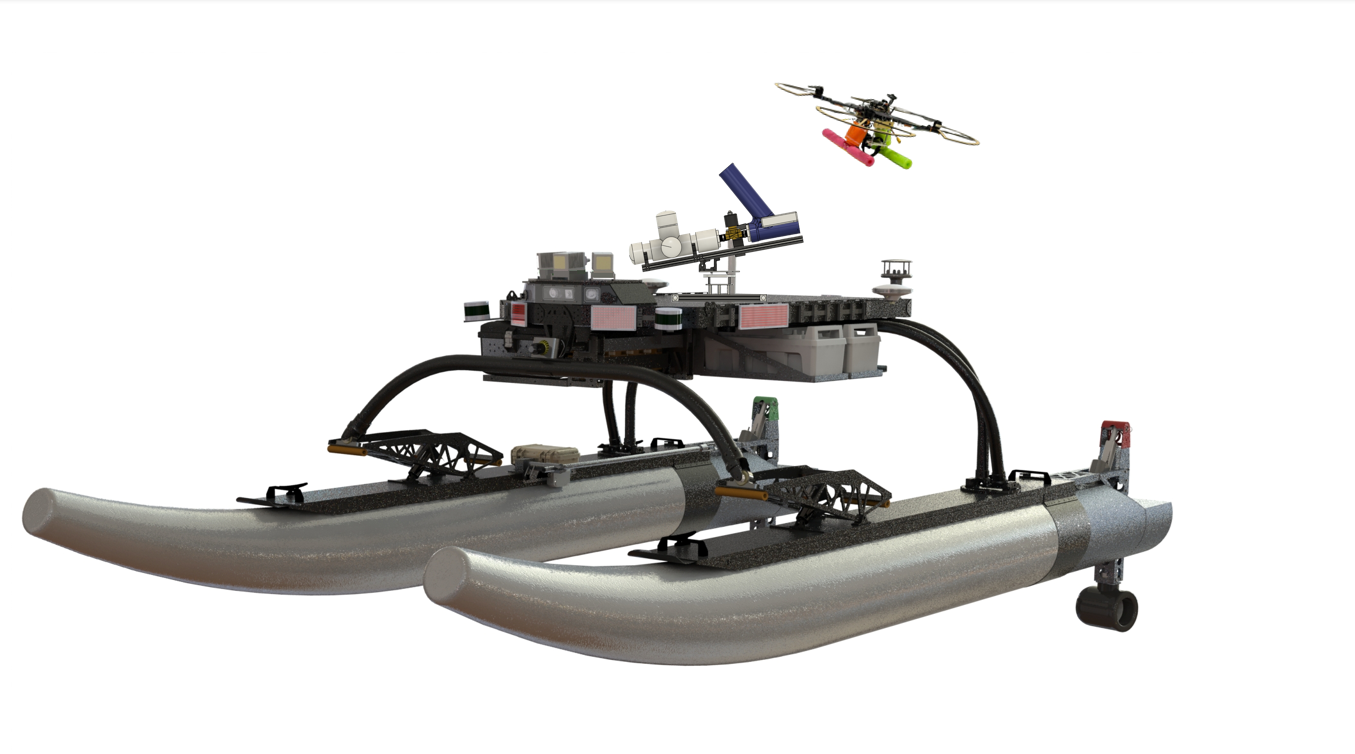
\includegraphics[width=0.8\textwidth]{Images/Minion.png}
\caption{ERAU's \ac{WAMV} Research Vessel Minion as configured for the 2024 Maritime RobotX Challenge.}
\label{fig:minion}
\end{figure}

The sensing configuration used in this research and the 2024 competition is described in Section \ref{perception_geometry}.
% The sensor configuration described in section \ref{perception_geometry} was originally developed by Team Minion for the 2022 and 2024 Maritime RobotX competitions \cite{holland2024, thompson2023}. 
Section~\ref{sensors} presents the technical specifications of Minion's sensor hardware, with particular emphasis on the \ac{LiDAR} and high-definition camera sensors selected for this study.
An overview of the CPU and network infrastructure of the system is provided in section~\ref{sec:Atlas_LAN} as background for the computational requirements of the real-time object detection methods presented in Chapter~\ref{realtime_object_detection}, as well as the challenges relating to the synchronization of sensors in section~\ref{sec:calibration}.
% housed within the forward camera enclosure. Section~\ref{visual_cameras} provides additional discussion regarding visual spectrum sensor selection and characterization. 
Of particular note, the timestamp embedding mechanism described in Section~\ref{time_sync_cam} overcomes network latency issues in the video pipeline to maintain a more precise temporal alignment.
% , essential for rigorous multi-modal sensor fusion analysis.
Finally, section~\ref{sensor_data} discusses the \ac{ROS} software architecture responsible for recording and processing sensor data.

%%%%%%%%%%%%%%%%%%%%%%%%%%%%%%%%%%%%%%%%%%%%%%%%%%%%%%%%%%%%%%%%%%%%
%%%%%%%%%%%%%%%%%%%%%%%%%%%%%%%%%%%%%%%%%%%%%%%%%%%%%%%%%%%%%%%%%%%%
\section{Perception Geometry} \label{perception_geometry}

Minion is equipped with six \ac{LiDAR} sensors as well as six cameras to perceive her surroundings.
Omnidirectional \ac{LiDAR} coverage is provided by three Velodyne VLP-16 units for situational awareness within the \acp{USV} immediate operating environment.
% \ac{LiDAR} coverage and object detection within the vessel's immediate operating environment.
Three additional forward-scanning Livox Horizon \ac{LiDAR} units generate a dense point cloud ahead of the vessel for object detection and classification at greater distances.
The Livox units are directly mounted to a camera enclosure which houses four high-definition visual-spectrum cameras and two \ac{LWIR} cameras.
The combination of forward-scanning LiDAR and cameras provides a significantly higher fidelity of data within a shared 165-degree \ac{FOV}. % in the direction of travel.
% The camera enclosure design emphasizes modularity and research flexibility.
Figure~\ref{fig:camera_enclosure} illustrates the mounting arrangement of the Livox Horizon LiDAR units and the six cameras within the waterproof enclosure.
Together, these sensors define the operational envelope of the perception system, encompassing a horizontal \ac{FOV} of approximately 160~degrees and an effective detection range of up to 60~meters.

\begin{figure}[htbp]
\centering
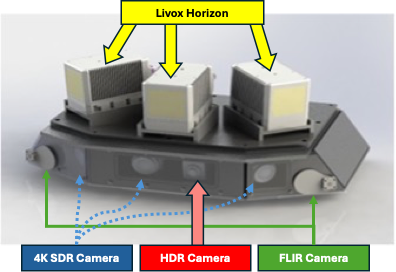
\includegraphics[width=0.6\textwidth]{Images/Camera_enclosure2.png}
\caption{Mounting locations of three Livox Horizon LiDAR units (yellow arrow, top), two LWIR cameras (green, thin, solid arrows), three FLIR 4k cameras (blue, dotted arrows), and a single \ac{HDR} camera  (red arrow, bottom) within the camera enclosure.}
\label{fig:camera_enclosure}
\end{figure}

% While the Velodyne \ac{LiDAR} sensors provide comprehensive 360-degree environmental awareness for navigation and collision avoidance, the three forward-facing Livox Horizon \ac{LiDAR} units mounted to the camera enclosure were selected for their superior point cloud density and ability to facilitate a higher resolution for object detection.
% The three Livox units concentrate sampling density in the forward \ac{FOV}, matching the horizontal coverage of the six cameras.
% Both modalities overlap the \ac{FOV} of their respective individual sensors.
% This sensor arrangement ensures higher density and more uniform point-cloud across the 165-degree forward perception envelope in the case of \ac{LiDAR}, but also makes the system more robust to failure.
% Losing a single sensor will not create a blind spot for either sensing modality in the forward path of motion of the \ac{USV}. 
% Figures~\ref{fig:fov_cam} and ~\ref{fig:fov_lidar} show how the horizontal \ac{FOV} for each of these sensors overlaps in the direction of travel.

% Each of these sensors is installed so that the center of their \ac{FOV} is parallel to one of three separate lines of vision.
% The first of these lines is a vector that points down the centerline of the vessel in the forward direction, and sensors in this orientation receive the moniker of \texttt{sensor\_center}.
% The other two lines of vision are rotated 40 degrees counterclockwise and clockwise from the centerline, and sensors in these orientations receive the moniker \texttt{sensor\_port} and \texttt{sensor\_starboard}, respectively.
Each sensor’s optical axis is aligned with one of three predefined sight lines: the vessel's centerline and two axes rotated $\pm 40$ degrees from the center.
% In the case of LiDAR, this sensor arrangement provides a denser point cloud and, in general, means that the loss of signal from any single sensor does not create a blind spot in the forward direction of travel.
For the LiDAR system, this configuration increases point-cloud density in the forward direction and ensures that loss of any single sensor does not produce a blind spot in the forward direction of travel.
% Figure~\ref{fig:fov_combined} shows the camera's \ac{FOV} in \ref{fig:fov_cam}, and the the LiDAR \ac{FOV} in \ref{fig:fov_lidar}.
Each of the three Livox Horizon LiDAR units has an 81.7-degree \ac{FOV}, resulting in more than a 40-degree overlap in the \ac{FOV} between \texttt{livox\_center} and both \texttt{livox\_port} and \texttt{livox\_starboard}, and approximately 3 degrees of overlap between \texttt{livox\_port} and \texttt{livox\_starboard} (figure~\ref{fig:fov_lidar}).
Three 4K cameras are configured to point in along each of these three sight lines. 
While these cameras are equipped with a Theia-TL410P zoom lens, they are currently set at a fixed zoom level that approximates a 65-degree horizontal \ac{FOV}, which provides a 15-degree overlap in their \ac{FOV} (figure~\ref{fig:fov_cam}).
The two \ac{LWIR} cameras each have a 90-degree \acs{FOV}, and are positioned along the port and starboard vision lines, providing a 10-degree overlap.
Finally, there is a single HDR camera with a 65-degree horizontal \ac{FOV} that points forward.
While the \ac{HDR} camera lacks any of the aforementioned sensor redundancy, its \ac{FOV} aligns with the central 4k camera and was added for research that compared the two center-line mounted cameras \cite{liebergall}.

% related to the dynamic range of the two center-line mounted cameras  and was selected as the primary visual range sensor for this body of work for reasons that are discussed in section~\ref{visual_cameras}.


\begin{figure}[htbp]
\centering
\begin{subfigure}[t]{0.48\textwidth}
    \centering
    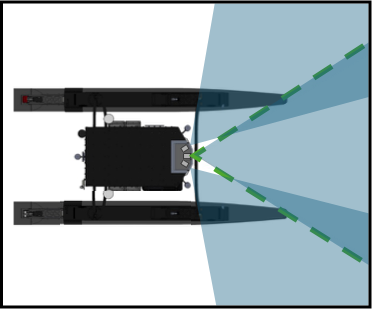
\includegraphics[width=\textwidth]{Images/fov_cam.png}
    \caption{Blue cones represent \ac{FOV} from individual FLIR 4K camera; green dashed lines indicate \ac{FOV} of HDR camera. \textcolor{red}{(This image may need to be re-created. port and sb FOV should not overlap. check fixed FOV)}}
    \label{fig:fov_cam}
\end{subfigure}
\hfill
\begin{subfigure}[t]{0.48\textwidth}
    \centering
    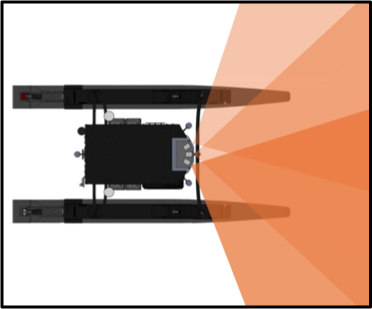
\includegraphics[width=\textwidth]{Images/fov_lidar.png}
    \caption{LiDAR horizontal \ac{FOV} overlap.}
    \label{fig:fov_lidar}
\end{subfigure}
\caption{Comparative visualization of horizontal \ac{FOV} (FOV) overlap for (a) cameras and (b) LiDAR sensors.}
\label{fig:fov_combined}
\end{figure}

% A Torc Robotics PinPoint \ac{GPS}/\ac{IMU} system is equipped with provides both global time synchronization and platform pose estimation.

% The sensor coordinate frames are organized in a hierarchical transformation tree structure, which is shown in \ref{transform_diagm}.
% The inertial reference frame (\texttt{map}) defines the world-fixed coordinate system.
% The platform reference frame (\texttt{base\_link}) represents the vessel body frame defined by the PinPoint \ac{GPS}/\ac{IMU}.
% The center Livox frame (\texttt{livox\_center}) serves as the primary sensor reference frame, with \texttt{livox\_port} and \texttt{livox\_starboard} both reporting data in the \texttt{livox\_center} reference frame.
% Six camera image frames exist within this tree, and are referenced to the \texttt{livox\_center} frame.
% Intrinsic calibration parameters, including camera-specific matrices and distortion coefficients, along with extrinsic transformation parameters relating sensor frames to each other and to the platform frame, are discussed in \textcolor{red}{Appendix \#}.

% The Livox scan pattern employs a non-repetitive rosette pattern that progressively covers the \ac{FOV} over time rather than repeatedly sampling fixed positions.
% This characteristic enables temporal aggregation to increase effective spatial resolution, particularly beneficial for a moving platform where \ac{GPS}/\ac{IMU} pose data enables motion-compensated point cloud accumulation.

% The dual \ac{LiDAR} architecture serves complementary purposes.
% The Velodyne VLP-16 units provide the omnidirectional awareness required for autonomous navigation, while the Livox Horizon sensors optimize point cloud density specifically within the forward camera \ac{FOV} for fusion research.
% The onboard This configuration enables comparative evaluation of detection performance while maintaining operational navigation capabilities.
% The sensor suite supports the research objectives of comparing detection performance across modalities and evaluating late fusion approaches.
% The following subsections detail individual sensor specifications and selection rationale.

% The primary sensors used for the data collected for this research were from the forward-facing perception module, referred to as the camera enclosure.

%%%%%%%%%%%%%%%%%%%%%%%%%%%%%%%%%%%%%%%%%%%%%%%%%%%%%%%%%%%%%%%%%%%%
%%%%%%%%%%%%%%%%%%%%%%%%%%%%%%%%%%%%%%%%%%%%%%%%%%%%%%%%%%%%%%%%%%%%
\section{Sensors} \label{sensors}

% The Minion platform integrates multiple sensor modalities to support maritime perception research.
% This section details the specifications and characteristics of the visual cameras (Section~\ref{visual_cameras}) \ac{LiDAR} systems (Section~\ref{sensors_LiDAR}), and navigation sensors (Section~\ref{gps_ins}) used in this research.
% , thermal cameras (Section~\ref{thermal_cameras}), and navigation sensors (Section~\ref{gps_ins}) 

%%%%%%%%%%%%%%%%%%%%%%%%%%%%%%%%%%%%%%%%%%%%%%%%%%%%%%%%%%%%%%%%%%%%
\subsection{LiDAR} \label{sensors_LiDAR}

% The Minion platform features six \ac{LiDAR} units providing both omnidirectional environmental awareness and forward-facing high-density perception.
% The \ac{LiDAR} suite is comprised of three Velodyne VLP-16 pucks and three Livox Horizon units.

% Three Velodyne VLP-16 \ac{LiDAR} sensors are positioned at aft-center, with the other two placed at approximately one-third intervals around the vessel at forward-port and forward-starboard, providing complete 360-degree coverage for navigation as well as object detection and avoidance.
% An additional three Livox Horizon solid-state forward-scanning \ac{LiDAR} sensors provide high-density measurements within the forward direction of motion.
Three Velodyne VLP-16 \ac{LiDAR} sensors are installed around the vessel to provide omnidirectional situational awareness. 
One unit is mounted near the aft-center position, and the other two are positioned at approximately one-third intervals around the forward-port and forward-starboard quadrants. 
Together, these sensors deliver nearly continuous 360° coverage for navigation and obstacle avoidance.

Each VLP-16 employs 16 lasers arranged in a vertical array that scans 16 distinct points elevation over its 30-degree vertical \ac{FOV} continuously over the 360-degree azimuth, producing approximately 300,000 \ac{pps} in single-return mode. 
The units are installed with a downward declination of approximately 5 degrees from the plane of the \ac{USV} deck to minimize blind-spots near the vessel's waterline.
As a result, one-half to one-third of their scanning azimuth is well above the horizon or pointing directly into the vessel and is discarded, drastically reducing the number of points each unit can publish.

% Both of these units are capable of approximately 1.4 million measurements per second.
% For an equivalent 80-degree horizontal FOV, the Velodyne’s effective $317,700 \text{ pts/sec}$ represents $\approx 22 \%$ of the overlapping \ac{FOV} of the Livox unit’s output.
% % While each Velodyne VLP-16 unit is capable of producing 300k \ac{pps} compared to the Livox unit's 280k, their 360-degree scanning pattern means that only 
% The principal distinction between them lies in their underlying scanning architectures and sampling density, which directly influences perception fidelity.
% The Velodyne VLP-16 LiDAR scans 16 discrete points spanning a 30-degree vertical \ac{FOV} emanating from the azimuthal plane of the device in a 360-degree horizontal \ac{FOV}that repeats identically with each rotation. 
% The points generated span the 360
% % To minimize blind spots near the base of Minion, each of the Velodyne units is mounted at a 15-degree declination from the vessel's deck plane, resulting in 
% These rings are notF
% % For vessels moving at typical speeds (2-5 m/s), platform displacement between rotations remains small relative to object size, resulting in near-perfect overlap of consecutive scans.
% At typical vessel speeds between $2 \text{to} 5 m/s$, successive Velodyne rotations overlap almost perfectly, causing sparse sampling of small or distant targets.
% % This means that small to medium-sized objects may not even be detected when at large distances from the sensor, as illustrated in Figure \ref{fig:lidar_scan_compare}.
% Consequently, small or distant targets may be undersampled or entirely missed in sequential Velodyne frames (Figure \ref{fig:lidar_scan_compare}).

In contrast, the three Livox Horizon solid-state \ac{LiDAR} units concentrate their scanning pattern within an $81.7 \times 25.1$ degree \ac{FOV}, generating up to 280,000 \ac{pps}. 
Although the nominal point rates are comparable, the Livox pattern can return $100 \%$ of its concentrated \ac{FOV} data. 
This higher spatial sampling density enables detection and classification of objects that may be smaller or further from the sensor.
A direct comparison of the discrepancy between the Velodyne and Livox scan patterns and point density is provided in Figure \ref{fig:lidar_scan_compare}.
The top-right image shows the dense point cloud of the Livox devices.
The light tower in the foreground and the large dock structure in the background can be seen in the camera view (left) and are both well defined in the red point cloud.
Two small buoys are also distinctly visible between the two structures.
In comparison, the point cloud returned by the Velodyne devices is shown in the bottom-right. 
The general form of the light tower can be seen; however, there are very few points returned from the large dock structure in the background, and the round buoys are undetected.

% The forward-scanning Livox devices operate differently, tracing a non-repetitive pattern across the \ac{FOV}.
% Two orthogonal mirrors oscillate at slightly different frequencies to cause the laser beam to trace a path that progressively fills the \ac{FOV} without repetition as shown in Figure ~\ref{fig:livox_scan_pattern}.

\begin{figure}[htbp]
\centering
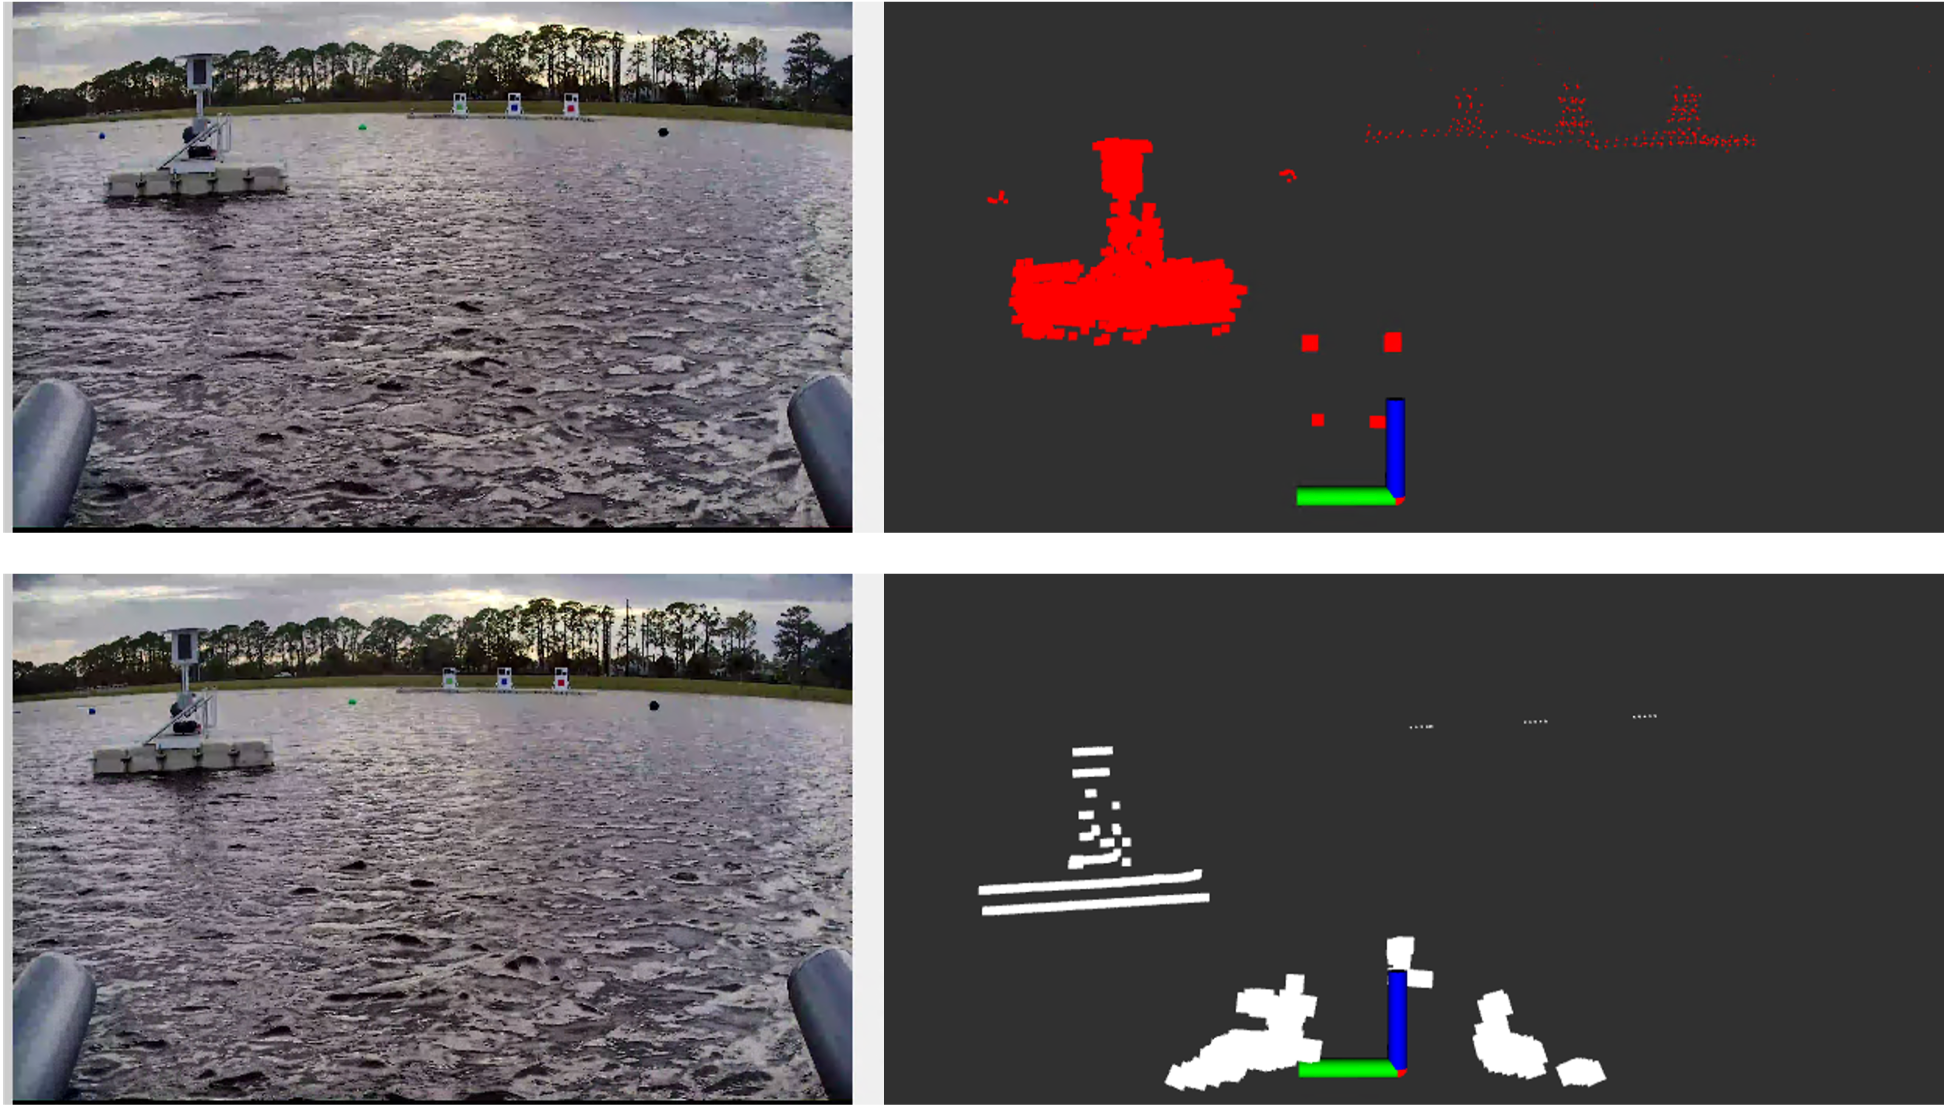
\includegraphics[width=0.8\textwidth]{Images/LiDAR_compare.png}
\caption{A comparison of LiDAR returns from the Livox units (top-right, red) and Velodyne units (bottom-right, white) to the respective HDR camera view (top-left and bottom-left). LiDAR points are viewed from third-person point of view in RVIZ. Green and Blue axes (top-right, top-bottom) represent the origin of the USV frame of reference.}
\label{fig:lidar_scan_compare}
\end{figure}

% The superior point density of the overlapping forward-scanning  LiDAR is critical for the real-time object detection method that is discussed in \textcolor{red}{Section \#}.
% The overlapping forward-scanning LiDAR provides the spatial density required for the real-time object-detection framework described in Section \ref{gbcache}.
% For this reason, the research presented in this work exclusively utilizes LiDAR data from the Livox Horizon sensors.

Consequently, the research presented in this work relies exclusively on LiDAR data from the forward-scanning Livox Horizon sensors, whose concentrated and non-repetitive coverage provides the spatial resolution required for the real-time object-detection framework described in Section \ref{gbcache}.
        %%%%%%%%%%%%%%%%%%%%%%%%%%%%%%%%%%%%%%%%%%%%%%%%%%%%%%%%%%%%
\subsubsection{Livox Horizon} \label{sensors_livox}

% Each Livox Horizon employs two orthogonal mirrors operating at different frequencies to trace a complex Lissajous-like path that progressively fills the $81.7 \times 25.1$-degree (horizontal × vertical) \ac{FOV}, as illustrated in Figure~\ref{fig:livox_scan_pattern}. 
% The three Livox units are mounted with 40 degrees of horizontal separation, overlapping each other \ac{FOV} by $\approx 50\%$, making the system robust to failure of any single unit, as well as effectively doubling the rate of sampled points and distributing them more evenly across the center device's \ac{FOV}. 
Each Livox Horizon uses dual orthogonal mirrors oscillating at slightly different frequencies to generate a non-repetitive Lissajous-like scan pattern over its $81.7 \times 25.1$ degree \ac{FOV}. 
Overlapping these sensors by roughly $50 \%$ effectively doubles the point density along the center-line path under nominal operation, and maintains coverage under single-unit failure.
Table~\ref{table:livox_horizon_specs} presents detailed hardware specifications for the Livox Horizon.

% The rosette scan pattern is provided in \ref{fig:livox_scan_pattern}, and table \ref{table:livox_horizon_specs} presents the Livox Horizon specifications.


 
\begin{figure}[htbp]
\centering
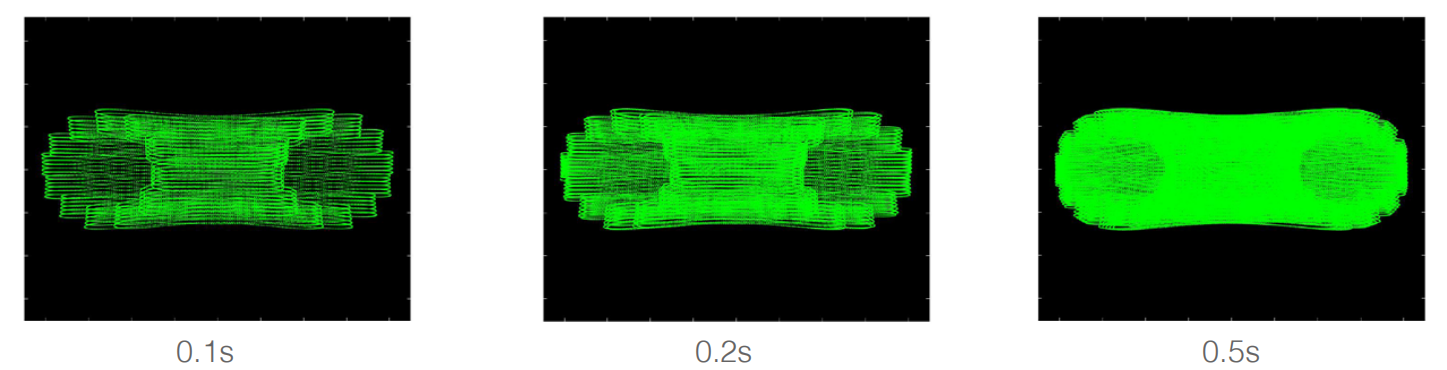
\includegraphics[width=0.8\textwidth]{Images/Livox_1.png}
\caption{Livox Horizon non-repetitive rosette scan pattern demonstrating point cloud density distribution from 0.1 to 0.5 seconds. Provided by \cite{livox_manual}}
\label{fig:livox_scan_pattern}
\end{figure}


Each device is capable of returning up to $4.8 \times 10^5$ \ac{pps} in dual return mode, with each return consisting of position coordinates (x, y, z), target reflectivity, and timestamp.
This operational mode returns two data points for each laser emission and is useful for situations where the sensor scans semi-permeable objects such as windows, thick tree canopies, or water.
% Instead, each device is operated in single-return mode for two reasons.
% The first is a consideration of available network bandwidth.
Each sensor operates in single-return mode, primarily to reduce network load.
A conservative estimate of 16 bytes per point results in $\approx 23 \text{ Mbps}$ which would quickly overwhelm the \ac{USV}'s network.
% Luckily, the 905 nm near-infrared wavelength of the emitted laser experiences strong absorption by water. 
However, The $905 nm$ near-infrared emission is strongly absorbed by water, effectively suppressing subsurface returns.
This means that only points which are reflected by the water surface are returned with an intensity greater than zero, making it straight forward to filter out points in the ground plane.

\begin{table}[htpb]
\centering
\begin{tabular}{ll}
\hline
\multicolumn{2}{c}{Livox Horizon}\\
\hline
% \textbf{Parameter} & \textbf{Value} \\
\hline
Model & Livox Horizon \\
Horizontal Field of View & 81.7 degree \\
Vertical Field of View & 25.1 degree \\
Range & 260 m @ 80\% reflectivity \\
Point Rate (Single Return) & 240,000 pts/sec \\
Point Rate (Dual Return) & 480,000 pts/sec \\
Range Precision & ±2 cm \\
Wavelength & 905 nm \\
Scan Pattern & Non-repetitive rosette \\
Interface & Ethernet \\
Operating Frequency & 100 Hz \\
\hline
\end{tabular}
\caption{LiDAR Specifications}
\label{table:livox_horizon_specs}
\end{table}


%%%%%%% move to sensor calibration %%%%%%%%%%%
% Accurate fusion of data from multiple \ac{LiDAR} units requires precise knowledge of sensor geometric relationships.
% The Livox Horizon units feature onboard storage for extrinsic calibration parameters, enabling each sensor to transform its measurements to a common reference frame before transmission.
% These parameters are written to non-volatile memory on each Livox unit and applied before data transmission so that all LiDAR returns are received in the center \ac{LiDAR}'s reference frame, reducing the necessary calculation further down the data pipeline.
% \textcolor{red}{cite Livox documentation?}.
% enhancing their real-time operational advantage by reducing additional computation later in the pipeline.
% The calibration methodology to determine these extrinsic values is detailed in Section~\ref{lidar_extrinsic}.
%%%%%%%%%%%%%%%%%%%%%%%%%%%%%%%%%%%%%%%%%%%%%%%

% The 905 nm near-infrared wavelength experiences strong absorption by water, resulting in minimal returns from water surfaces.
% This characteristic benefits maritime object detection by reducing clutter from waves that would otherwise trigger false positives in clustering algorithms.

% The fundamental distinction between the Livox Horizon and traditional spinning \ac{LiDAR} lies in the scan pattern.
% A mechanically spinning sensor with N lasers produces N discrete horizontal rings that repeat identically each rotation.
% For vessels moving at typical speeds (2-5 m/s), platform displacement between rotations remains small relative to object size, resulting in near-perfect overlap of consecutive scans.
% The Livox operates differently, employing a two-dimensional scanning mechanism that traces a non-repetitive rosette pattern across the \ac{FOV}.
% Two orthogonal mirrors operating at slightly different frequencies cause the laser beam to trace a complex Lissajous-like path that progressively fills the \ac{FOV} without repetition \cite{thompson2023}.

% Scan pattern coverage accumulates over time, with longer integration periods yielding denser spatial sampling.
% At the standard 100 Hz output rate, each \ac{UDP} message contains approximately 10 milliseconds of returns.
% Over a one-second aggregation period, the rosette pattern provides substantially higher spatial coverage than a spinning sensor's fixed ring geometry.

% The non-repetitive forward-scanning nature of the Livox units means that point cloud density is not uniform across the \ac{FOV}.
% The 81.7-degree horizontal \ac{FOV} allows for overlap between the three units, achieving more uniform density across the 165-degree \ac{FOV}, matching the 4K FLIR camera coverage.

% Insert figure showing Livox scan pattern here
% \begin{figure}[htbp]
% \centering
% 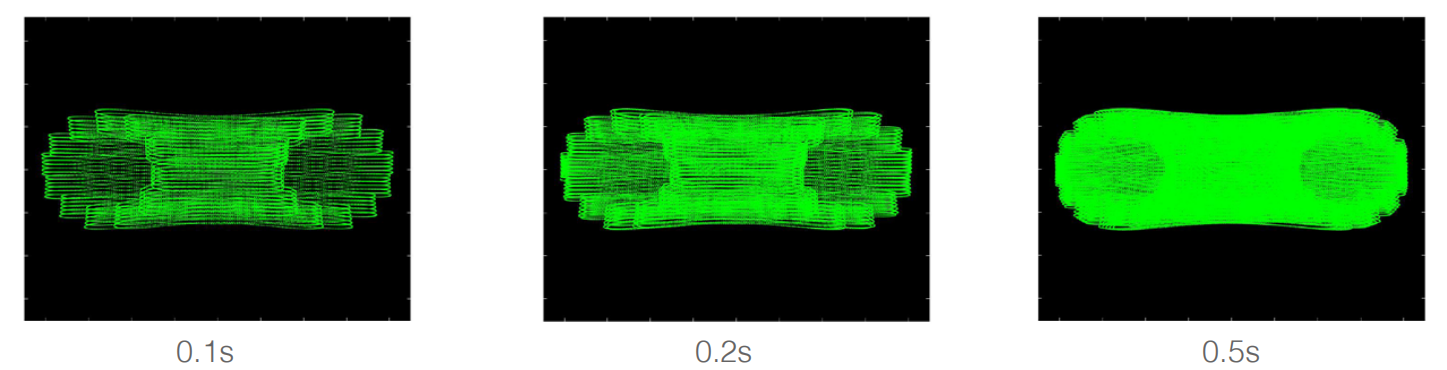
\includegraphics[width=0.8\textwidth]{Images/Livox_1.png}
% \caption{Livox Horizon non-repetitive rosette scan pattern demonstrating point cloud density distribution from 0.1 to 0.5 seconds.}
% \label{fig:livox_scan_pattern}
% \end{figure}




% A Velodyne VLP-16 in dual-return mode produces approximately 1.4 million \ac{pps} distributed across the full 360-degree plane.
% The camera \ac{FOV} encompasses approximately 165 degrees, yielding an effective point rate in the region of interest of:

% $$\text{Effective HDL-32E rate} = 1.4 \times 10^6 \times \frac{165 degree}{360 degree} \approx 641,000 \text{ pts/sec}$$

% Three Livox Horizon units in dual-return mode together produce:

% $$\text{Combined Livox rate} = 3 \times 480,000 = 1.44 \times 10^6 \text{ pts/sec}$$

% This represents a 2.25× increase in point returns within the camera view, excluding additional benefits from superior vertical sampling achieved through the non-repetitive pattern compared to fixed 32-ring geometry \cite{thompson2023}.

%%%%%%%%%%%%%%%%%%%%%%%%%%%%%%%%%%%%%%%%%%%%%%%%%%%%%%%%%%%%%%%%%%%%
\subsection{Visible Spectrum Cameras} \label{visual_cameras}

% \textcolor{red}{Expand this entire discussion}
% The visible spectrum camera suite on the Minion platform is designed to balance two factors that are particularly important for maritime perception: imaging resolution and dynamic range.

For computer vision and perception tasks, system performance is directly influenced by the quality of the visual input.
The fidelity of an image is determined by a camera's hardware and integrated software; therefore, camera selection is a critical design consideration in any vision-based system. 
Sensor size and lens characteristics determine the spatial detail captured, while shutter speed, exposure, and onboard processing influence brightness, contrast, and color balance. 
The visible-spectrum cameras housed within the camera enclosure were selected to balance image resolution and dynamic range, two essential factors for reliable maritime perception.
A brief discussion of both of these metrics is presented here to justify utilizing data acquired from the \ac{HDR} camera for this research.

\subsubsection{Image Resolution}
Camera resolution determines the ability to resolve small targets at a distance.
% , and appropriate imaging sensors and lenses can be selected by determining the maximum distance and minimum size at which objects need to be resolved.
% Camera resolution dictates the minimum discernible target size at range; lens and sensor parameters are therefore chosen to meet specified detection distances.
% Camera resolution governs the minimum resolvable target size; lens and sensor parameters are thus selected to ensure detection at required ranges.
To ensure adequate perception across the operational envelope, cameras must resolve objects to a required minimum resolution when the object is at the maximum detection range.
% The resolution of an object in the image frame can be determined if the object's width $\mathit{l}$ and distance from the camera $d$ are knownwith
The relationship between an object's physical width $\mathit{w}_{obj}$ and pixel width within an image $\mathit{w}_{\text{px}}$ is given by
% Provided a maximum detection range $d$ and the width of the smallest object to be detected $W$, the camera's focal length and resolution requirements can be determined by assuming a pinhole-camera model \cite{matlab_calibration}, can be derived as:
% we can determine the necessary optical focal length and resolution for the sensor.
% For an object of physical width $W$ at distance $d$, its width in the image frame $w_{\text{px}}$ is approximated by

\begin{equation}
\mathit{w}_{\text{px}} = f \; \frac{N_x}{S_w}\frac{\mathit{w}_{obj}}{d}
\end{equation}

% where $\mathit{l}_{\text{px}}$ is the pixel width of an object in the image frame, 
where $f$ is the \ac{EFL} of the camera and lens, $N_x$ is the horizontal image resolution in pixels, and $S_w$ is the width of the image sensor.
% This equation is used for sensor selection by determining the minimum resolution required for the smallest object to be detected at the maximum detection range.
This equation can be used to determine camera requirements if the true size of the imaged objects is known, or to determine a reasonable expectation of object resolution if the camera values are known.
This relationship is also critical for determining the distortion present in each camera/lens system, detailed further in section~\ref{HDR_intrinsic}.

Defining the requirement for the minimum resolution of an object in the image frame requires an understanding of the object detection method used with visual cameras, as well as the objects being detected. both of which will be discussed in greater detail in sections ~\ref{dataset} and ~\ref{yolo}, respectively.
% For now, it is sufficient to know that the smallest object we wish to detect is $0.3683$ meters wide at a distance of 60 meters.
% , and that we have optical and digital resolution requirements to consider.
This image detection architecture is discussed in section ~\ref{yolo}.
For camera selection, it is sufficient to know that this method scales down each input image to a resolution of $640 \times 640$ pixels for processing efficiency.
This should be considered when defining the minimum pixel density of a camera's sensor, as it alters our prior equation slightly.

\begin{equation}
\mathit{w}'_{\text{px}} = f \; \frac{640 \text{px}}{S_w}\frac{\mathit{w}_{obj}}{d}
\end{equation}
% This means that an image captured at $4000 \times 3000$ pixels is reduced to $650 \times 487$ pixels, which is $16.25\%$ of its original size.
% As an example, if the text on waterway signage 60 meters away is legible at a resolution of 100 pixels wide in a 1,000 $\times$ 1,000 pixel image, it would need a resolution of 162 pixels to meet the additional requirements imposed by the image detection algorithm.
Each camera within the enclosure was selected using these metrics, and object information based on the obstacles commonly associated with the RobotX Maritime Challenge. %, in addition to other contemporaneous research \cite{thompson2023} \textcolor{red}{(check scholarly commons)}.

% \textcolor{red}{add back: ?}
Given that the smallest object we wish to detect is $0.3683$ meters wide at a distance of 60 meters.
The two visual spectrum camera models within the camera enclosure have a similar focal length, and resolutions of $4000 \times 3000$ px and $2880 \times 1860$ px. Examining the camera with the smaller horizontal resolution of 1880 px (which has a sensor width of $S_{w} = 8.64$ mm), we obtain the width of our object in the image frame as
% meet this requirement; the object detection method used will impose a secondary constraint.
\begin{equation*}
\begin{split}
    \mathit{w}_{\text{px}} & = 8\;\text{mm} \cdot \frac{2880\;\text{px}}{8.64\;\text{mm}} \cdot \frac{0.3683\;\text{m}}{60\;\text{m}}\\
     & = 16.36 \approx 16 \;\text{px}
\end{split}
\end{equation*}

With the additional scaling required by the visual object detection method, the minimum width of our object becomes 
\begin{equation*}
\begin{split}
    \mathit{w}'_{\text{px}} & = 16\;\text{px} \cdot \frac{640\;\text{px}}{2880\;\text{px}} \\
     & = 3.\overline{55} \approx 3 \;\text{px}
\end{split}
\end{equation*}

Figure \ref{fig:A2_multi_res} shows our smallest object, Polyform A2 round buoy, at a selection of resolutions, and is still recognizable at a resolution of 16 pixels wide. %, and becomes less defined at lower resolutions. 
This operation is repeated to predict the width of the object in the image frame at a range of distances up to our maximum of 60 meters, and the results are provided in Table \ref{table:buoy_res}.
From this information, the buoy will be easily recognizable at any range by visual inspection, but will become much less defined when the image is scaled down for the visual object detection method.
As we will discuss in section \ref{yolo}, this method may struggle to detect this size buoy at distances greater than 20 meters.

\begin{table}[htpb]
\centering
\begin{tabular}{c|c|c}
\hline
\multicolumn{3}{c}{Polyform A2 Buoy Resolution at Range}\\
\hline
% \textbf{Parameter} & \textbf{Value} \\
\hline
Object Distance & Image Frame Width & With Detection \\
\hline
10 m & 98 px & 21 px \\
20 m & 49 px & 10 px \\
30 m & 32 px & 7 px \\
40 m & 24 px & 5 px \\
50 m & 19 px & 4 px \\
60 m & 16 px & 3 px \\
\hline
\end{tabular}
\caption{The predicted resolution of a $\mathit{l} = 0.3683$ meter wide object within the Loepard Imaging HDR camera's image frame at multiple distances.}
\label{table:buoy_res}
\end{table}

\begin{figure}[htbp]
\centering
\begin{subfigure}[t]{0.245\textwidth}
    \centering
    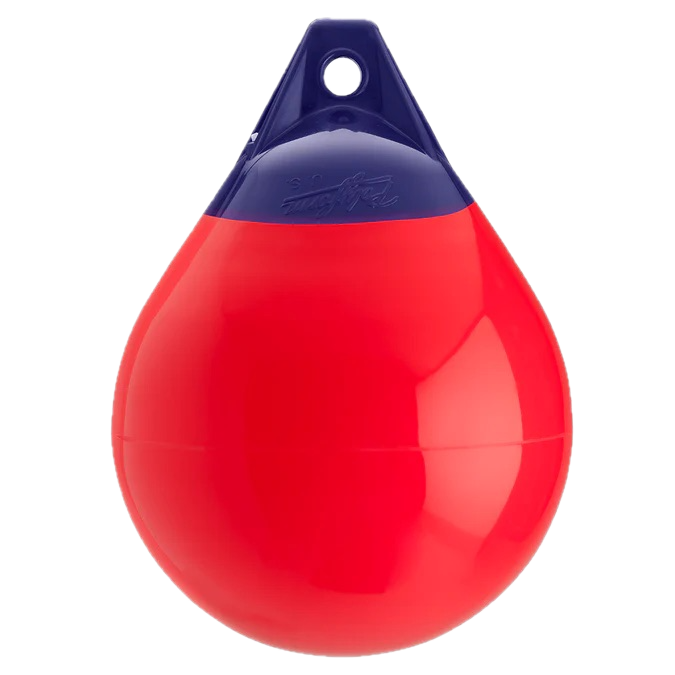
\includegraphics[width=\textwidth]{Images/A2.png}
    \caption{\raggedright{Polyform A2 Buoy}}
    \label{fig:A2}
\end{subfigure}
\hfill
\begin{subfigure}[t]{0.245\textwidth}
    \centering
    
\includegraphics[width=\textwidth]{Images/A2_16px.png}
    \caption{
    16 pixel width,\\  
    % $\approx$ 60 m with HDR
    }
    \label{fig:A2_16px}
\end{subfigure}
\hfill
\begin{subfigure}[t]{0.245\textwidth}
    \centering
    
\includegraphics[width=\textwidth]{Images/A2_6px.png}
    \caption{
    6 pixel width,\\  
    % $\approx$ 40 m with HDR \\ 
    % \& object detection.
    }
    \label{fig:A2_6px}
\end{subfigure}
\hfill
\begin{subfigure}[t]{0.245\textwidth}
    \centering
    
\includegraphics[width=\textwidth]{Images/A2_3px.png}
    \caption{
    3 pixel width,\\  
    % $\approx$ 60 m with HDR \\ 
    % \& object detection.
    }
    \label{fig:A2_3px}
\end{subfigure}
\caption{Polyform A2 Buoy (a), visualized at 16 pixels (b), 6 pixels (c), and 3 pixels wide (d).}
\label{fig:A2_multi_res}
\end{figure}


% Insert equation to get the horizontal focal length / horizontal resolution ratio needed for camera selection based upon the equation and information provided above
% Assuming our camera will have a landscape aspect ratio, our equation becomes 
% Since the detection network downsamples each input frame to a maximum dimension of 640 pixels while preserving aspect ratio, a landscape-oriented image with native resolution $N_x \times N_y$ (where $N_x > N_y$) is scaled such that the horizontal dimension becomes 640 pixels.
% For an object that must occupy at least $w_{\text{net}}$ pixels horizontally in the network input to be reliably detected, the camera system must satisfy
%   \begin{equation}
%   \frac{f}{S_w} = \frac{w_{\text{net}} \, d}{640 \, W}
%   \end{equation}
% \begin{equation}
%  w_{\text{px}} \left(\frac{650}{N_x}\right) = f \; \frac{N_x}{S_w}\frac{W}{d}
% \end{equation}

% where the ratio $f/S_w$ represents the normalized focal length of the camera-lens system.
% Substituting the minimum object dimensions ($W = 0.3683$ m, $d = 60$ m) and assuming a minimum network resolution requirement of $w_{\text{net}}$ pixels, this relationship defines the optical design space for camera selection.
% This makes our equation

% \begin{equation}
% w_{\text{px}} = \frac{f \, N_x^2 \, W}{(680)S_w \, d}
% \end{equation}



% The dynamic range of an imaging sensor refers to the range of signal intensities it can detect, and can be as critical as image resolution when selecting camera sensors.
\subsubsection{Dynamic Range}
Dynamic range describes the ratio between the brightest and darkest signal levels a camera sensor can record.
Light levels that exceed the camera sensor's range cause the image to appear white or "blown-out", while light levels that are too low will appear darker, with detail being indistinguishable from noise.
% Dynamic range—the span of detectable signal intensities—is equally critical to sensor selection as spatial resolution.
\acp{USV} and \acp{AGS} routinely operate in environments where bright sky reflections and deep shadows are common, often within the same scene.
Therefore, selecting a camera with insufficient dynamic range may lead to washed-out highlights or lost detail in shadows.

Dynamic range, expressed in dB, is given by
\begin{equation}
 \text{Dynamic Range (dB)} = 20 \log{\left( \frac{N_{sat}}{N_{noise}}\right) }
\end{equation}
where $N_{sat}/N_{noise}$ is the ratio of the saturation to the minimum signal a camera sensor can detect above background noise.
% Higher dynamic range can be achieved through software by combining sequential multi-exposure images, or through a digital overlap \ac{HDR} (DOL-HDR) architecture with in-pixel dual conversion gain.
% Sequential multi-exposure \ac{HDR}, which stacks separate frames and is prone to ghosting or blurring, therefore 
% DOL-\ac{HDR} is preferred when precise synchronization of the imagery is required, such as sensor fusion.
% Because maritime environments routinely present both bright sky reflections and deep shadows in the same scene, dynamic range is as critical as resolution when selecting cameras for perception tasks. 
High-dynamic-range (HDR) imaging can be achieved in two primary ways. 
The first is sequential multi-exposure \ac{HDR}, in which multiple frames captured at different exposure settings are combined to extend the tonal range \cite{Reinhard2010}. An example is provided in Figure \ref{fig:hdr_example}.



While effective for static scenes, this approach introduces motion-related artifacts such as ghosting and motion-blur as the relative velocity increases between the sensor and objects within the frame.
The second method uses an in-sensor technique called dual-conversion gain (DCG) that combines multiple light exposure levels within a single frame of exposure. 
% \textcolor{red}{Coyle: It isn't short and long exposure, but changing the size of the exposure pixel to capture more/less light from my understanding. This is why it doesn't motion blur} By capturing short and long exposure data within a single frame, this method avoids the distortion of multi-exposure \ac{HDR}.
The two visible sensing technologies considered for this research are described below.

\begin{figure}[htbp]
    \centering
    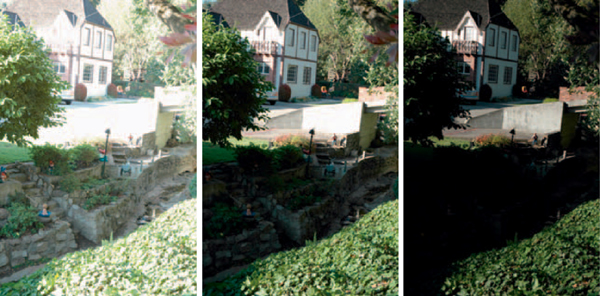
\includegraphics[width=0.65\linewidth]{Images/hdr_example.png}
    \caption{An example of multi-exposure HDR frame-stacking \cite{Reinhard2010}.}
    \label{fig:hdr_example}
\end{figure}
%%%%%%%%%%%%%%%%%%%%%%%%%%%%%%%%%%%%%%%%%%%%%%%%%%%%%%%%%%%%%%%%%%%%
\subsubsection{FLIR Blackfly S 4K Cameras} \label{sensors_FLIR}

% Three FLIR Blackfly S 4K visible-light cameras, arranged to provide a combined 165 degrees of forward-facing coverage through overlapping 65-degree lenses.  
Three FLIR Blackfly S 4K cameras are aligned to the port, center, and starboard sight-lines described in section \ref{perception_geometry} to provide a combined 165-degree horizontal \ac{FOV}.
In addition to redundancy, this configuration avoids additional spherical distortion within the image that would be required to cover the same \ac{FOV} with fewer cameras.
% Each camera is paired with a Theia TL410P zoom lens with an \ac{EFL} of \textcolor{red}{???} and an image resolution of $4096 \times 4096$, ensuring that objects remain adequately resolved across the vessel's perception envelope.  
Each FLIR Blackfly has a resolution of 4096 $\times$ 4096 pixel resolution and is paired with a Theia TL410P zoom lens at a fixed \ac{EFL} $\approx$ 8 mm.
% This sensor dimension and \ac{EFL} exceeds the pixel density required to ensure object resolution across the operational envelope.


\begin{table}[htbp]
\centering
\begin{tabular}{ll}
\hline
\multicolumn{2}{c}{FLIR 4K SDR Camera}\\
% HDR & Camera\\
\hline
% \textbf{Parameter} & \textbf{Value} \\
\hline
\multicolumn{2}{c}{Camera Sensor}\\
\hline
FLIR & Blackfly S 120S4C \\
% Image Sensor & Sony IMX490 \\
% Pixel Size & $3.0 \times 3.0 \mu m$ \\
Horizontal Resolution & 4000 pixels \\
Vertical Resolution & 3000 pixels \\
Aspect Ratio & 1.33:1 \\
Maximum Frame Rate & 31 fps \\
Dynamic Range & 69.4 dB \\
\multicolumn{2}{c}{Camera Lens}\\
\hline
Theia & TL410P\\
% Aperture F/\# & $2.0$ \\
Horizontal \Ac{FOV} & 65-degrees\\
Lens \Ac{EFL} & approx. 8 mm\\
% Vertical Field of View & 37 degrees \\
\hline
\end{tabular}
\caption{FLIR 4K SDR Camera Specifications}
\label{table:SDR_camera_specs}
\end{table}

The Blackfly S sensor captures video at 31 \ac{fps} and achieves a dynamic range of 69.4 dB, which is within the \ac{SDR}.
% This corresponds to a span of a few thousand-to-one between the darkest detectable signal and the brightest non-saturating signal.  
% The cameras capture 31 \ac{FPS} at a resolution of 4096 $\times$ 2160 pixels.
% \textcolor{red}{Add discussion of pixel density sensor selection in the context of the requirement to resolve specific objects at a minimum resolution at a maximum specific distance. This will require equations.}

%%%%%%%%%%%%%%%%%%%%%%%%%%%%%%%%%%%%%%%%%%%%%%%%%%%%%%%%%%%%%%%%%%%%
\subsubsection{Leopard Imaging HDR Camera} \label{sensors_HDR}

% A Leopard Imaging LI-USB30-IMX490-GW5400-GMSL2-065H camera, based on Sony’s IMX490 automotive-grade \ac{HDR} sensor, provides 65-degree of forward \ac{FOV}.  
The Leopard Imaging camera provides a 65-degree forward \ac{FOV} using Sony’s automotive-grade IMX490 sensor with 120 dB of dynamic range.
The \ac{HDR} is achieved via Sony’s \ac{DOL-HDR} architecture, which combines large and small photodiodes within each pixel on the sensor.
Each size of sub-pixels experience a different photon flux during each frame of exposure, and each output is read at both high and low conversion gains.
This method yields 4 measurements of light intensity within each captured frame, eliminating motion artifacts and enabling precise temporal alignment for sensor fusion.
Table \ref{table:hdr_camera_specs} provides detailed specifications for the HDR camera, which delivers a resolution of $2880 \times 1860$ pixels at 25 frames per second with a dynamic range of 120~dB
% Sony’s \ac{DOL-HDR} architecture exposes both sub-pixels (SP1 and SP2) simultaneously but reads them sequentially at different conversion gains to capture multiple brightness levels within a single frame.
% It utilizes two sizes of sensing pixels, one large and one small, which receive different flux of of photons per exposure,  within a single frame period. \textcolor{red}{Coyle: use same terminology as where you described this earlier.}
.%, extending the span of detectable light intensity to nearly one million-to-one.  

% The IMX490 accomplishes this \ac{HDR} using a digital overlap \ac{HDR} (DOL-HDR) architecture with in-pixel dual conversion gain.  

% This method captures multiple effective exposures within a single frame period, producing simultaneous multi-gain readouts from the same scene.  
% This architecture produces simultaneous multi-gain readouts without sequential stacking, 

\begin{table}[htpb]
\centering
\begin{tabular}{ll}
\hline
\multicolumn{2}{c}{Leopard Imaging HDR Camera}\\
% HDR & Camera\\
\hline
% \textbf{Parameter} & \textbf{Value} \\
\hline
% Make & Leopard Imaging \\
Leopard Imaging & LI-IMX490-GW5400-GMSL2-065H \\
Image Sensor & Sony IMX490 \\
Pixel Size & 3.0 $\times$ 3.0 $\mu$m \\
Horizontal Resolution & 2880 pixels \\
Vertical Resolution & 1860 pixels \\
Aspect Ratio & 1.55:1 \\
Maximum Frame Rate & 25 fps \\
Dynamic Range & 120 dB \\
Aperture F/\# & $2.0$ \\
Horizontal \Ac{FOV} & 65-degrees \\ %(H), 37-degrees (V) \\
% Vertical Field of View & 37 degrees \\
Lens \Ac{EFL} & 7.9 mm\\
\hline
\end{tabular}
\caption{Leopard Imaging HDR Camera Specifications}
\label{table:hdr_camera_specs}
\end{table}


% This performance is enabled by a digital overlap \ac{HDR} (DOL-HDR) architecture with in-pixel dual conversion gain.  
% By capturing multiple gain levels within a single frame period, the sensor produces simultaneous multi-gain readouts without relying on sequential multi-exposure stacking.  
% This design eliminates ghosting and motion artifacts, which are common when either the platform or surrounding targets move between exposures.  

% \subsubsection{Leopard Imaging HDR Camera}

% To overcome these limitations, a \ac{HDR} camera from Leopard Imaging was integrated, based on Sony’s IMX490 automotive-grade \ac{HDR} sensor.  
% This camera provides 65 degrees of forward coverage and achieves approximately 120~dB of dynamic range, enabling preservation of fine image details across extreme lighting conditions, including bright sky, reflective water, and shaded objects.  



% This substantial increase in dynamic range, combined with robust performance under challenging illumination, made the IMX490-based \ac{HDR} camera the primary visual spectrum sensor for \ac{LiDAR}-camera fusion research in this dissertation.  
% Preliminary results from a comparative study by Liebergall et al.~\cite{liebergall} further supported this decision, showing improved detection consistency with the \ac{HDR} sensor compared to the FLIR 4K cameras.  
% Although later published results did not fully corroborate the preliminary findings, those results became available only after the dataset for this research had been collected.  
% Accordingly, the IMX490 \ac{HDR} camera served as the main forward-facing visual spectrum sensor throughout this study.  



% The 2880×1860 resolution provides sufficient spatial detail for detecting objects at relevant ranges in autonomous vessel navigation, while the 25 fps frame rate adequately supports typical vessel speeds and maneuvering.

% The IMX490's native \ac{HDR} combines multiple exposures in a single frame period, achieving 120 dB dynamic range without sequential multi-exposure capture.
% This simultaneous approach eliminates motion artifacts associated with temporal bracketing, which is critical when both the platform and targets are in motion.
% Image quality validation and intrinsic calibration are addressed in Section 3.2.1.1, including lens distortion characterization and camera matrix estimation.
% The combination of wide dynamic range, moderate resolution, and calibrated geometry provides the image quality necessary for training and evaluating vision-based detection models in Chapter 5.

% Thompson et al. \cite{thompson2023} originally developed this camera hardware and integration approach, establishing a foundation for maritime perception research.
% The primary enhancement introduced in this work comprises in-band timestamp embedding and temporal drift correction, detailed in Section 3.2.2, which are essential for rigorous multi-modal sensor fusion analysis.

%%%%%%%%%%%%%%%%%%%%%%%%%%%%%%%%%%%%%%%%%%%%%%%%%%%%%%%%%%%%%%%%%%%%
\subsubsection{Camera Selection} \label{camera_selection}

The combination of image resolution and \ac{EFL} of both cameras exceeds the pixel density required to ensure object resolution across the operational envelope.
\textcolor{red}{Coyle: which you never told me}
FLIR Blackfly S 4K cameras exceed the resolution requirements, but their limited dynamic range of 69.4~dB makes them prone to over-exposure and reduced contrast under extreme lighting conditions. 
% They support an effective dynamic range of 69.4~dB, which corresponds to a span of just a few thousand-to-one between the darkest detectable signal and the brightest non-saturating signal. 
% As a result, the cameras are prone to over-exposure in high-brightness maritime conditions, particularly when imaging reflective water surfaces or bright sky backgrounds, leading to loss of highlight detail and reduced contrast. 

\begin{figure}[htbp]
\centering
\makebox[\textwidth][c]{%
    \begin{subfigure}[t]{0.35\textwidth}
        \centering
        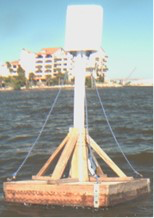
\includegraphics[width=\textwidth]{Images/SDR_bright.png}
        \caption{SDR visual camera (5 MP)}
        \label{fig:SDR_bright}
    \end{subfigure}
    \hspace{2em} % horizontal spacing between them
    \begin{subfigure}[t]{0.378\textwidth}
        \centering
        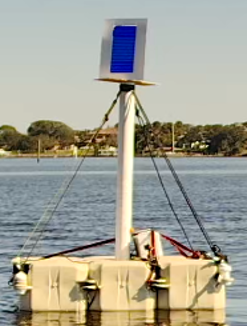
\includegraphics[width=\textwidth]{Images/HDR_bright.png}
        \caption{HDR visual camera (5 MP)}
        \label{fig:HDR_bright}
    \end{subfigure}%
}
\caption{\textcolor{red}{place-holder image – A visual comparison of the \ac{SDR} FLIR 4k camera (left) and the \ac{HDR} Leopard Imaging camera (right) in low-light conditions.}}
\label{fig:HDR_compare}
\end{figure}

In contrast, the Leopard Imaging \ac{HDR} camera offers slightly lower image resolution at a comparable effective focal length but provides substantially greater dynamic range.
% enabling detail preservation across bright and shaded regions within the same frame.  
This wider dynamic range enables more consistent color fidelity and image contrast under suboptimal lighting conditions, as illustrated in Figure~\ref{fig:HDR_compare}.

% Many tasks in the 2024 Maritime RobotX Challenge required \acp{USV} to accurately distinguish object colors as part of their operational decision-making.
This capability motivated the selection of the \ac{HDR} camera as Minion's primary visual camera sensor for the 2024 Maritime RobotX Challenge, which included several tasks that required \acp{USV} to accurately identify object colors in order to make operational decisions.
\textcolor{blue}{Check these results again}\textcolor{blue}{A comparative study by Liebergall et al.~\cite{liebergall} further supported this decision, as preliminary results indicated improved object detection results with data from the \ac{HDR} over the FLIR \ac{SDR} camera.}
Because the data collected during that competition formed the foundation of this dissertation, the Leopard Imaging \ac{HDR} camera, the primary visual spectrum sensor, was selected for all research presented in this paper.

% For these reasons, the \ac{HDR} camera was designated as the primary forward-facing visual spectrum sensor for the \ac{LiDAR}-camera fusion research presented in this paper.  




%%%%%%%%%%%%%%%%%%%%%%%%%%%%%%%%%%%%%%%%%%%%%%%%%%%%%%%%%%%%%%%%%%%%
%%%%%%%%%%%%%%%%%%%%%%%%%%%%%%%%%%%%%%%%%%%%%%%%%%%%%%%%%%%%%%%%%%%%

\subsection{PinPoint GPS/INS} \label{sensors_GPS}

% The Minion platform features a PinPoint \ac{GPS}/\ac{INS} equipped with dual-antennae for orientation and differential corrections for millimeter precision geolocation.
% The sensor performs two critical functions for the \ac{USV}: tracking vessel position and orientation, and precise global time for sensor synchronization.
% The \ac{GPS} receiver functions as the master clock for the entire synchronization hierarchy described in ~\ref{time_sync}, while the integrated \ac{IMU} enables high-rate pose updates between \ac{GPS} fixes.

The Minion \ac{USV} employs a Torc Robotics Pinpoint \ac{GPS}/\ac{INS} unit for both global positioning and inertial navigation capabilities.
This device integrates a differential-corrected \ac{GPS} receiver with a multi-axis \ac{IMU} and dual antenna, providing precise position, velocity, and orientation data for the autonomous platform.
The \ac{GPS} receiver is configured to operate at an update rate of five Hz, while the integrated \ac{IMU} provides high-frequency inertial measurements at 105.4 Hz.
The Pinpoint unit delivers timing accuracy on the order of 10-100 nanoseconds for \ac{GPS}-disciplined time signals, which is a critical function for multi-sensor synchronization discussed in Section~\ref{time_sync}.
% The device interfaces with the vessel's compute infrastructure via Ethernet, configured at IP address 201.7.90.30 on the local network.
% Beyond navigation, the Pinpoint unit serves dual roles: providing a high-accuracy time reference for sensor synchronization and delivering six-degree-of-freedom pose estimates through onboard sensor fusion algorithms.
% The specific methodologies for temporal calibration and synchronization using this device are detailed in Section 3.2.2.1, while the spatial calibration procedures appear in Section 3.2.3.


% Global Navigation Satellite System signals inherently carry highly accurate timing information, as satellite positioning operates through precise measurement of signal delay from multiple satellites with synchronized atomic clocks.
% The PinPoint receiver extracts this timing information and distributes it over the vessel's network using Network Time Protocol.
% The \ac{GPS} unit was assigned a static IP address of 201.7.90.30 on the Minion network and configured to broadcast \ac{GPS}-disciplined time via Network Time Protocol.
% The Atlas PC main computer synchronizes its clock to this \ac{GPS} source with typical accuracy in the tens to hundreds of nanoseconds, limited primarily by network latency rather than \ac{GPS} accuracy.

% This \ac{GPS} time reference propagates through the synchronization hierarchy to every computing resource on the platform.
% Atlas functions as a Network Time Protocol server for the NVIDIA Jetson Xavier camera computer, which subsequently operates as a Precision Time Protocol master for the Livox Horizon \ac{LiDAR} sensors.
% This cascaded approach ensures timestamps from all sensors—cameras, \ac{LiDAR}, and \ac{GPS}/\ac{IMU}—share a common time reference traceable to \ac{GPS} time.

% Beyond timekeeping, the \ac{GPS}/\ac{IMU} system continuously tracks platform position and orientation, which is required for \ac{LiDAR} temporal aggregation.
% As described in Section 3.1.1.3, accumulating \ac{LiDAR} points over several seconds necessitates compensation for vessel motion during that period.
% The PinPoint system fuses \ac{GPS} position measurements with \ac{IMU} acceleration and rotation data through an Extended Kalman Filter to produce pose estimates at rates substantially higher than \ac{GPS} alone could provide.
% \ac{GPS} fixes arrive at 1-10 Hz depending on satellite visibility, while the \ac{IMU} operates at hundreds of hertz.
% The fusion algorithm propagates pose estimates forward using \ac{IMU} integration between \ac{GPS} updates, subsequently correcting accumulated drift when new \ac{GPS} measurements arrive.

% The resulting pose solution provides six-degree-of-freedom state estimates—three-dimensional position and three-dimensional orientation—at sufficient temporal resolution to interpolate platform pose to the exact timestamp of each \ac{LiDAR} point.
% This capability supports the transformation methodology presented in Chapter 5, where \ac{LiDAR} points acquired at different times during motion are transformed to a common reference frame before projection onto camera images.

% The PinPoint \ac{GPS}/\ac{IMU} connects to the Minion computing infrastructure via Ethernet, utilizing both Network Time Protocol for time distribution and User Datagram Protocol for pose data transmission.
% \ac{ROS} driver nodes on the Atlas PC receive and parse the binary \ac{GPS}/\ac{IMU} messages, publishing pose estimates as standard \ac{ROS} geometry messages.
% These messages incorporate position (latitude, longitude, altitude), orientation (roll, pitch, yaw), uncertainty estimates, and \ac{GPS} fix quality flags.
% The \ac{ROS} tf2 library consumes these pose estimates to maintain the time-varying transformation tree relating sensor frames to platform and world frames, enabling automated coordinate transformation for sensor fusion.

% The \ac{GPS}/\ac{IMU} defines the local reference frame for the platform \texttt{base\_link}, with position expressed in geographic coordinates (WGS84 datum) and orientation relative to true north and local gravity.
% This world-referenced system serves as the common reference for transforming observations from multiple sensors acquired at different times during motion.
% Transformation from sensor-local frames to the \ac{GPS}/\ac{IMU} world frame requires knowledge of sensor-to-platform extrinsic calibration parameters.
% These parameters are determined through calibration procedures described in Section 3.2.1.2 for cameras and Section 3.2.1.3 for \ac{LiDAR} sensors.
% With extrinsic parameters established, the \ac{GPS}/\ac{IMU} pose solution enables transformation of any sensor observation to world coordinates or to any other sensor's reference frame.

% Maritime environments present challenges for \ac{GPS}/\ac{IMU} systems that differ from land vehicle applications.
% Water surface reflections induce multipath interference in \ac{GPS} signals, while vessel pitch and roll motion exercises the full range of the \ac{IMU}.
% The PinPoint system was designed for marine applications and incorporates algorithms to address these factors while maintaining accuracy during vessel maneuvering.
% \ac{GPS} accuracy degrades in areas with limited satellite visibility, such as proximity to tall structures, bridges, or fjord-like coastal terrain.
% The \ac{IMU} provides short-term pose continuity during \ac{GPS} outages, though accumulated drift limits the duration for which pure inertial navigation remains accurate.
% Data collection operations were conducted in open water with favorable satellite visibility, ensuring consistent \ac{GPS} fix quality throughout recording sessions.

% The \ac{GPS}/\ac{IMU} system enables two functions essential for multi-modal sensor fusion research.
% First, \ac{GPS}-disciplined time distributed to all sensors ensures timestamps from cameras, \ac{LiDAR}, and \ac{GPS} itself reference the same time base, providing frame-accurate temporal association across modalities.
% Second, continuous pose estimates enable transformation of temporally distributed observations to common reference frames, supporting \ac{LiDAR} aggregation during motion and registration of sensor fields of view for fusion operations.
% Combined with the synchronization verification and drift correction procedures described in Section 3.2.2, these capabilities establish the temporal and spatial foundation for rigorous object detection performance evaluation across sensing modalities.
% The \ac{GPS}/\ac{IMU} thus functions not merely as a navigation sensor but as critical infrastructure enabling the multi-modal perception analysis central to this research.

%%%%%%%%%%%%%%%%%%%%%%%%%%%%%%%%%%%%%%%%%%%%%%%%%%%%%%%%%%%%%%%%%%%%
%%%%%%%%%%%%%%%%%%%%%%%%%%%%%%%%%%%%%%%%%%%%%%%%%%%%%%%%%%%%%%%%%%%%
\section{Compute Hardware and Network} \label{sec:Atlas_LAN}

The Minion autonomous surface vessel employs a distributed computing architecture that balances real-time processing requirements with operational flexibility and redundancy. 
The computing infrastructure consists of high-performance workstation computers serving as the primary processing platforms, an embedded computer integrated with the camera sensors for video encoding and streaming, and a \ac{GbE} \ac{LAN} connecting all systems and sensors. 
% This architecture distributes computational workloads according to sensor proximity and processing requirements while maintaining centralized coordination through the Robot Operating System middleware. 
The following subsections detail the hardware specifications, system architecture, and network infrastructure that enable real-time multi-modal perception for maritime object detection and sensor fusion.

%%%%%%%%%%%%%%%%%%%%%%%%%%%%%%%%%%%%%%%%%%%%%%%%%%%%%%%%%%%%%%%%%%%%
\subsection{Atlas} \label{atlas}

The primary computing infrastructure consists of two identical high-performance workstation computers, designated Minion A and Minion B.  
Built with enterprise-grade components, these systems provide the computational resources required for real-time sensor processing, object detection, and autonomous navigation.  
The dual-computer configuration enables parallel software development and operational redundancy, allowing one system to operate while the other supports testing or serves as a backup.
 
Minion A, was configured with Ubuntu 22.04 for the development and migration of Minion's software to ROS 2 Humble. 
Minion B ran Ubuntu 20.04 LTS with ROS 1 Noetic, and was the only device used for data-recording and object-detection processing performed for the research of this dissertation.

% While ROS manages sensor data and transforms between reference frames, the focus in this section relates to the underlying hardware responsible for real-time, multi-modal perception.  
% The object-detection methods described in Chapter \ref{realtime_object_detection} are optimized for the computational characteristics of the CPU and GPU.  
% This distribution of processing responsibilities balances throughput, latency, and efficiency across the perception pipeline.  
% The following subsections describe how LiDAR and vision workloads are allocated between the CPU and GPU on the Atlas platform.

% While the ROS middleware manages communication and synchronization between sensor nodes, the emphasis here is on the computational workload executed by the Atlas hardware. 

% Perception processing is divided between CPU and GPU resources according to the characteristics of each object detection method.  
% LiDAR-based object detection, is performed on the CPU due to its reliance on irregular memory access patterns and control flow.  
% Conversely, vision-based detection utilizes parallel tensor operations that the GPU hardware is optimized for.  
% This allocation of workloads balances computational throughput and latency, ensuring reliable multi-modal perception and sensor fusion for autonomous operation.

% primarily between the CPU and GPU according to algorithm characteristics and hardware acceleration capabilities.

% have different workload requirements, and therefore operate primarily on separate processing units.
% Perception workloads are 
% This 
% While \ac{ROS} manages coordination and communication across processes, the following overview focuses on the hardware-level execution of LiDAR and vision tasks.

\subsubsection{CPU and Memory}
Each Atlas PC is equipped with computing hardware selected to meet the demanding real-time requirements of multimodal perception and autonomous operation.  
Table~\ref{table:Minion_hardware} summarizes the key system specifications.

The Intel Xeon processor provides six cores and a total of twelve parallel threads, allowing multiple perception and navigation processes to run concurrently.  
Tasks that require low-latency responses—such as LiDAR point cloud filtering and sensor updates benefit from the processor’s strong single-thread performance.
% , which minimizes delay between sensor input and system response.  
At the same time, the multi-core architecture supports parallel execution of computationally intensive workloads.
% , including feature extraction and classification across multiple LiDAR streams.  
Hardware vector acceleration further enhances numerical operations common to point cloud transformations and coordinate frame calculations.

The system’s 16~GB of high-bandwidth memory provides sufficient capacity to buffer LiDAR point clouds, video imagery, and other sensor data during real-time processing.  
This configuration allows multiple perception modules to access and update shared data concurrently without slowing overall system performance.

\begin{table}[htpb]
\centering
\begin{tabular}{ll}
\hline
\multicolumn{2}{c}{Minion PC - Hardware Specification} \\
\hline
\hline
Processor (CPU) & Intel Xeon E5-1650 v3 \\
CPU Cores & 6-core / 12-thread, 3.50 GHz \\
Graphics (GPU) & NVIDIA GeForce GTX 1080 \\
GPU Memory & 8 GB GDDR5X, 2560 CUDA cores \\
Memory (RAM) & (4x) 4 GB DDR4 \\
Storage (Primary) & 500 GB NVMe SSD \\
Network Interface & (6x) Gigabit Ethernet \\% + 802.11ac WiFi \\
\hline
\end{tabular}
\caption{Minion A/B PC Hardware Specifications}
\label{table:Minion_hardware}
\end{table}

\subsubsection{GPU}

The NVIDIA GTX~1080 graphics processor accelerates the vision-based object detection pipeline by handling tasks that benefit from highly parallel computation.  
Its primary responsibilities include decoding the incoming video streams from the camera enclosure and performing the image convolution operations required for vision-based detection.  
The GPUs have hardware-accelerated video encoders and decoders for processing multiple video streams, and object-detection algorithm was written to leverage the 2,560 CUDA cores for fast tensor and matrix computations and image convolution.
This also offloads H.264 decompression from the CPU, allowing the system to process multiple high-resolution camera streams simultaneously while preserving CPU resources for LiDAR and sensor-fusion tasks.

  
These operations are executed directly in GPU memory, leveraging  cores  the repetitive tensor and matrix computations common to neural network inference.  
This hardware acceleration enables real-time image processing and object detection performance that would otherwise be infeasible on CPU resources alone.

The NVIDIA GTX 1080 GPU features 2560 CUDA cores based on the Pascal architecture and 8 GB of GDDR5X memory, accelerating both machine learning inference for object detection and point cloud processing operations.
The Pascal architecture provides CUDA compute capability 6.1, enabling efficient execution of YOLOv8 convolutional neural networks and GPU-accelerated image preprocessing described in Chapter \ref{realtime_object_detection}.
Hardware video decode engines offload H.264 video decompression from the CPU, enabling the Atlas PC to receive and process multiple camera streams simultaneously while maintaining CPU resources for perception algorithms.

\subsubsection{Workload Allocation}

The CPU-GPU task distribution reflects algorithm characteristics and hardware capabilities.
LiDAR processing with irregular spatial queries and dynamic data structures exploits CPU cache hierarchies and branch prediction, while vision processing with regular tensor operations and data parallelism leverages GPU throughput.
The 6-core CPU handles approximately 3× simultaneous LiDAR processing streams plus sensor fusion logic without saturating computational resources, while the 2560-core GPU processes vision workloads that would overwhelm CPU execution.

This balanced allocation maintains real-time performance with sub-100 millisecond end-to-end latency from sensor observation to fused detection output, meeting the temporal requirements for autonomous navigation decision-making.
Load monitoring during typical operations indicates approximately 60-70\% CPU utilization across all cores and 70-80\% GPU utilization during simultaneous LiDAR and vision processing, providing margin for computational bursts during high-complexity scenes.

% \paragraph{CPU-Based Processing}

LiDAR point cloud processing and LiDAR-based object detection are executed on the system’s multi-core CPU.
These algorithms involve spatial clustering, coordinate transformations, and probabilistic data association—operations that rely on irregular memory access patterns and branching logic.
Such workloads benefit from the CPU’s high single-threaded performance, cache hierarchy, and flexible memory management.
The CPU also performs sensor fusion between LiDAR and vision detections, as well as general system coordination tasks such as recording data. %, network management, and operator interface control.

% \paragraph{GPU-Based Processing}

The GPU accelerates two perception tasks that exhibit a high degree of data parallelism: video decoding and deep learning inference.
Its first responsibility is processing video streams received from the camera enclosure. 
Video decoding and image preprocessing are performed directly in GPU memory, minimizing data transfer overhead and reducing end-to-end latency.
The second responsibility is image-based object detection using the \ac{YOLO} framework. 
This algorithm relies on convolutional and tensor operations within neural networks and is implemented to leverage the parallel processing capabilities of NVIDIA’s CUDA architecture.

\subsubsection{Storage Media}

High-speed solid-state storage provides the throughput required to record multiple sensor streams during data collection operations.
Each recording session captures raw \ac{LiDAR} point cloud data, uncompressed video imagery, GPS/INS pose information, and mapped object-detection results, producing aggregate data rates that can easily exceed 200 \ac{MBps}.
A solid-state NVMe hard drive is used on each Minion system to provide the data throughput that these operations require, and is much more robust to the motion experienced in choppy surf and vibrations experienced while in transport on the \ac{USV}'s trailer.
% and 5–15MBps per camera for H.265-compressed video at 10~fps, with additional low-bandwidth streams for GPS/INS and detection results.
% The NVMe solid-state drives provide sufficient sequential throughput and IOPS to maintain these rates for extended sessions without frame loss or buffer overflow.

% \textcolor{red}{If time allows, it may be worth mentioning the cooling system.}

%%%%%%%%%%%%%%%%%%%%%%%%%%%%%%%%%%%%%%%%%%%%%%%%%%%%%%%%%%%%%%%%%%%%
\subsection{Camera Enclosure} \label{comp:camera_enclosure}

% # Camera Enclosure Computing Platform

% for the RobotX competition in 2022, as well as the PhD research of D. Thompson \cite{thompson2023}.
% Specialized computing hardware is required to manage up to six video streams from the cameras within the enclosure.
% The camera enclosure assembly integrates six camera sensors with dedicated computing hardware housed in a weatherproof enclosure mounted on the vessel's superstructure. 


% real-time H.264/H.265 video encoding, manages timestamp embedding for temporal synchronization, and serves critical time distribution functions within the hierarchical clock architecture. This distributed computing approach places video processing at the camera location rather than transmitting raw uncompressed video over the network, substantially reducing bandwidth requirements while enabling sophisticated in-stream timestamp embedding.




The camera enclosure houses six cameras and serves as the mount for the three forward Livox LiDAR units, and was designed to be a self-contained perception platform for any maritime vessel or ground vehicle. 
Integrated into this subsystem is a compact and capable PC designed for video processing, as well as other robotics applications.
The NVIDIA Jetson AGX Xavier is designed for edge AI and computer vision applications, combining ARM-based CPU cores with a powerful GPU architecture optimized for machine learning inference and media encoding. 
The system-on-module (SOM) design integrates a processor, GPU, and memory in a compact form factor designed for speed and power efficiency.
Table \ref{table:Xavier_hardware} provides key hardware specifications.


\begin{table}[htpb]
\centering
\begin{tabular}{ll}
\hline
\multicolumn{2}{c}{NVIDIA Jetson AGX Xavier} \\
\hline
% \textbf{Component} & \textbf{Specification} \\
\hline
Processor (CPU) & 64-bit 8-core NVIDIA Carmel \\
Graphics (Integrated) & 512-core NVIDIA Volta \\
Memory (RAM) & 32 GB LPDDR4X \\
Storage (Primary) & 32 GB eMMC 5.1 \\
Storage (Secondary) & 500 GB NVMe \\
Network Interface & Gigabit Ethernet \\
Operating System & Ubuntu 18.04 LTS (Linux for Tegra / JetPack 4.x) \\
\hline
\end{tabular}
\caption{NVIDIA Jetson Xavier - Hardware and Operating System Specifications}
\label{table:Xavier_hardware}
\end{table}

% ## NVIDIA Jetson Xavier Platform
The 8-core ARM processor provides sufficient computational capacity for multiple video pipelines, network protocol handling, and system services. 
The 512-core Volta GPU supports hardware-accelerated video encoding, necessary for streaming simultaneous high-resolution video streams.
The unified memory architecture shared between CPU and GPU facilitates high-throughput data exchange for media processing pipelines.

% \subsubsection{Video Processing Architecture}
The primary computational responsibility of the Jetson Xavier is video encoding and transmission of video from the six cameras.
% three 4K cameras, two FLIR, and a single HDR camera feeds. 
The pipeline for each video follows a similar structure: raw video frames are received via USB 3.0, parsed by custom software, and then split into two processing branches. 
One branch is encoded in H.265 and saved locally to the Jetson's internal storage, while the other branch is down-sampled to a reduced frame rate before being streamed over the \ac{LAN} to one of the Minion PCs in Atlas.

This streaming reduction is essential to maintain reliable network performance given limited bandwidth, as discussed in Section \ref{comp:network}. 
The maximum bitrate $R_{\text{max}}$ of each stream is computed at runtime as a function of the target frame rate, frame resolution, and compression ratio, defined by

\begin{equation}
    R_{\text{max}} = N_x N_y b f
\end{equation}

where $N_x$ and $N_y$ are the image width and height in pixels, $f$ is the desired frame rate, and $b$ is the effective bits per pixel after compression.
For the HDR camera, the image resolution is $2880 \times 1860$ pixels, encoded in YUV 4:2:0 format using H.264 compression.
An empirically derived constant of $b = 0.14$ bits per pixel captures the combined effects of color subsampling and compression efficiency under typical scene conditions.
These values yield a bitrate for the HDR camera of

\begin{equation*}
    \begin{split}
        R_{\text{max}} & = (2880 \times 1860\; \text{px}) (0.14 \;\text{bits/px})(5\;\text{s}^{-1})  \\
        & \approx 3.75\; \text{Mbps}
    \end{split}
\end{equation*}

and scales linearly with frame rate.
This adaptive bitrate approach ensures that each video stream remains within the available network bandwidth while maintaining adequate visual fidelity for perception and data logging.
By default, each camera operates at 5 \ac{fps}, aligning with the data rate of other perception sensors, but this rate can be adjusted as needed. % to accommodate specific mission or testing requirements.


% Each camera stream defaults to 5 \ac{fps} to match the data rate of other perception data, but can be modified based upon need.
% This  us a default maintaining each stream below 25–30 Mbps to prevent network saturation.
% This ensures bandwidth allocation per stream remains within network limits while preserving visual fidelity.

While compressed video is streamed to Atlas, the Jetson simultaneously records each feed at its native frame rate to the onboard 500 GB solid-state NVMe drive as redundant backups. 
Each recording is saved in 120-second segments along with a corresponding \ac{CSV} file pairing every image frame with a timestamp from the system clock. 
The same system clock provides the \ac{PTP} signal used by the Livox LiDAR units. ensuring consistent temporal alignment across all sensors within the perception suite. 
Consequently, the timestamps in the recorded \ac{CSV} files are also essential for validating the synchronization of the camera and LiDAR, as discussed in Section \ref{time_sync_cam}.

% Local recording also serves diagnostic purposes, enabling comparison of locally-saved video files with network-transmitted ROS bag data to validate timestamp accuracy and detect any frame dropping or duplication during network transmission. The temporal drift analysis methodology described in Section \ref{time_sync_cam} exploits this local recording capability by comparing locally-saved video frames with network-transmitted ROS messages to quantify systematic timing offsets introduced by the encoding-transmission-decoding pipeline.


% The video encoding workflow exploits the Jetson's dedicated hardware encoding engines to achieve real-time compression of three simultaneous 2880×1860 pixel video streams. Hardware encoding offloads the computationally intensive compression operations from the CPU, enabling sustainable operation without thermal throttling during extended recording sessions. The RTSP bitrate is [INSERT bitrate formula here] dependent upon the requested stream frame rate (typically 5-15 fps).

% The compressed video streams are transmitted to the Atlas PC main computing platform via RTSP over UDP, where they are decoded and published as ROS image messages for consumption by object detection algorithms. This architecture distributes the encoding burden to the camera enclosure while centralizing detection processing on the more powerful Atlas hardware.

% A critical function performed by the Jetson Xavier is the embedding of precise system timestamps directly into the encoded video bitstream. Custom GStreamer pipeline elements inject SEI (Supplemental Enhancement Information) NAL units containing synchronized timestamps alongside encoded video frames. This in-band metadata approach ensures that timing information persists with the video data through network transmission, recording, and playback. The temporal synchronization procedures and timestamp validation methodology are detailed in Section \ref{time_sync_cam}.

% \subsubsection{Network Infrastructure Role}

% Within Minion's distributed computing architecture, the Jetson Xavier subscribes to the precise GPS clock provided by the Pinpoint.

% erves several network infrastructure functions. As described in Section \ref{time_sync_lan}, the system participates 

% in the hierarchical time distribution network that provides temporal synchronization for all platform sensors. The Jetson operates as both a client for receiving GPS-disciplined time and a server for providing high-precision timing to the LiDAR sensors.

% The Gigabit Ethernet interface connects the camera enclosure to the vessel local area network at IP address 201.7.90.147. This single network connection carries bidirectional traffic including compressed video streams, time synchronization protocols, remote administration access, and platform status monitoring. The camera enclosure may also include a secondary Ethernet switch to provide local network connectivity for the three Livox Horizon LiDAR units mounted on or near the camera mast, as detailed in Section \ref{comp:camera_enclosure}.

% \subsubsection{Local Recording Capability}


%%%%%%%%%%%%%%%%%%%%%%%%%%%%%%%%%%%%%%%%%%%%%%%%%%%%%%%%%%%%%%%%%%%%
\subsection{Network Structure} \label{comp:network}

Each device on the network is assigned a static IP address within a private subnet, allowing deterministic communication between endpoints.
Camera streams from the Jetson Xavier, point cloud data from each LiDAR sensor, and other telemetry are transmitted over the LAN to Atlas, which serves as the central computing and data aggregation hub.
Sensor data are processed locally, and results such as mapped and detected objects, motor control commands are published along with the raw data as \ac{ROS} message topics for system monitoring and data recording.

Under normal operation, the combined data throughput of all sensors remains below 15\% of the Gigabit Ethernet link capacity, leaving sufficient headroom for control traffic, \ac{PTP} synchronization, and administrative functions.
However, when \ac{ROS} data topics are broadcast across the network for visualization or debugging, bandwidth utilization can temporarily spike and saturate the network.
For this reason, ROS data is recorded locally, and admin visualization tools such as RVIZ are typically restricted to smaller topics related to object mapping and controls.
A high-level overview of network utilization is provided in Table \ref{table:network_bandwidth}.

\begin{figure}[htbp]
\centering
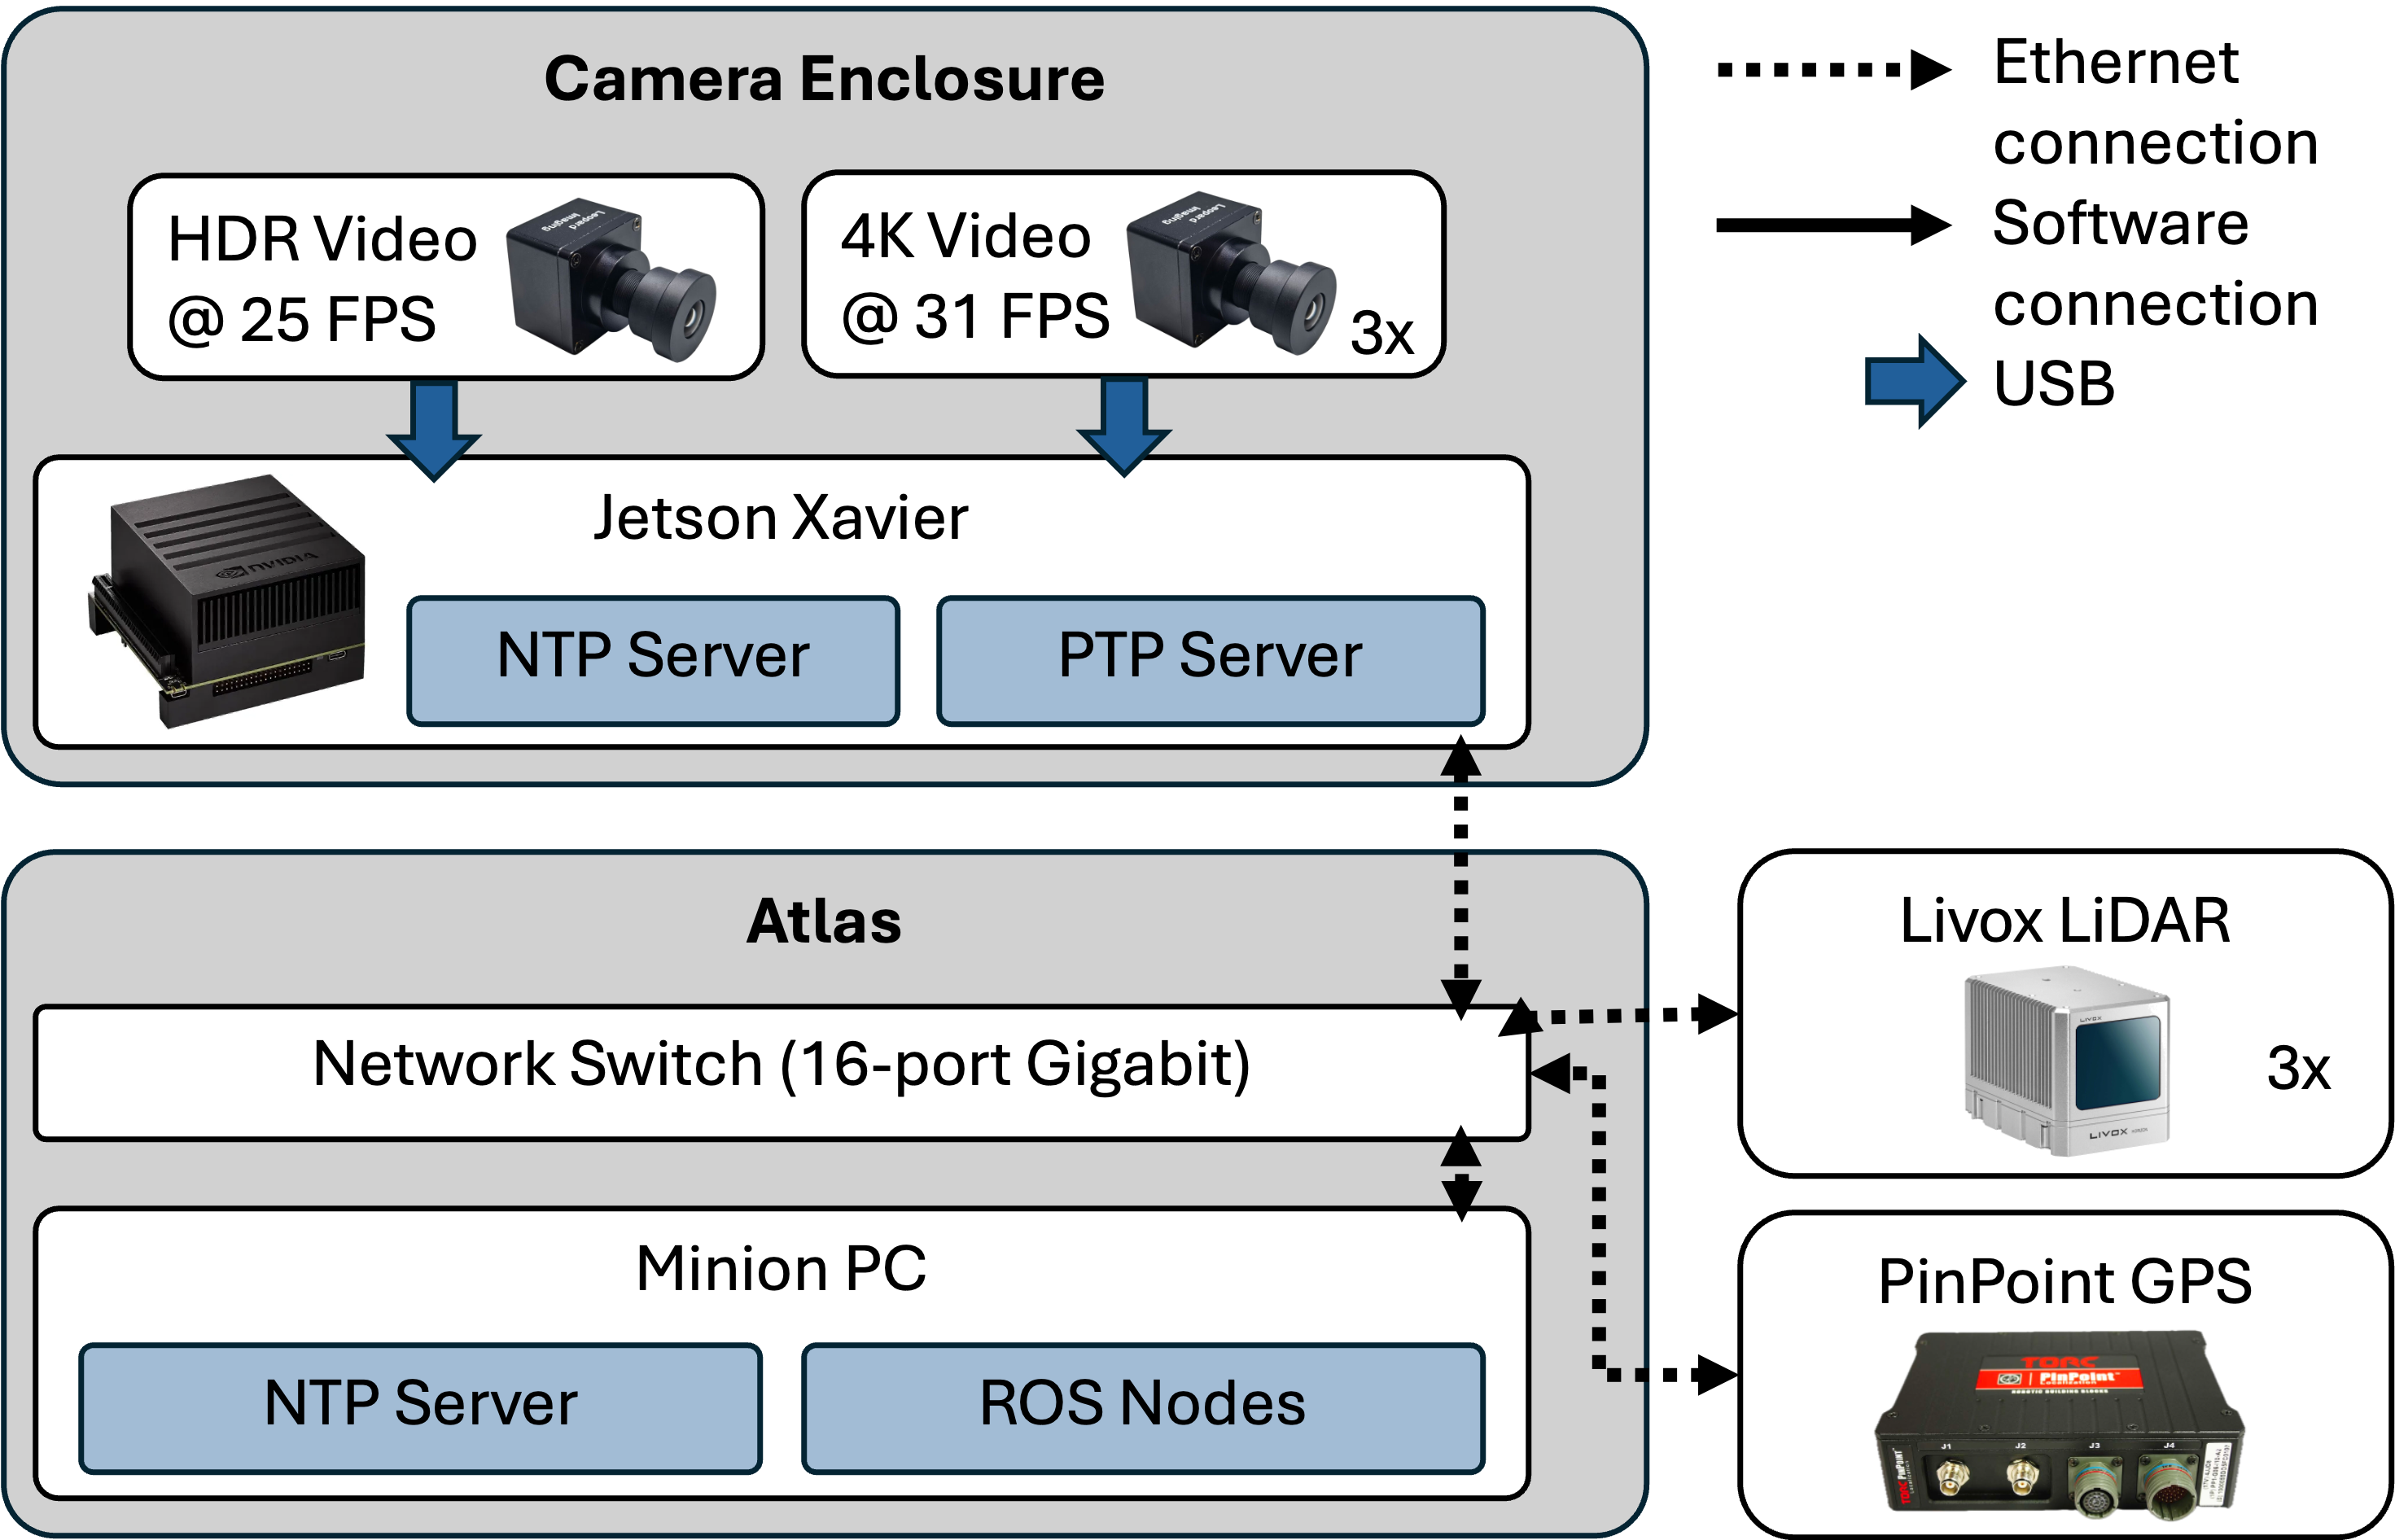
\includegraphics[width=0.8\textwidth]{Images/network_diagram2.png}
\caption{LAN diagram for Minion USV}
\label{fig:network_diagram}
\end{figure}

Although the LAN is primarily dedicated to perception and data logging, it also supports administrative access for configuration, diagnostics, and remote operation.
The Jetson Xavier is configured as a headless device and accessed remotely via Secure Shell (SSH) for camera configuration, operation, and monitoring.
Each Minion PC can be accessed through SSH, Virtual Network Computing (VNC), or Remote Desktop Protocol (RDP), enabling full graphical or terminal control for development, testing, and troubleshooting.
Network security is intentionally lightweight for field deployment, relying on standard \texttt{sudo}/root authentication and a secured wireless link protected by a strong \ac{WAN} password.
Long-range connectivity between the vessel and ground station is provided by a Ubiquiti Bullet omni-directional antenna on the \ac{USV}, paired with a directional antenna and Ubiquiti Dream Machine at the ground station, allowing administrative access without direct physical connection.




\begin{table}[htbp]
\centering
\begin{tabular}{lcc}
\hline
Data Source & Typical Bandwidth (Mbps) & \% Total Bandwidth \\
\hline
HDR Camera Stream & $3.7$--$11.2$ & $0.4$--$1.2$ \\
FLIR Camera Streams (2×) & $7.0$--$20.0$ & $0.7$--$2.1$ \\
Velodyne LiDAR Units (3x) & $43.2$--$57.6$ & $4.3$--$5.8$ \\
Livox LiDAR Units (3x) & $40.3$--$53.8$ & $4.0$--$5.4$ \\
GPS / INS Telemetry & $<0.1$ & $<0.01$ \\
Admin / SSH / Control Traffic & $0.5$--$2.0$ & $0.05$--$0.2$ \\
\hline
\textbf{Total Estimated Utilization} & \textbf{95--145 Mbps} & \textbf{9.5--14.5 \%} \\
\hline
\end{tabular}
\caption{Approximate network bandwidth utilization from direct sensor and control data sources relative to a 1 Gbps link ($\sim940$ Mbps usable).}
\label{table:network_bandwidth}
\end{table}



% The Minion autonomous surface vessel employs a dedicated Gigabit Ethernet local area network to interconnect computing platforms, sensors, and navigation equipment. 
% This network serves multiple critical functions: sensor data transmission, \ac{NTP} for system clock synchronization, and remote administration access for communication to the \ac{ROS} middleware. 
% Figure \ref{fig:network_diagram} presents a block diagram of the connected network endpoints required for sensor fusion.

% All computing platforms and sensors maintain fixed addresses throughout system operation, enabling deterministic routing and simplified network administration.




% The local network architecture connects all major perception and processing nodes within the vessel and provides a unified temporal reference across systems.
% Time synchronization is managed hierarchically through GPS, Chrony, and PTP, ensuring consistent timestamps for all recorded data streams.

% At the top of the synchronization hierarchy, the Pinpoint GPS/INS unit provides a GPS-disciplined Network Time Protocol (NTP) reference to both the Atlas PC and the Jetson Xavier via the onboard router. Each device runs the Chrony service (Ubuntu 18.04), which continuously aligns the local system clock to the GPS reference with sub-millisecond accuracy.

% \begin{figure}[htbp]
% \centering
% 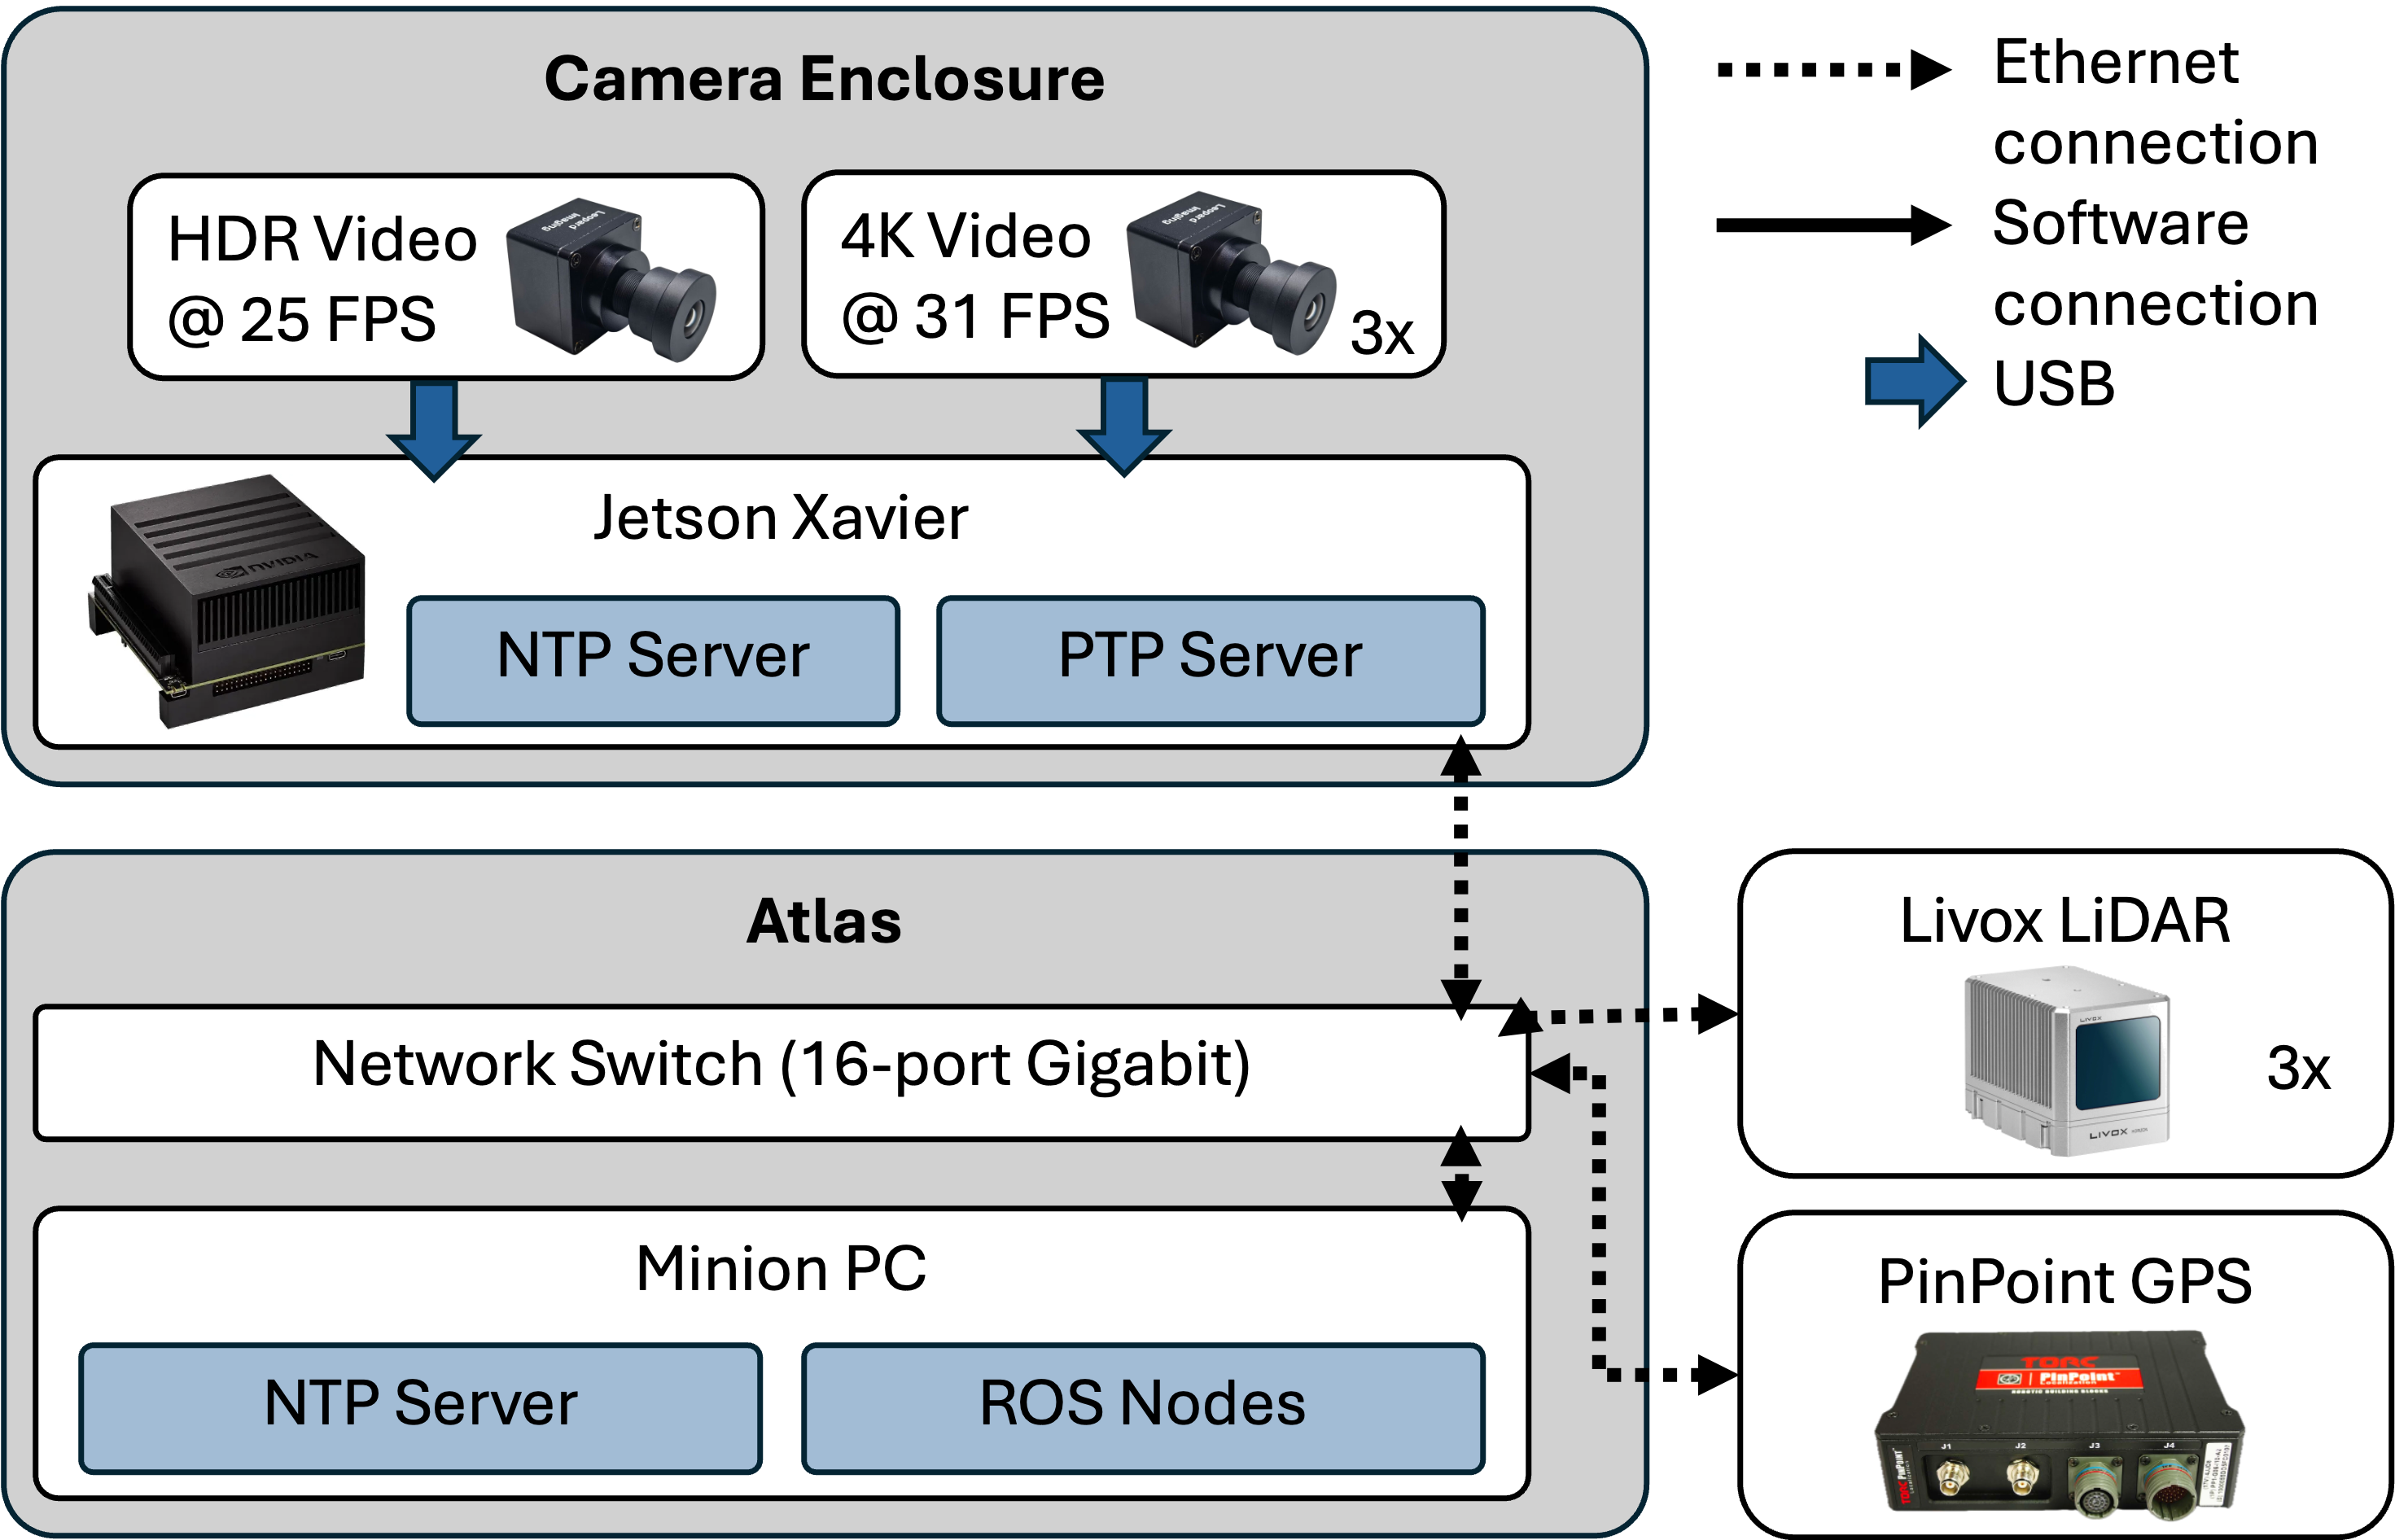
\includegraphics[width=0.8\textwidth]{Images/network_diagram2.png}
% \caption{Minion's LAN for network end-points related to real-time object detection}
% \label{fig:network_sync}
% \end{figure}

% The Jetson Xavier, serving as the core perception node, then acts as the PTP master for the Livox LiDAR units. Through the Precision Time Protocol (IEEE 1588), the Jetson broadcasts high-precision timestamps to all connected LiDAR clients, achieving microsecond-level synchronization between video and LiDAR data streams. This configuration ensures that every sensor measurement—image frame, LiDAR scan, or GPS fix—is temporally aligned to a common reference frame, enabling accurate data fusion and calibration as described in Section \ref{time_sync_cam}.

% Network bandwidth allocation is carefully managed to prevent congestion during real-time operation.
% Each Jetson video stream dynamically adjusts its bitrate based on the active frame rate, while LiDAR and telemetry traffic maintain constant low-latency channels.
% Table \ref{table:network_bandwidth} summarizes the approximate bandwidth usage across major network components.

% \begin{table}[htbp]
% \centering
% \begin{tabular}{lcc}
% \hline
% \textbf{Data Source} & \textbf{Protocol / Port} & \textbf{Typical Bandwidth (Mbps)} \\
% \hline
% HDR Camera Stream (Jetson $\rightarrow$ Atlas) & RTP / UDP & 3.7–11.2 \\
% FLIR Camera Streams (2x) & RTP / UDP & 7.0–20.0 (total) \\
% Livox LiDAR Units (3x) & UDP / PTP Client & 15.0–18.0 (total) \\
% GPS / INS Telemetry & NMEA / TCP & $< 0.1$ \\
% PTP Synchronization Packets & IEEE 1588 / UDP & $< 0.01 $\\
% \hline
% \textbf{Total Estimated Utilization} & — & \textbf{25–50 Mbp/s} \\
% \hline
% \end{tabular}
% \caption{Approximate Network Bandwidth Utilization}
% \label{table:network_bandwidth}
% \end{table}

% Security considerations for remote access include firewall configuration to restrict inbound connections, authentication requirements for SSH administrative access, and potential disconnection of external network access during sensitive operations to prevent unauthorized interference. The remote access infrastructure facilitates collaboration between multiple researchers working on different system components, as well as monitoring by shore-based personnel during extended autonomous operations.

% \subsubsection{Integration with Distributed Computing Architecture}

% The network infrastructure provides the physical medium for the distributed computing architecture that spans multiple platforms. The Jetson Xavier camera enclosure performs video encoding at the sensor location, transmitting compressed streams to the Atlas PC for object detection processing. This distribution optimizes bandwidth utilization by avoiding transmission of raw uncompressed video while maintaining centralized processing for computationally intensive algorithms.



% \subsubsection{Network Performance Validation}

% Network performance validation procedures employed during system commissioning verify that the infrastructure meets requirements for real-time perception and control. These procedures include bandwidth testing using iperf3 or similar tools to verify Gigabit link speeds between key endpoints, latency measurement via ping utilities to measure round-trip latency for time-critical paths, packet loss assessment through extended ping tests or UDP stream analysis to verify zero packet loss under load, and time synchronization quality monitoring to confirm clock accuracy meets requirements as detailed in Section \ref{time_sync_lan}.

% These validation procedures ensure that the network infrastructure meets the performance requirements necessary for real-time multi-modal perception and accurate temporal alignment of sensor data. Baseline performance metrics established during commissioning provide reference values for ongoing network health monitoring during field operations.

%%%%%%%%%%%%%%%%%%%%%%%%%%%%%%%%%%%%%%%%%%%%%%%%%%%%%%%%%%%%%%%%%%%%
%%%%%%%%%%%%%%%%%%%%%%%%%%%%%%%%%%%%%%%%%%%%%%%%%%%%%%%%%%%%%%%%%%%%
\section{Sensor Calibration} \label{sec:calibration}

% brief overview of TF_tree

%%%%%%%%%%%%%%%%%%%%%%%%%%%%%%%%%%%%%%%%%%%%%%%%%%%%%%%%%%%%%%%%%%%%
%%%%%%%%%%%%%%%%%%%%%%%%%%%%%%%%%%%%%%%%%%%%%%%%%%%%%%%%%%%%%%%%%%%%
\subsection{Temporal Calibration}\label{time_sync}

Multi-modal sensor fusion for object detection fundamentally requires accurate temporal alignment of observations from sensors operating with independent clocks and sampling at different rates.
The Minion platform employs a hierarchical temporal calibration architecture that distributes GPS-disciplined time from a single authoritative source through multiple computing platforms to all perception sensors, ensuring millisecond-level synchronization for camera observations and microsecond-level precision for LiDAR spatial measurements.
This three-tier synchronization system, employing GPS as the time authority, Network Time Protocol for coarse distribution, and IEEE 1588 Precision Time Protocol for fine synchronization, provides the temporal reference frame essential for rigorous cross-modal detection performance analysis.

The temporal calibration methodology addresses timing challenges specific to distributed embedded systems operating in maritime environments where internet connectivity is unavailable and GPS represents the sole external time reference.
Cameras and LiDAR sensors timestamp observations independently using local clocks, yet valid sensor fusion demands that all observations share a common temporal reference.
Without accurate time synchronization, a vessel traveling at 5 meters per second accumulates 5 millimeters of spatial misalignment for every millisecond of timing error, rendering temporal associations between camera frames and LiDAR scans unreliable for detection performance comparison.

The GPS-NTP-PTP cascaded synchronization architecture addresses accuracy requirements varying by sensor type.
Millisecond precision suffices for 10 Hz camera frame timestamps, while individual LiDAR laser returns require sub-millisecond accuracy to avoid spatial smearing during vehicle motion.
The hierarchical architecture exploits protocol characteristics matched to sensor needs: NTP provides simplicity and wide device compatibility for distributing time to computing platforms, while PTP achieves the microsecond-level precision demanded by spatial measurement sensors through hardware-timestamped network packets and symmetric delay compensation.

The synchronization infrastructure must accommodate operational constraints including dual redundant computing platforms requiring coordination to prevent conflicting time sources, automated startup verification to ensure synchronization establishment before data recording begins, and diagnostic capabilities enabling remote monitoring of synchronization quality during offshore operations.
Additionally, the video processing pipeline introduces systematic timing offsets between frames recorded locally on the camera enclosure computer and frames transmitted over the network to the primary computing platform, necessitating comprehensive temporal drift analysis and correction procedures to achieve frame-accurate temporal alignment.

%%%%%%%%%%%%%%%%%%%%%%%%%%%%%%%%%%%%%%%%%%%%%%%%%%%%%%%%%%%%%%%%%%%%
\subsubsection{Network Synchronization} \label{time_sync_lan}

% ## Hierarchical Clock Synchronization Architecture

The Minion autonomous surface vessel employs a three-tier time distribution hierarchy that cascades GPS-disciplined time through computing platforms using progressively more precise synchronization protocols matched to downstream accuracy requirements.

% ### GPS Time Authority

At the foundation of the synchronization hierarchy, the Torc Robotics Pinpoint GPS/INS receiver extracts UTC time from GNSS satellite signals with typical accuracy of 10-100 nanoseconds.
GPS positioning fundamentally depends on precise timing since satellite ranging measurements derive from time-of-flight calculations assuming nanosecond-accurate satellite clocks.
The receiver exploits this timing information to provide an authoritative time reference for the entire perception system, operating as a stratum-1 NTP server at IP address 201.7.90.30 on the vessel local area network.

GPS time accuracy depends on satellite constellation visibility and multipath interference.
Open-water operations with clear sky visibility typically achieve 10-50 nanosecond accuracy, though coastal operations near tall structures or in constrained waterways may experience degraded accuracy.
The GPS receiver reports fix quality indicators including satellite count and dilution of precision that enable monitoring of timing solution quality.

% ### Network Time Protocol Distribution

The first distribution tier employs Network Time Protocol to propagate GPS time from the Pinpoint receiver to the primary computing platform.
One of the two Atlas PCs executes the Chrony NTP daemon configured simultaneously in client and server modes.
As a client, Chrony synchronizes the Atlas system clock to the Pinpoint GPS.
As a server, Chrony provides NTP time to downstream platforms including the NVIDIA Jetson Xavier camera enclosure computer.
Network latency on the Gigabit Ethernet vessel LAN limits NTP synchronization accuracy to 1-10 milliseconds, an acceptable precision given the Atlas PC's role in timestamp logging and system coordination rather than direct sensor data acquisition.

Chrony represents a modern NTP implementation optimized for systems that may experience intermittent network connectivity or be started and stopped frequently.
Key advantages over the traditional ntpd daemon include rapid synchronization after startup or network outage, accuracy maintenance with intermittent reference clock availability, low-jitter operation through disciplined clock algorithms that minimize time step discontinuities, and flexible configuration supporting offline operation mode for GPS-only scenarios.

The Chrony configuration file specifies the Pinpoint GPS as the primary time source with highest priority, followed by internet NTP pool servers as fallbacks.
The configuration enables server mode, allowing the Atlas PC to respond to NTP queries from other vessel systems.

% #### Dual-Computer Coordination

A critical operational constraint arising from dual redundant Atlas PCs demands that only one system operate as the active NTP server at any time.
Multiple NTP servers providing slightly different time would cause downstream clients to experience clock instability alternating between sources.

Operational procedures specify that the active primary Atlas PC enables Chrony NTP server mode, while the standby system disables the service to prevent timing conflicts on the network.
When operators switch the active primary between Atlas PCs for software updates or failover, Chrony must be disabled on the former primary before enabling it on the new primary to maintain unambiguous time distribution.

% #### NTP Synchronization Monitoring

Chrony provides diagnostic commands for monitoring synchronization status.
The command `chronyc sources` indicates which time source is currently selected and displays reach status, delay, and offset measurements.
A healthy GPS-synchronized Atlas PC typically shows reach status of 377 octal indicating 8 consecutive successful queries, delay below 1 millisecond for local GPS source on the LAN, and offset below 10 milliseconds between local clock and GPS time.

During system validation, operators verify that the Atlas PC selects the Pinpoint GPS as the active source and achieves offset below 10 milliseconds, confirming GPS time distribution to the vessel computing infrastructure.

% ### Jetson Xavier NTP Client Configuration

The NVIDIA Jetson Xavier camera enclosure computer operates as an NTP client synchronized to the Atlas PC NTP server.
The Jetson runs Chrony in client-only mode, configured to query the Atlas PC for time updates.
The Jetson's NTP synchronization quality directly impacts video timestamp accuracy, as frame timestamps are sampled from the Jetson system clock at the moment each frame is captured from the cameras.
Network latency between the Atlas PC and Jetson typically remains sub-millisecond on the dedicated Gigabit LAN, enabling NTP synchronization accuracy of 1-5 milliseconds.

% #### Mandatory Synchronization Verification

The video encoding pipeline implements mandatory synchronization verification before launching the camera capture and encoding processes.
The startup script executes checks with defined timeouts.

The first verification confirms Chrony synchronization within a 60-second timeout, querying Chrony status to ensure leap status shows Normal rather than Not synchronized and confirming active sync with an upstream NTP source.
The second check verifies system clock update within a 30-second timeout, ensuring that the system clock timestamp reflects actual calendar time rather than a default epoch value indicating loss of synchronization or reboot without successful NTP acquisition.

Only after both verification checks pass does the startup script launch the GStreamer video encoding pipelines, preventing recording of video with uncalibrated timestamps that would compromise temporal alignment.
If synchronization verification fails within the timeout periods, the startup script reports an error and does not launch video recording, requiring operator intervention to diagnose and resolve the NTP configuration issue.

% ### Precision Time Protocol for LiDAR Synchronization

While NTP's millisecond-level accuracy suffices for video frame timestamps given the 100-millisecond frame intervals at 10 Hz capture rate, LiDAR sensors demand substantially higher timing precision.
The Livox Horizon units output point clouds at 100 Hz with each point individually timestamped.
Positioning accuracy requirements dictate sub-millisecond timestamp precision to avoid spatial errors during vehicle motion.
A vessel rotating at 10 degrees per second with LiDAR observations at 200-meter range accumulates 3.5 meters of spatial error for every 100 milliseconds of timing uncertainty, motivating the use of high-precision synchronization protocols for spatial sensors.

The Jetson Xavier, having synchronized its system clock to GPS time via NTP, operates as a PTP master clock providing microsecond-accurate synchronization to the three Livox LiDAR sensors.
The Linux PTP project's `ptp4l` daemon implementing IEEE 1588-2008, also known as PTP version 2, broadcasts PTP timing packets over the camera enclosure Ethernet network segment that includes the three Livox sensors.

% #### PTP Message Exchange Protocol

PTP operation involves periodic exchange of several message types that enable precise time synchronization.

Sync messages broadcast the timestamp of message departure from the master clock.
Follow-Up messages provide precise departure timestamps if operating in two-step mode, where hardware timestamping occurs after packet transmission begins.
Delay Request and Delay Response messages enable slave-initiated delay measurement for symmetric delay estimation, allowing slaves to measure the round-trip network delay and compensate for propagation time.
Announce messages advertise master clock quality for Best Master Clock Algorithm arbitration, enabling automatic selection of the optimal time source when multiple PTP masters are present on the network.

The Livox Horizon sensors implement PTP slave functionality, automatically discovering available PTP masters via Announce messages and synchronizing to the selected master.
In the Minion configuration, the Jetson Xavier represents the only PTP-capable device on the camera enclosure network segment, ensuring unambiguous master selection without requiring configuration of specific master IP addresses in the Livox devices.
The Best Master Clock Algorithm compares clock quality indicators from all potential masters on the network segment, though with a single master present, the algorithm simply selects the Jetson Xavier as the authoritative time source for the LiDAR sensors.

\begin{figure}[htbp]
\centering
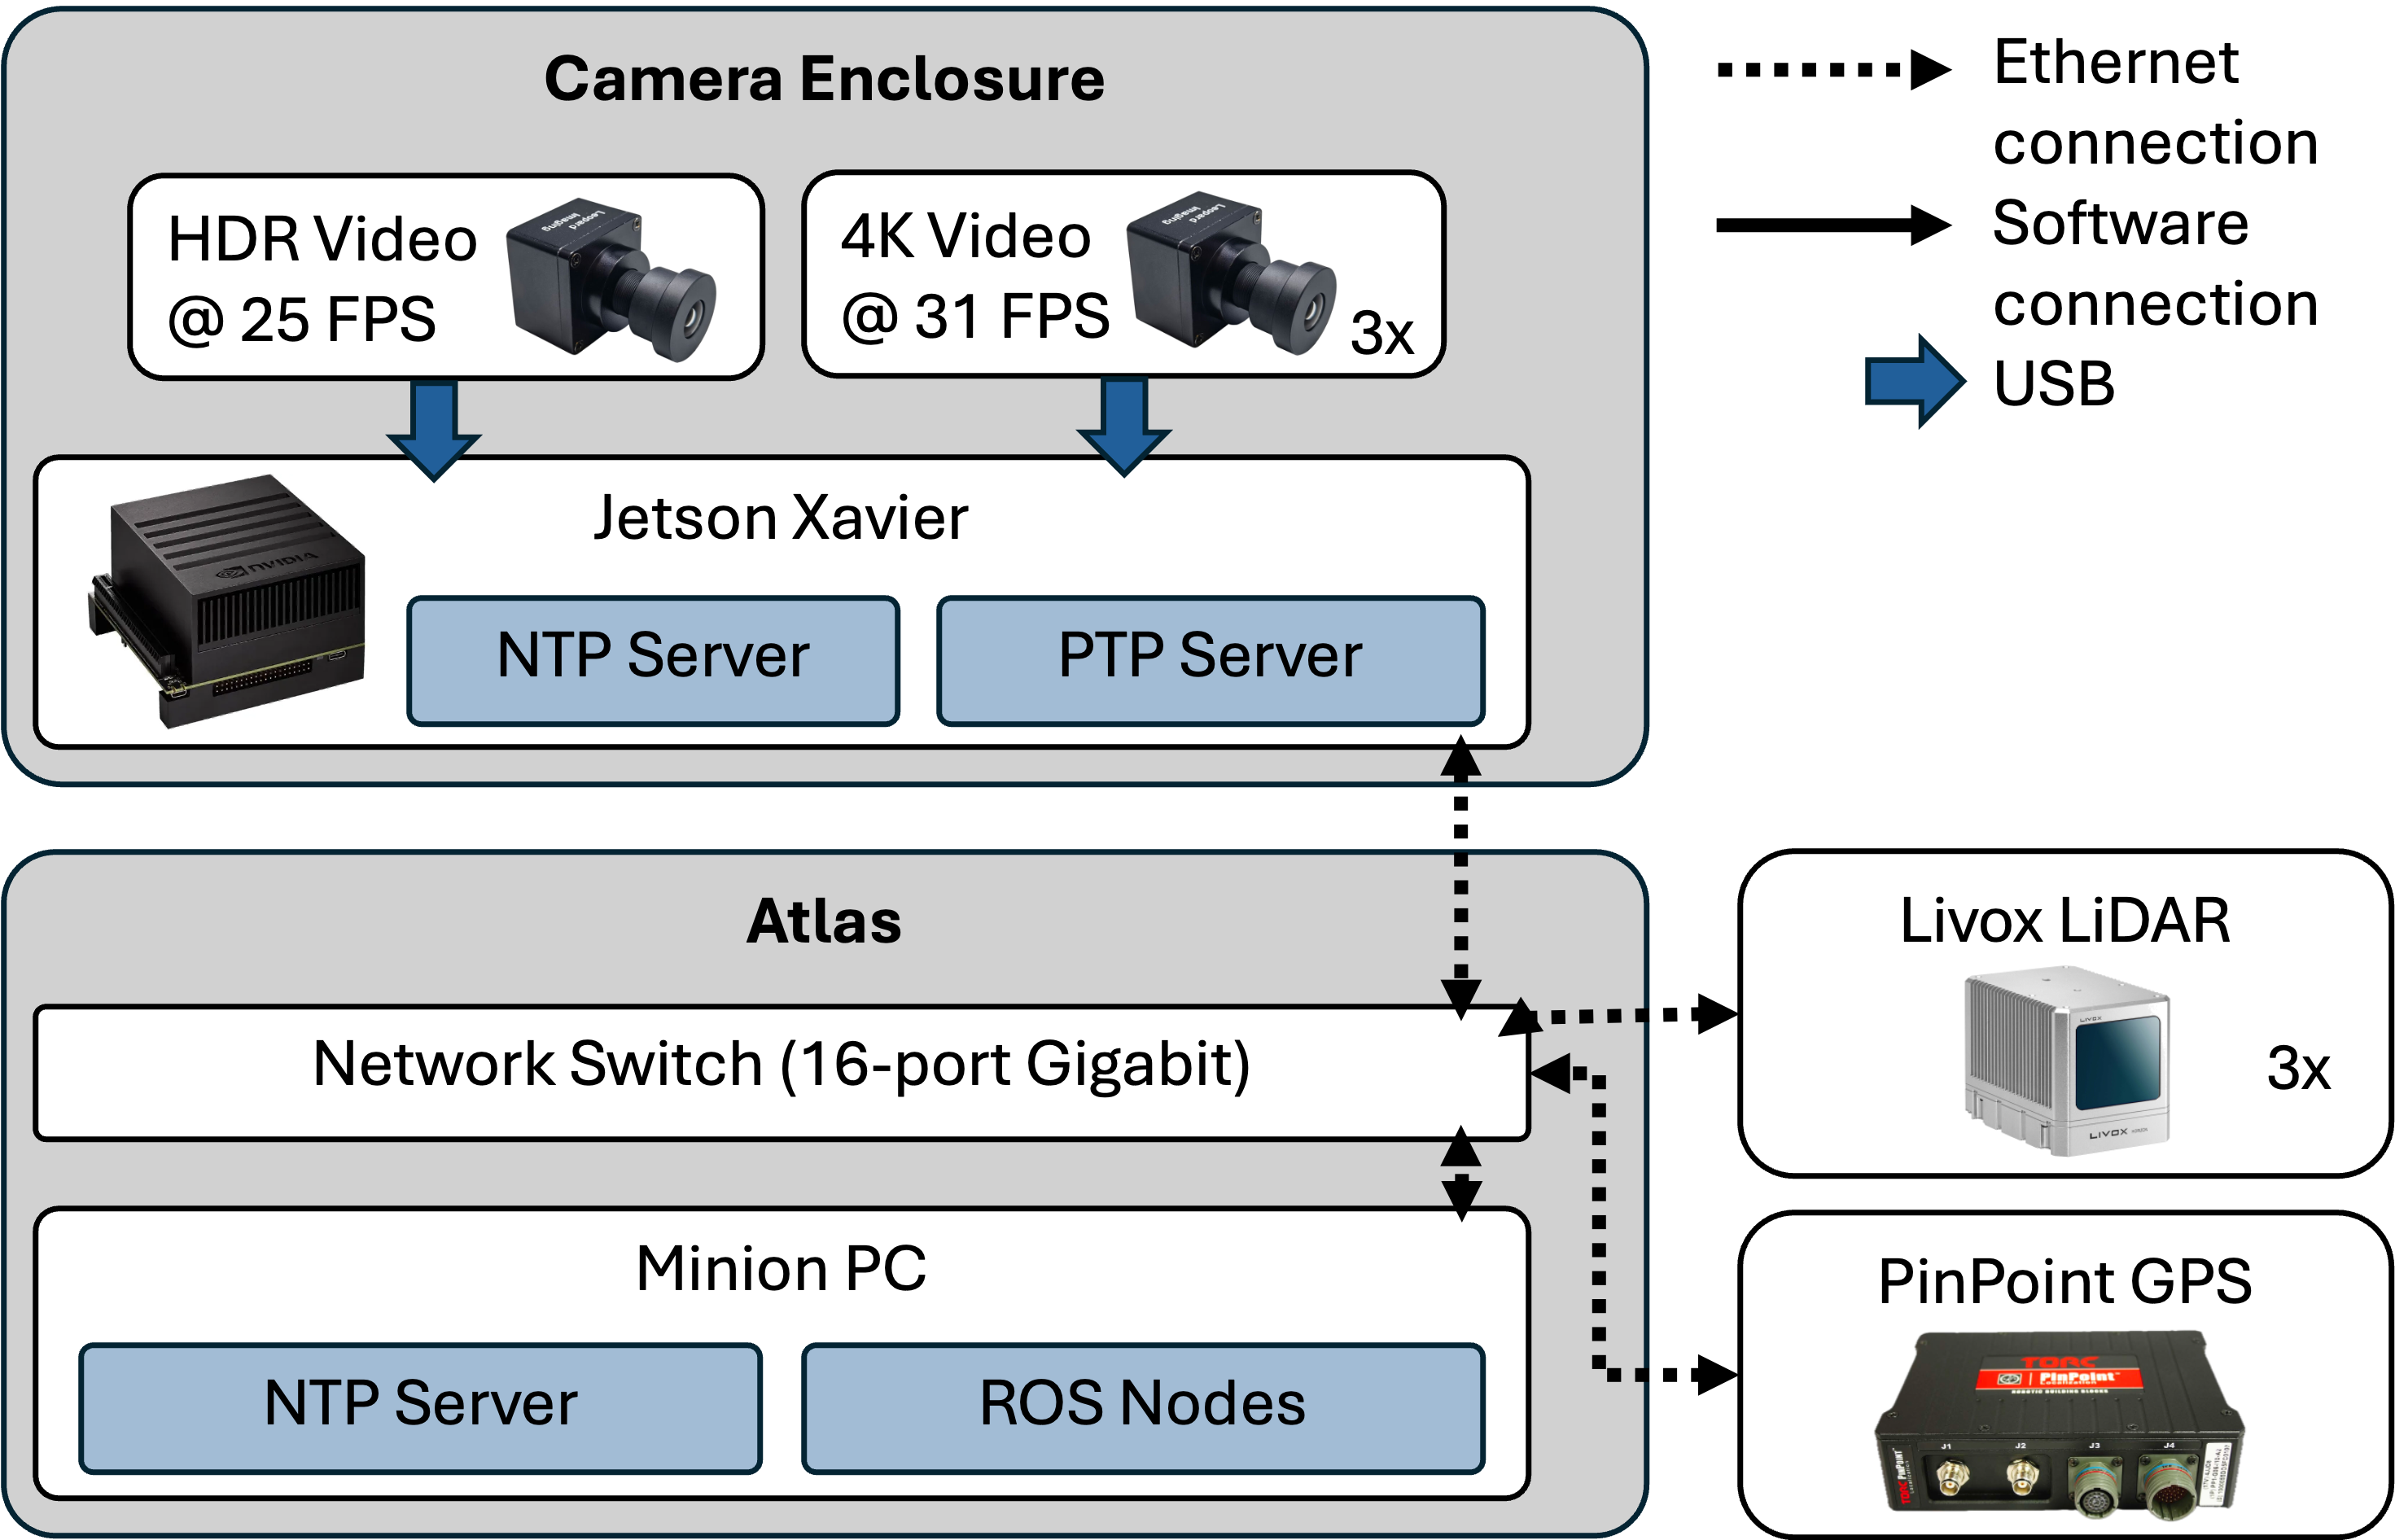
\includegraphics[width=0.8\textwidth]{Images/network_diagram2.png}
\caption{LAN diagram for Minion USV}
\label{fig:network_sync}
\end{figure}

While Minion's camera and LiDAR systems have been spatially calibrated for previous competitions, the video signal can be delayed due to inefficient encoding or network latency. 
If unaddressed, this time lag creates a temporal misalignment between the LiDAR and camera frames while the vessel is in motion.

% While Minion's vision system has been spatially calibrated for previous competitions, the timestamp for each frame in the image was estimated with a constant offset the latency. 
On Minion, object detection is performed with GB-CACHE \cite{coyleE} using LiDAR data.
Before this year's competition, any vision-based object or color detection was performed in parallel to the LiDAR-based perception. 
Video latency was addressed by adding a constant offset to the video timestamp.
While this was sufficient for tasks where the USV was stationary, such as detecting the color code sequence, the uncertainty between the time of actual and estimated image capture limited the system's use while in motion.

To remedy this, a custom script was written to record the system time whenever a new video frame was captured by the camera, and simultaneously encode this timestamp with the image frame as supplemental encoded information (SEI) in the video stream.
An additional script was written as a ROS node which decodes the video frame and timestamp and then publishes that information as a ROS message.
Figure \ref{video_pipeline} provides a block diagram of the software and hardware for this synchronization process.

%%%%%%%%%%%%%%%
% The custom "host" script which embeds the timestamps into the video stream was written in C++ and the G-streamer API.
% It uses the system clock to capture the moment each video frame is received down to the millisecond, and splits the video signal into two branches before encoding.
% The first branch is encoded at a higher bit-rate and the camera's native frame rate, and is saved locally for future use.
% The second branch is down sampled to a user-defined frame rate. This information is along with the camera's resolution to dynamically determine the optimal bit-rate for the video stream.
% Fifteen frames per second (FPS) was ultimately selected to balance the bandwidth and our data requirement of 10 FPS to provide a buffer for dropped frames.
% Hardware accelerated encoding is leveraged for both branches, enabled by the NVIDIA Jetson hardware to further reduce latency.

% % Streaming video over a network provides many standardized options for timekeeping.
% G-streamer uses the real time protocol (RTP) for transmitting video which utilizes it's own precision timing code.
% This timing code always counts up from zero
% Both the H.264 and H.265 encoding standards provide a space for custom SEI data within the header of each video frame.
% Each video frame is sliced into packets of 64 bits 
%%%%%%%%%%%%%%%


% The solution to this process was to encode a timestamp for each video frame with the system clock into the video stream.
% This solution is much more robust than using the 
% In order for video imagery to correlate with LiDAR data, the images received need to be synchronized in time with the
% Even with NVIDIA accelerated video encoding and a reduced frame-rate, the time-code for video streams need to be adjusted to account for network latency.
% It consists of six cameras (four high-definition and two thermal cameras) which connect to a compute module responsible for storing the recorded video, as well as encoding the camera data and streaming it to Minion’s local area network (LAN). Specifications for the camera enclosure hardware is provided in \textcolor{red}{TABLE123}.


% [...]
% To remedy this, a custom script was written to record the system time whenever a new video frame was captured by the camera, and simultaneously encoded this timestamp with the image as supplemental encoded information (SEI).
% [\textcolor{red}{site SEI and h.264 standards}]. 
% The full breakdown of the scripts responsible for sending and receiving the video stream is given in \textcolor{red}{Table123}.
Adopting this solution required that the system clock of the Jetson computer responsible for encoding and transmitting the video feeds from the camera enclosure is in near-perfect synchronization with Minion’s onboard PC that hosts the ROS functionality. 
This is handled in Linux with the system utility chrony, which aligns the system clock in the enclosure with Minion's main PC every time the system powers on.
It also monitors the clocks via a network time protocol (NTP) for any drift or error introduced through network traffic.


% \textcolor{red}{One major challenge in developing this custom solution was the operating system (OS) installed on the PC responsible for capturing the video. We were unable to upgrade its OS due to the legacy drivers required for the cameras installed in the enclosure, which are no longer manufactured or supported. This meant that a solution had to be built within the constraints of the installed OS, which was limited to an older version (1.14) of the video capture software GStreamer. SEI data encoding was clearly a desired feature, as it was added to subsequent releases of the GStreamer API (now on version 1.20). Furthermore, documentation and support discussion for this aging version of GStreamer was had to be found on sites which are not indexed by major search engines, or through preserved forums indexed by the way back machine [link/ref].}


This approach allows for granular customization of the video stream size, frame rate, network bit rate, and compression method. 
Additionally, because of the structure of ROS, any ROS module that needs to subscribe to the video stream is able to receive the imagery with the correct timestamp. However, to minimize network load, modules only subscribe to this stream when necessary, such as when a specific task is being conducted. 
% While open-source plugins like GSCam \cite{GSCam} and DeepStream \cite{deepstream} exist to incorporate video into ROS, Minion's solution is flexible and better adapted to address the network latency seen with Minion's specific hardware.


%%%%%%%%%%%%%%%%%%%%%%%%%%%%%%%%%%%%%%%%%%%%%%%%%%%%%%%%%%%%%%%%%%%%
\subsubsection{Camera Synchronization} \label{time_sync_cam}

\begin{figure}[ht]
\centering
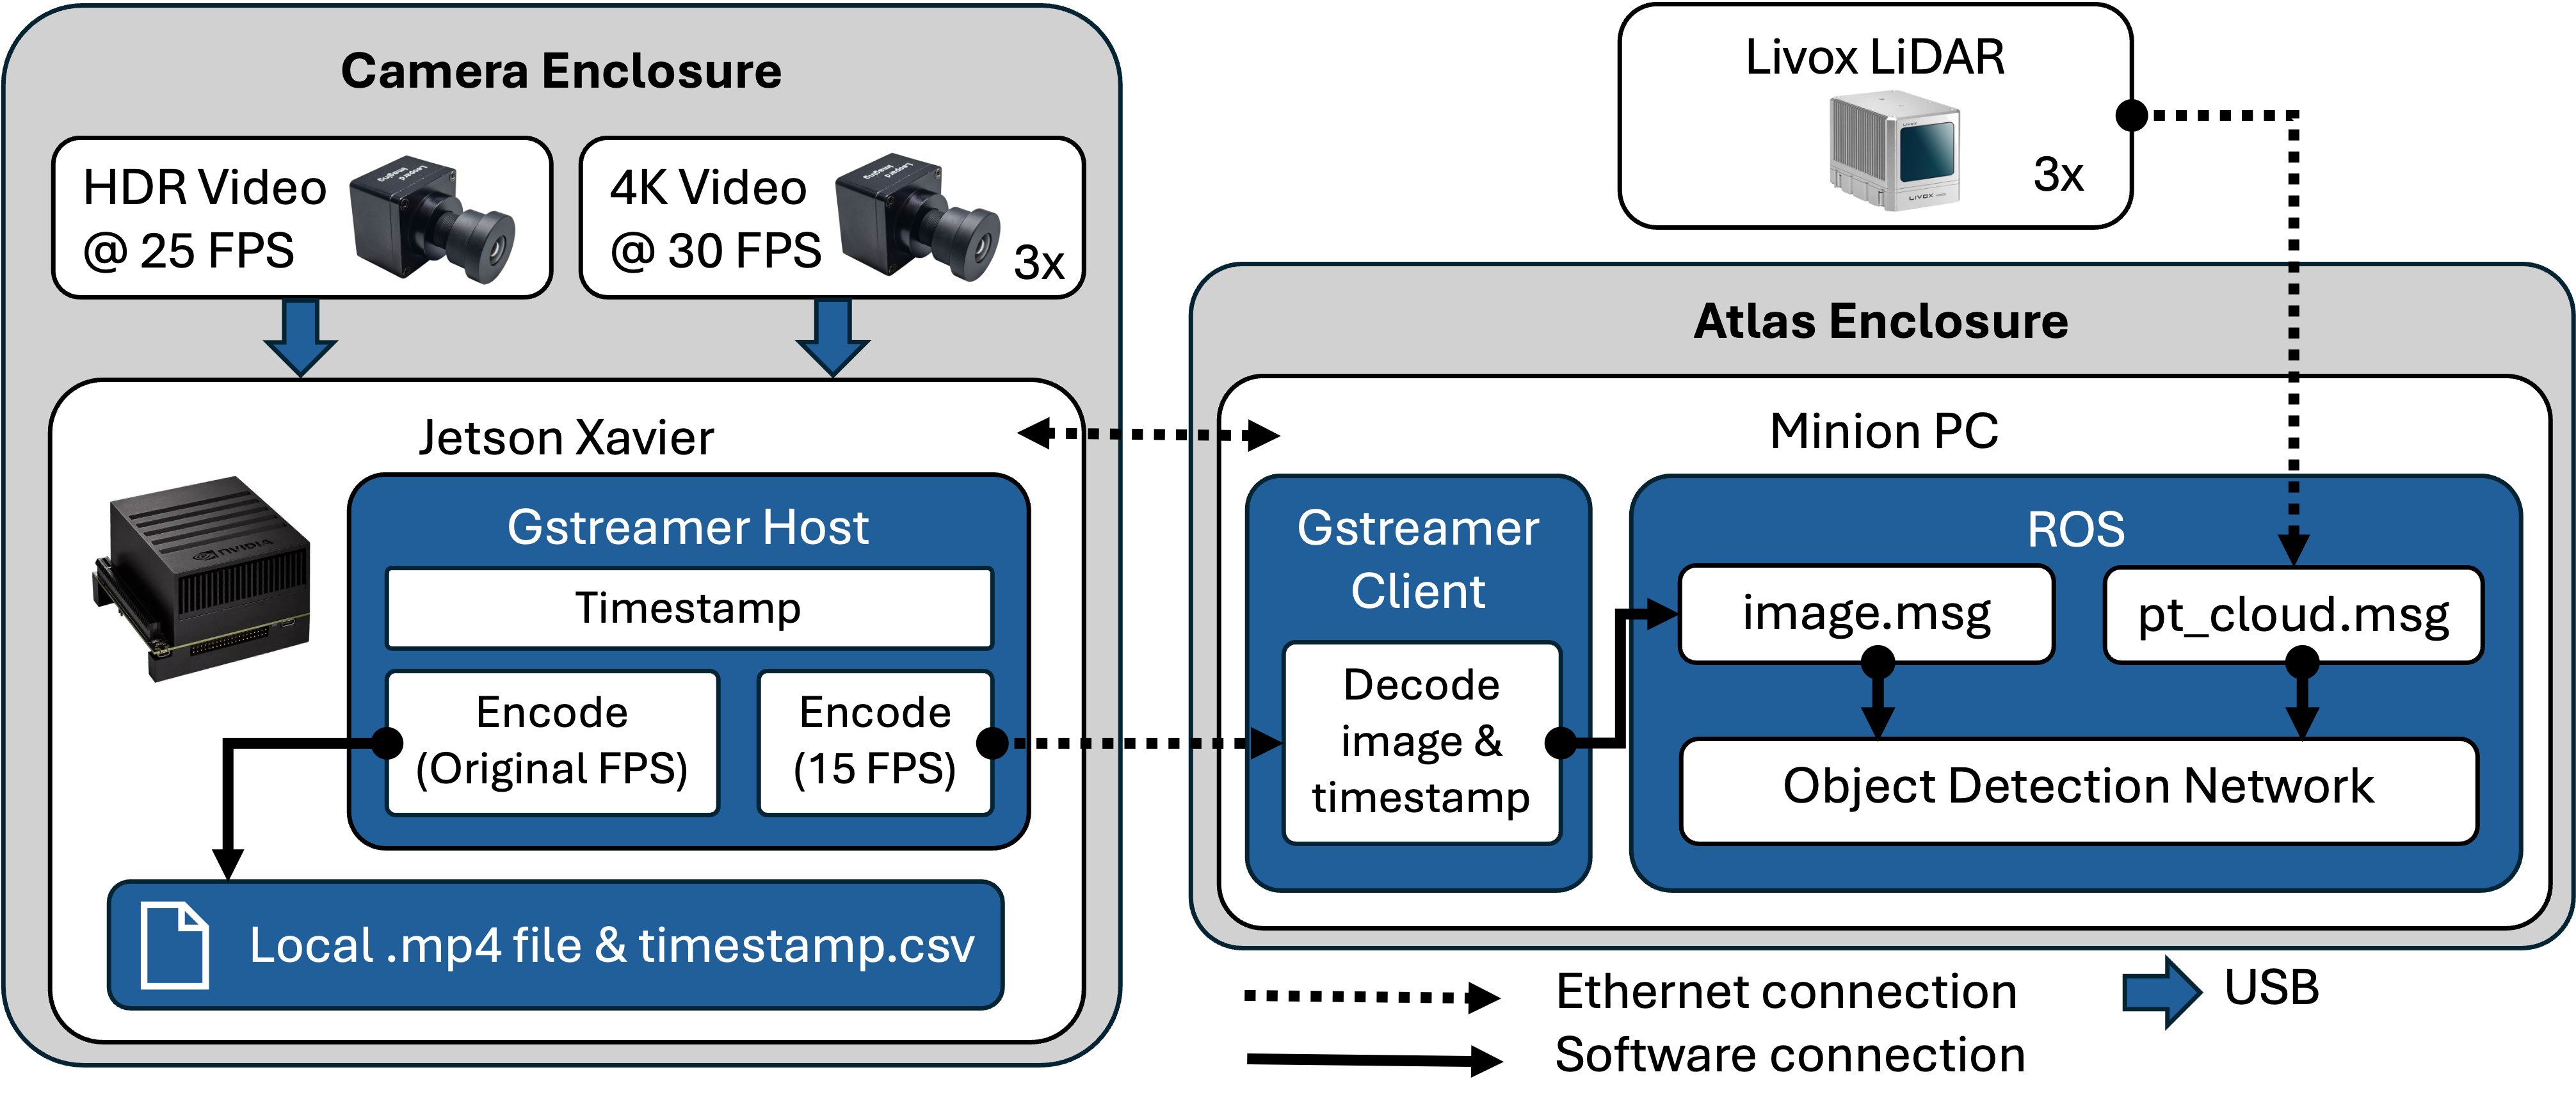
\includegraphics[width=5in]{Images/Video_Block_Diagram.png}
\caption{Block diagram of the vision system's hardware and video pipeline software.}
\label{video_pipeline}
\end{figure}

% ## Video Timestamp Embedding Methodology

Standard video processing workflows assign timestamps relative to stream start time, proving inadequate for multi-sensor fusion applications requiring absolute temporal references.
The video pipeline employs a sophisticated timestamp embedding methodology that preserves GPS-synchronized timing information through the entire video encoding, transmission, decoding, and recording chain by injecting absolute system timestamps directly into H.264/H.265 video bitstreams as Supplemental Enhancement Information metadata.
This approach ensures that timing information remains inseparably bound to corresponding video frames throughout all processing stages, representing a critical enabling technology for temporal alignment between camera observations and LiDAR point clouds.

% ### Design Requirements and Alternative Approaches

The GStreamer multimedia framework employed for video capture and encoding operates with timestamps measured from the beginning of each stream, a convention suitable for multimedia playback synchronization but incompatible with the requirement to associate video frames with LiDAR observations timestamped in GPS time.

Several approaches for associating absolute timestamps with video frames were evaluated.

External CSV logging writes frame numbers and timestamps to a separate file, requiring manual association during post-processing.
This approach fails when frames are dropped or reordered as the frame-to-timestamp association breaks.

RTP timestamp modification encodes timing in Real-Time Protocol headers used for network transmission.
However, RTP timestamps provide only relative timing, RTP headers are discarded during recording to standard video files, and RTP provides limited timestamp precision with its 90 kHz clock for video streams.

Video overlay approaches render timestamp text directly onto frames as visible graphics.
This method requires optical character recognition for automated extraction while consuming pixel area that occludes image content and increases encoding bitrate due to high-frequency text features.

In-band metadata embedding injects timestamps as structured data within the video bitstream itself via SEI NAL units.
This approach was selected based on critical advantages: timestamps survive recording, playback, re-encoding, and network transmission; SEI messages are defined in H.264/H.265 specifications and handled correctly by compliant decoders; each frame carries its own embedded timestamp with no possibility of frame-to-timestamp misalignment; timestamps travel with video data through the entire pipeline without requiring separate metadata channels; and SEI metadata can be extracted on any platform with H.264/H.265 parsing capability.

% ### Implementation Requirements

The implementation requirements drove several technical decisions.

Timestamps must be captured at the earliest point in the pipeline immediately after camera sensor acquisition to reflect true acquisition time.
GPS-synchronized system time from the NTP-disciplined clock must be used to ensure temporal alignment with other sensors.
The system must support downsampling from native 60 fps camera output to 10 fps recording without losing original frame timestamps, ensuring that downsampled frames retain their true acquisition timestamps.
Simultaneous encoding to both H.264 and H.265 with identical timestamp methodology must be enabled.
Compatibility with GStreamer 1.14 through 1.20 across Ubuntu 20.04 and 22.04 platforms must be maintained.

% ### GStreamer Pipeline Architecture

The video processing pipeline executes on the NVIDIA Jetson Xavier embedded computer, exploiting hardware video encoding engines to achieve real-time compression of three simultaneous 2880×1860 pixel camera streams.
The GStreamer framework structures media processing as directed graphs of interconnected elements, each performing a specific transformation on data buffers flowing through the pipeline.

% #### Transmit Pipeline on Jetson Xavier

The video encoding pipeline structure for each camera comprises a sequence of interconnected GStreamer elements.

The v4l2src element captures raw video frames from the camera via the Video4Linux interface.
A capsfilter element specifies the capture format at 60 fps with 2880×1860 resolution.
A custom pad probe samples system time for each frame, attaching timestamp metadata to the buffer.
The videoconvert element performs color space conversion if required.
The videorate element downsamples frame rate from 60 fps to 10 fps for bandwidth reduction.
A second capsfilter specifies the downsampled format at 10 fps.
The x264enc or x265enc element performs hardware-accelerated H.264 or H.265 compression.
A custom SEI insertion probe injects SEI NAL units with embedded timestamps.
The rtph264pay or rtph265pay element packetizes compressed video into RTP payloads.
An RTSP server serves the video stream via Real-Time Streaming Protocol.

This architecture separates timestamp capture before downsampling from SEI insertion after encoding, ensuring that timestamps reflect original frame acquisition time even for downsampled video.

% #### Receive Pipeline on Atlas PC

The Atlas PC receives and decodes the RTSP streams through a complementary receive pipeline.

The udpsrc element receives RTP packets via UDP from the network, typically on port 5603 per stream.
The rtph264depay or rtph265depay element extracts H.264/H.265 NAL units from RTP packets.
The h264parse or h265parse element parses the video bitstream, providing access to NAL unit boundaries.
A custom SEI extraction probe extracts timestamps from SEI NAL units.
The avdec\_h264 or avdec\_h265 element performs software video decoding to raw frames.
The videoconvert and videoscale elements provide format conversion and optional resolution scaling.
The appsink element provides decoded frames to the application for ROS publication.

The receive pipeline extracts embedded timestamps before decoding, then applies these GPS-synchronized timestamps to the ROS image messages published to the perception pipeline.

% ### Custom Metadata System for Timestamp Propagation

GStreamer's standard timestamp mechanism operates in relative stream time, necessitating a custom metadata approach to carry absolute system timestamps through the processing pipeline.
The implementation employs GStreamer's metadata API to attach custom data structures to individual video buffers.

A custom metadata type extending GStreamer's GstMeta base structure carries 64-bit Unix epoch timestamps in milliseconds.
The metadata type is registered with GStreamer's type system, providing functions for initialization, finalization, copy, and transform operations.

% #### Timestamp Capture Implementation

A pad probe attached to the source pad of v4l2src captures system time for each incoming video buffer immediately after frame acquisition.
The probe executes on the Jetson Xavier for every frame, sampling the NTP-synchronized system clock to obtain GPS-disciplined time.
The resulting timestamp is attached to the GStreamer buffer as custom metadata.

% #### Metadata Preservation Through Downsampling

A critical design aspect ensures that custom metadata survives the videorate element's frame rate downsampling operation.
When videorate reduces 60 fps input to 10 fps output by selecting representative frames and discarding others, the GStreamer metadata system's transform callback specifies that custom timestamp metadata should be copied to the output frame.
This preservation mechanism ensures that the timestamp embedded in the final encoded video reflects the actual acquisition time of the source frame rather than the time at which downsampling occurred, maintaining frame-accurate temporal correspondence.

% ### SEI NAL Unit Structure and Insertion

The H.264 and H.265 video compression standards define Supplemental Enhancement Information as a mechanism for carrying metadata alongside compressed video.
SEI messages are encapsulated in Network Abstraction Layer units, the fundamental packetization structure for H.264/H.265 bitstreams.

% #### SEI Message Format

The timestamp SEI message structure comprises several components.

A NAL unit header of 1-2 bytes identifies the NAL unit type.
An SEI payload type field of 1 byte specifies type 5, indicating unregistered user data.
A variable-length SEI payload size field follows.
A 16-byte UUID serves as a custom application identifier unique to this implementation.
An 8-byte timestamp field contains a uint64\_t value representing milliseconds since Unix epoch.

For H.264, the NAL unit type is 6 indicating an SEI message.
For H.265, NAL unit types 39 prefix SEI or 40 suffix SEI are used.

The SEI payload type 5 for unregistered user data allows embedding application-specific data identified by the 128-bit UUID.
The custom UUID ensures that timestamp SEI messages can be distinguished from other potential SEI content in the bitstream.

% #### SEI Insertion Point and Logic

The SEI insertion probe attaches to the source pad of the video encoder, positioned before the RTP payloader.
The probe retrieves the custom timestamp metadata from the encoded frame buffer, constructs an SEI NAL unit containing the timestamp, and prepends the SEI NAL to the encoded frame buffer.

This insertion point ensures that the SEI NAL unit appears in the bitstream before the encoded video data for the corresponding frame, maintaining the association between timestamp and image content through all subsequent processing stages.

% #### RTP Payloader Configuration

The RTP payloader must be configured to preserve SEI NAL units and maintain proper frame boundaries.
The config-interval parameter is set to 1 for sending Sequence Parameter Set and Picture Parameter Set NAL units with every IDR frame, enabling decoders to join the stream mid-session.
The aggregate-mode parameter is set to 1 for proper frame boundary handling.

These parameters ensure that SPS and PPS NAL units are periodically retransmitted and that frame boundaries are respected during RTP packetization, preventing SEI NAL units from being split across packets or separated from their associated frames.

% ### Timestamp Extraction on Receive Side

The Atlas PC decodes received RTSP streams and extracts embedded timestamps before publishing frames as ROS image messages.
Timestamp extraction occurs in the H.264/H.265 parser element, which provides access to complete NAL units after RTP depacketization.

% #### NAL Unit Parsing Strategy

Due to potential fragmentation of NAL units across GStreamer buffers, the extraction implementation accumulates incoming data until complete NAL units can be identified.
A 1-megabyte accumulation buffer prevents missing NAL units that span GStreamer buffer boundaries, ensuring reliable SEI extraction.

The parsing logic processes accumulated data looking for complete NAL units by extracting 4-byte length prefixes, verifying that complete NAL units are available in the buffer, and extracting NAL unit type from the header byte.
For H.264, NAL type 6 indicates an SEI message, with the type encoded in bits 0-4 of the header byte.
For H.265, NAL types 39 or 40 indicate prefix or suffix SEI messages, with the type encoded in bits 1-6 of the first header byte.

% #### Timestamp Extraction from SEI Payload

Once a SEI NAL unit is identified, the extraction logic parses the SEI message structure to locate the timestamp value.
The SEI payload type is checked for type 5 indicating unregistered user data.
The payload size field is parsed using variable-length encoding.
The 16-byte UUID is verified to confirm the SEI message originates from this application.
The 8-byte timestamp value is extracted from the position following the UUID.

The extracted timestamp is stored in a thread-safe global variable, protected by a mutex to prevent race conditions between the GStreamer parsing thread and the application thread that publishes ROS messages.

% ### ROS Image Message Publication

The appsink element at the end of the receive pipeline provides decoded video frames to the application.
A callback function executes for each frame, extracting the frame data and publishing it as a ROS image message with the previously extracted SEI timestamp.

% #### Timestamp Application to ROS Messages

The ROS image message header receives the extracted SEI timestamp, converted from millisecond Unix epoch time to ROS time format with separate seconds and nanoseconds fields.

If the latest SEI timestamp is available, the header timestamp is populated by dividing the millisecond timestamp by 1000 to obtain seconds, and computing nanoseconds as the remainder multiplied by 1,000,000.
If SEI timestamps are unavailable, the system falls back to node time with appropriate warnings logged.

This timestamp application ensures that ROS image messages carry GPS-synchronized timestamps derived from the original frame acquisition time on the Jetson Xavier, enabling frame-accurate temporal alignment with LiDAR observations and GPS/INS poses.

% #### Image Transport Framework Integration

The ROS 2 image\_transport package provides efficient image message publication with automatic transport plugin support.
The receiver node uses image\_transport to publish both raw and compressed image topics.

Publishing automatically creates multiple transport variants including raw uncompressed images, JPEG compressed images, and Theora video compressed images.
The Theora compressed transport provides 10-50× data reduction for ROS bag recording while maintaining visual quality sufficient for object detection evaluation.
Critically, the SEI-derived timestamp is applied to all transport variants, ensuring temporal accuracy regardless of which compressed format is recorded.

% ### H.265 Encoding Support

The timestamp embedding methodology extends seamlessly to H.265 HEVC encoding with minimal modifications.

The encoder element is changed from x264enc to x265enc or NVIDIA's hardware encoder nvv4l2h265enc.
H.265 SEI NAL units use type 39 prefix SEI or type 40 suffix SEI instead of H.264's type 6.
H.265 employs a two-byte NAL header versus H.264's one-byte header, requiring adjusted parsing offsets.

The SEI message payload structure containing UUID plus timestamp remains identical between H.264 and H.265, enabling common SEI creation and extraction code paths with only format-specific NAL unit wrapping.

% ### Performance Characteristics

The video pipeline achieves real-time performance encoding three simultaneous 2880×1860 pixel camera streams at 10 fps on the NVIDIA Jetson Xavier.

Hardware encoding latency ranges from 10-30 milliseconds per frame for both H.264 and H.265.
Network transmission latency ranges from 1-5 milliseconds over Gigabit Ethernet.
SEI insertion overhead remains below 1 millisecond, negligible compared to encoding time.

Measured end-to-end latency averages 127 milliseconds from frame capture to ROS publication.
Frame drops are zero under normal operation.
Frame repetition is zero, confirmed via timestamp monotonicity analysis.

The timestamps embedded via SEI reflect the GPS-synchronized system clock on the Jetson Xavier at the moment of frame capture.
Timestamp accuracy depends on NTP synchronization quality between Jetson and Atlas PC, typically achieving 1-10 millisecond accuracy relative to GPS time.

Systematic timing offsets between locally-recorded video on the Jetson and network-transmitted ROS messages on the Atlas PC are characterized and corrected via the temporal drift analysis methodology described in the following subsection.

% ## Temporal Drift Analysis and Correction

Despite the hierarchical GPS-NTP-PTP synchronization architecture distributing a common time reference to all platform sensors, systematic timing offsets arise between video frames recorded locally on the NVIDIA Jetson Xavier camera enclosure and the same frames transmitted over the network and received as ROS messages on the Atlas PC.
These offsets originate from a combination of network latency, video encoding and decoding delays, frame buffering in the GStreamer pipeline, and potential residual clock drift between computing platforms.
Uncorrected timing discrepancies of 0.24 to 1.54 seconds compromise temporal alignment between camera observations and LiDAR point clouds.
For a vessel traveling at 5 meters per second, a 1-second timing error translates to 5 meters of spatial misalignment when attempting to associate camera frames with LiDAR observations, invalidating the frame-accurate sensor fusion required for rigorous detection performance analysis.

A comprehensive temporal drift analysis and correction methodology establishes ground-truth frame correspondence between locally-recorded video and network-transmitted ROS messages through structural similarity-based image matching, quantifies systematic timing offsets, characterizes drift patterns, and applies interpolation-based corrections to achieve sub-second temporal alignment accuracy.

% ### Problem Statement and Offset Sources

The distributed video processing architecture separates frame acquisition and encoding on the Jetson Xavier from reception and ROS publication on the Atlas PC.
This separation introduces timing discrepancies through multiple mechanisms.

Encoding and transmission delays arise as the H.264/H.265 encoding process introduces latency between frame capture and bitstream availability.
Network transmission adds additional delay, followed by RTP depacketization, parsing, and decoding on the receive side.
While the SEI timestamp embedded in each frame records the original capture time, the ROS message timestamp on the Atlas PC may differ due to buffering and processing delays.

Clock synchronization imperfections contribute to offsets.
Although both the Jetson Xavier and Atlas PC synchronize to GPS time via NTP, network latency and NTP algorithm behavior result in typical synchronization accuracy of 1-10 milliseconds.
Over extended recording sessions, differential clock drift between systems can accumulate, creating time-varying offsets.

Frame buffering in GStreamer's buffering mechanisms, designed to smooth network jitter and ensure continuous playback, introduces variable delays between frame availability and processing.
These delays manifest as offsets between the SEI-embedded acquisition timestamp and the ROS message publication time.

The cumulative effect produces systematic time offsets ranging from hundreds of milliseconds to multiple seconds between Jetson-recorded video timestamps and Atlas-received ROS message timestamps.

% ### Ground Truth Establishment via Image Matching

Quantifying temporal offsets requires establishing ground-truth correspondence between frames in locally-recorded video files and frames in ROS bag recordings.
This correspondence cannot be assumed based on frame count or relative timing, as dropped frames or transmission artifacts might desynchronize sequential indexing.
A content-based matching approach using the Structural Similarity Index Measure provides robust frame correspondence despite minor compression artifacts or brightness variations.

% #### Structural Similarity Index Measure

SSIM quantifies perceptual similarity between two images by comparing luminance, contrast, and structural patterns rather than simple pixel-wise differences.
The metric ranges from 0.0 indicating completely dissimilar images to 1.0 indicating identical images, with values above 0.6-0.7 typically indicating the same scene despite minor variations in encoding, brightness, or noise.

For two image patches $x$ and $y$, SSIM is computed as:

\begin{equation}
    \text{SSIM}(x,y) = \frac{(2\mu_x\mu_y + C_1)(2\sigma_{xy} + C_2)}{(\mu_x^2 + \mu_y^2 + C_1)(\sigma_x^2 + \sigma_y^2 + C_2)}
\end{equation}


where $\mu$ denotes mean luminance, $\sigma^2$ denotes variance, $\sigma_{xy}$ denotes covariance, and $C_1$, $C_2$ are stabilization constants.

SSIM proves superior to mean squared error or peak signal-to-noise ratio for this application because it tolerates the slight brightness and contrast variations introduced by independent H.264/H.265 encoding of the same source frames on the Jetson for local recording versus the Atlas after ROS decoding.

% #### Frame Matching Implementation

A custom Python analysis tool was developed to extract frames from both locally-saved video files and ROS bag recordings, then perform SSIM-based matching.

Video frame extraction uses OpenCV to read all frames with timestamps from MP4 or MKV video files, computing relative timestamps based on frame number and video frame rate.

ROS bag frame extraction reads image messages from ROS bag files, extracting ROS timestamps from message headers and converting ROS image messages to OpenCV format using the cv\_bridge library.

SSIM computation converts images to grayscale for computational efficiency, resizes images if dimensions differ, and computes the structural similarity score using implementations from scikit-image.

% ### Hybrid Manual-Automated Matching Strategy

The frame matching procedure employs a hybrid approach where initial synchronization points are established through intensive brute-force SSIM comparison, then subsequent matches leverage the learned time offset for computational efficiency.

% #### Phase 1: Initial Synchronization Points

For each ROS bag file, the first 5 message frames undergo exhaustive SSIM matching against a search window in the corresponding video file.

The search window spans ±15 seconds, equivalent to 375 frames at 25 fps, sufficient to accommodate potential multi-second timing offsets while remaining computationally tractable.
For each ROS frame, SSIM scores are computed between the ROS frame and all video frames in the search window.
The video frame with the highest SSIM score is selected as the best match, provided the score exceeds the 0.6 threshold indicating acceptable match quality.

% #### Phase 2: Offset Validation

Once initial synchronization points are established, time offsets are computed as the difference between video timestamp and ROS timestamp.
Offset consistency is verified across sync points.

If the standard deviation of offsets across the first 5 sync points exceeds 0.1 seconds, the methodology flags the bag-video pair for manual review, as large offset variability suggests non-linear drift or frame matching errors.

% #### Phase 3: Automated Processing

For ROS messages beyond the initial 5 manual sync points, the learned average offset enables efficient matching.
The ROS timestamp is adjusted by the learned offset to compute the expected video frame number, reducing computational cost from order $n \times m$ for exhaustive SSIM comparison to order $n$ for timestamp-based lookup, where $n$ is the number of ROS messages and $m$ is the search window size.

% ### Database Implementation for Scalability

The temporal drift analysis processes 107,968 total ROS image messages across multiple recording sessions.
A SQLite database provides structured storage for synchronization points, offsets, and validation metrics.

The database schema includes tables linking bag files to video files and recording frame synchronization points including ROS timestamps, video timestamps, video frame numbers, time offsets, SSIM scores, and estimation quality classification distinguishing exact matches from interpolated and extrapolated values.

The database enables queries for drift analysis calculating offset changes and drift rates over time, supporting temporal alignment validation across the complete dataset.

% ### Temporal Drift Characteristics

Analysis of the synchronization database reveals systematic patterns in timing offsets.

% #### Offset Magnitude and Stability

Typical offset ranges span 0.24 to 1.54 seconds across different bag-video pairs.
Offset standard deviations range from 0.01 to 0.08 seconds within individual recording sessions.
Drift rates range from -0.17 to +0.01 seconds per second.

Negative drift rates indicate that ROS message timestamps advance faster than video timestamps, equivalently that the time offset decreases over the session, suggesting slight residual clock drift between Jetson Xavier and Atlas PC despite NTP synchronization.

% #### Network Jitter Contribution

The ±0.081 second standard deviation observed in some sessions indicates network-induced timing variability.
UDP transport used for RTSP streaming offers no delivery guarantees, and occasional network jitter manifests as frame arrival time variations that GStreamer buffering mechanisms smooth but do not eliminate entirely.

% #### Systematic Offset Sources

The consistent 0.24-1.54 second offset magnitude exceeds the expected NTP synchronization error of 1-10 milliseconds by orders of magnitude, indicating that the primary offset source is not clock drift but rather pipeline latency.
The video encoding, transmission, and decoding chain introduces delays accumulating to hundreds of milliseconds or seconds, necessitating correction beyond simple clock synchronization to achieve frame-accurate temporal alignment.

% ### Interpolation-Based Timestamp Correction

Establishing synchronization points approximately every 1 second, equivalent to 10 ROS messages at 10 Hz sampling rate, enables accurate interpolation of corrected timestamps for all frames including those between explicit sync points.

% #### Linear Interpolation Method

Using SciPy's interpolation functions, mapping functions are created from ROS timestamps to video frame numbers based on established synchronization points.
For any ROS message with timestamp falling between two synchronization points, the corresponding video frame number is estimated through linear interpolation.

The linear interpolation assumption holds well given observed drift characteristics where drift rates typically remain below ±0.2 seconds per second, producing nearly linear offset evolution between 1-second sync points.

% #### Validation Metrics

Interpolation accuracy is validated by comparing predicted frame numbers against ground-truth SSIM matches.

Mean absolute error remains under 1 frame, equivalent to under 40 milliseconds at 25 fps.
Root mean square error remains under 2 frames, representing under 80 milliseconds.
Maximum errors of 3-5 frames represent under 200 milliseconds.

These accuracy levels achieve sub-second temporal alignment meeting requirements for associating camera frames with LiDAR observations for object detection evaluation.

% #### Quality Classification

Each timestamp correction is classified by estimation quality.

Exact match designates cases where the ROS timestamp exactly matches a synchronization point with SSIM greater than 0.6.
Interpolated designates cases where linear interpolation occurs between two synchronization points.
Extrapolated designates cases outside the range of synchronization points, indicating lower confidence.

% ### Corrected Dataset Generation

The drift correction methodology produces a comprehensive temporal alignment dataset for each bag-video pair.

For each ROS frame, the corresponding video frame is estimated using the interpolation function.
The corrected timestamp is computed from the estimated frame number and video frame rate.
The applied time offset is calculated as the difference between estimated video timestamp and original ROS timestamp.
Estimation quality is determined based on whether the ROS timestamp matches a sync point, falls between sync points, or lies outside the sync point range.

Output CSV files provide corrected timestamps for all frames in each recording session, enabling downstream sensor fusion pipelines to apply accurate temporal alignment.

The dataset contains 10,141 exact matches representing 9.4% of total frames, 96,827 interpolated frames representing 89.7%, and 1,000 extrapolated frames representing 0.9%.
The high interpolation fraction reflects the computational efficiency optimization that establishes explicit sync points for only a subset of frames while interpolating the remainder.

% ### Integration with Sensor Fusion Pipeline

The temporal drift correction methodology directly enables multi-modal sensor fusion by ensuring camera frame timestamps accurately reflect acquisition time.

Before correction, camera-LiDAR temporal alignment errors of 0.24-1.54 seconds produce spatial misalignment of 1.2-7.7 meters at 5 meters per second vessel speed, invalid temporal correlation between modalities, and potential false negative detections due to temporal mismatch.

After correction, camera-LiDAR temporal alignment improves to under 0.1 second typical interpolation error, spatial misalignment reduces to under 0.5 meters at 5 meters per second vessel speed, valid frame-accurate temporal association is established, and reliable cross-modal detection comparison becomes possible.

% ### Methodology Validation

Several validation procedures confirm the accuracy of the temporal drift correction.

% #### SSIM Score Distribution

The distribution of SSIM scores for matched frames indicates match quality.
Mean SSIM reaches 0.72, median SSIM reaches 0.73, the 95th percentile exceeds 0.85, and matches with SSIM below 0.6 representing less than 2 percent are flagged for manual review.
The high SSIM scores confirm reliable frame matching despite independent encoding paths.

% #### Offset Consistency

For recording sessions with stable operation, time offsets exhibit standard deviation under 0.05 seconds over 60-second periods, confirming the linear drift assumption.

% #### Monotonicity

Corrected timestamps maintain strict monotonic increase, confirming no frame reordering or duplicate frame issues.

% #### Visual Inspection

Random sampling of matched frames for visual comparison by human observers confirms that SSIM matches correspond to identical scene content.

% ### Limitations and Assumptions

The temporal drift analysis methodology assumes several conditions.

Linear drift between sync points is approximately valid for 1-second intervals but may degrade for longer periods.
SSIM reliability requires sufficient visual features; feature-sparse maritime scenes including open water or fog may reduce match confidence.
No dropped frames are assumed; the methodology assumes all captured frames reach the ROS bag, as dropped frames would require more sophisticated matching.
Constant frame rate is assumed; variable frame rate would complicate interpolation.

Despite these limitations, the methodology achieves the sub-second temporal alignment necessary for rigorous object detection performance comparison between sensing modalities.

%%%%%%%%%%%%%%%%%%%%%%%%%%%%%%%%%%%%%%%%%%%%%%%%%%%%%%%%%%%%%%%%%%%%
\subsection{Spatial Calibration} \label{spatial_calibration}

Multi-sensor perception systems require precise geometric relationships between sensors to enable data fusion and coordinate frame transformations.
Before data from camera and LiDAR sensors can be combined, each device must be spatially calibrated through intrinsic and extrinsic transformations.
Intrinsic calibration characterizes the internal optical and geometric properties of individual sensors, while extrinsic calibration establishes the six-degree-of-freedom transformations relating each sensor's coordinate system to a common platform reference frame.
These calibrations ensure that the scale and position of objects observed by either sensor type can be accurately placed into a unified spatial representation.

The Minion platform employs six cameras and three LiDAR units, requiring comprehensive calibration of all sensor pairs.
The calibration framework follows established computer vision methodologies, adapted for maritime autonomous vehicle applications.
Camera intrinsic parameters quantify lens distortion, focal length, principal point location, and sensor pixel geometry.
Extrinsic parameters define the translation and rotation transforming observations from sensor-specific coordinate frames to the vessel platform frame.
LiDAR-to-LiDAR calibration unifies the three Livox Horizon point clouds into a common reference frame, while LiDAR-to-camera calibration enables projection of three-dimensional point cloud data onto two-dimensional image planes.

The following subsections detail the calibration methodologies, mathematical formulations, validation procedures, and integration with the Robot Operating System transformation framework that provides automated coordinate frame conversions throughout the perception pipeline.

    %%%%%%%%%%%%%%%%%%%%%%%%%%
\subsubsection{LiDAR Extrinsic Transform} \label{lidar_extrinsic}


The Minion platform employs three Livox Horizon LiDAR units positioned to provide overlapping forward-facing coverage.
Extrinsic calibration establishes the geometric relationships between these three sensors and between the unified LiDAR reference frame and the platform coordinate system, enabling aggregation of point clouds from multiple sensors and projection of LiDAR observations onto camera images.

% ### Calibration Requirements and Architecture

The multi-LiDAR configuration requires two levels of extrinsic calibration.

**LiDAR-to-LiDAR Calibration** determines the six-degree-of-freedom transformations relating each of the three Livox Horizon units to a common LiDAR reference frame.
This calibration enables merging point clouds from all three sensors into a unified coordinate system, increasing effective field-of-view coverage and point density in overlap regions.

The Livox Horizon sensors provide a significant operational advantage through onboard calibration storage.
Extrinsic parameters can be written to non-volatile memory within the sensor, configuring the LiDAR units to automatically apply coordinate transformations before broadcasting point cloud data over the network.
This factory-configured capability simplifies downstream processing by presenting pre-registered point clouds to the perception pipeline, eliminating the computational overhead of runtime point cloud transformation.

**LiDAR-to-Platform Calibration** establishes the transformation from the unified LiDAR reference frame to the vessel platform reference frame, enabling integration with other sensors including cameras and GPS/INS and transformation to world coordinates accounting for vehicle motion.

% ### LiDAR-to-LiDAR Calibration Methodology

The three Livox Horizon units are designated as **left**, **center**, and **right** based on their positions in the forward-facing sensor array.
The **center sensor** is selected as the reference frame, with left and right sensors calibrated relative to the center unit.

% #### Target-Based Calibration Approach

LiDAR-to-LiDAR calibration exploits the observation of common planar surfaces by multiple sensors.
A planar calibration target with high LiDAR reflectivity, or alternatively a large planar surface such as a building wall, serves as the reference geometry.

The calibration environment for the Minion platform consisted of the research laboratory interior, providing large flat walls and right-angle corners that enable both initial alignment and subsequent cross-validation of calibration quality.

Calibration data is collected by positioning the sensor platform such that all three LiDAR units simultaneously observe shared planar surfaces.
Point clouds from each sensor are recorded over a 10-second duration while the platform remains stationary, generating dense point coverage of the calibration environment.

% #### Iterative Closest Point Registration

The Iterative Closest Point algorithm provides a robust method for aligning partially-overlapping point clouds by estimating the rigid transformation that minimizes point-to-point distances between clouds.

The ICP algorithm proceeds iteratively:

1. **Correspondence Establishment**: For each point in the source cloud, identify the closest point in the target cloud.
2. **Transformation Estimation**: Compute the rotation matrix $\mathbf{R}$ and translation vector $\mathbf{t}$ that minimize the sum of squared distances between corresponding point pairs.
3. **Point Cloud Transformation**: Apply the estimated transformation to the source point cloud.
4. **Convergence Evaluation**: Compute the mean-square error $E = \sum \left\| \mathbf{p}_{\text{target}} - (\mathbf{R} \mathbf{p}_{\text{source}} + \mathbf{t}) \right\|^2$ and terminate if error reduction falls below a threshold or a maximum iteration count is reached.

The ICP algorithm refines an initial transformation estimate, typically derived from geometric mounting measurements or manual rough alignment, to achieve sub-centimeter registration accuracy.

CloudCompare, an open-source point cloud processing application, provides mature ICP implementations suitable for LiDAR calibration workflows.
The software enables visualization of point cloud overlap, manual refinement of initial alignment, and quantitative assessment of registration quality through residual error metrics.

For the Minion platform, ICP alignment of 10-second aggregated scans from the port and starboard LiDAR units to the center unit provided correction terms that were applied to the nominal geometric mounting assumptions.

An example correction for the port LiDAR yielded rotation angles of 0.006 radians yaw, 0.035 radians pitch, and 0.060 radians roll, with translation offsets of 0.051 meters, 0.004 meters, and 0.001 meters in the X, Y, and Z directions respectively.
These corrections, while small in absolute magnitude, are essential for achieving sub-pixel alignment when projecting LiDAR points onto high-resolution camera images at long range.

Manufacturing tolerances of even one degree in angular mounting produce 2.6 meter position errors at 150 meter range, underscoring the necessity of calibration beyond nominal mechanical specifications.

% #### Livox Calibration Tool

Livox provides proprietary calibration software that automates the plane-based calibration procedure for multi-sensor configurations.

The tool captures point clouds from all three sensors simultaneously, performs automatic plane segmentation to identify large flat surfaces, estimates rotation and translation parameters via optimization, validates calibration quality through residual error metrics, and uploads the final calibration parameters to sensor onboard non-volatile memory.

The Minion platform calibration, originally performed by Thompson, utilized the Livox calibration tool following manufacturer-recommended procedures.
Calibration results stored in sensor firmware ensure that all three Livox units broadcast point clouds in the common reference frame defined by the center sensor, eliminating the need for software-based point cloud registration in the real-time perception pipeline.

% ### Calibration Validation

LiDAR-to-LiDAR calibration quality is validated through several complementary methods.

% #### Plane Alignment Residuals

After applying estimated transformations, points from all three sensors observing the same physical plane should lie in a common fitted plane with minimal scatter.
The residual standard deviation quantifies alignment quality:

$$\sigma_{\text{residual}} = \sqrt{\frac{1}{N}\sum_{i=1}^{N} (n^T \mathbf{p}_i + d)^2}$$

where $n$ is the unit normal vector to the fitted plane, $d$ is the plane offset parameter, $\mathbf{p}_i$ are the transformed point positions, and $N$ is the total number of points from all sensors.

Acceptable residual standard deviation is typically below 5 millimeters for well-calibrated sensors observing planes at 5-10 meter range.
Residuals exceeding 10-20 millimeters indicate calibration deficiencies requiring refinement.

% #### Overlap Region Consistency

In regions where sensor fields of view overlap, the same physical features should produce closely aligned point returns from multiple sensors.
Visual inspection of merged point clouds in overlap regions, examining structural features such as corners, edges, and vegetation, provides qualitative confirmation of alignment quality.

Discontinuities or offsets at overlap boundaries, where points from one sensor exhibit systematic displacement relative to points from another sensor observing the same feature, indicate calibration errors.

% #### Edge Alignment

Vertical edges, such as poles, building corners, and buoy surfaces, should produce continuous linear features when point clouds from all three sensors are merged into the common reference frame.
Discontinuities, angular kinks, or lateral offsets at the boundaries where coverage from one sensor transitions to coverage from another sensor reveal rotational or translational calibration errors.

Quantitative edge alignment assessment segments linear features spanning multiple sensor fields of view and measures the residual distances from points to the fitted line.
Sub-centimeter residuals confirm adequate calibration for fusion applications.

% ### LiDAR-to-Platform and LiDAR-to-Camera Calibration

After establishing unified LiDAR coordinates via sensor-to-sensor calibration, the LiDAR reference frame must be related to the platform frame and camera frames to enable multi-sensor fusion and world-frame coordinate transformations.

% #### Geometric Measurement Approach

The transformation from the center LiDAR sensor to the platform origin can be determined via direct geometric measurement using precision measurement tools.

The calibration procedure establishes a mechanical datum defining the platform coordinate origin, typically selected at the vessel center of gravity or GPS antenna mounting point for convenience in GPS/INS integration.
Physical measurements using calipers, laser distance meters, or coordinate measurement machines determine the XYZ offset from the platform origin to the LiDAR sensor origin.
Angular orientation, describing the roll, pitch, and yaw of the LiDAR sensor relative to platform axes, is determined using inclinometers or precision alignment jigs.

This approach provides transformation estimates accurate to approximately ±10 millimeters in translation and ±1 degree in rotation, typically sufficient for maritime perception applications where object dimensions range from tens of centimeters to meters.

For the Minion platform, the platform frame origin was established at the center LiDAR sensor position, simplifying the LiDAR-to-platform transformation to an identity transformation for the center sensor.
The left and right LiDAR sensors relate to the platform frame through the previously-established LiDAR-to-LiDAR calibrations.

% #### Validation and Refinement Through Target Observation

More precise calibration can be achieved by observing calibration targets with known positions in both LiDAR and camera coordinate systems.

A retroreflective calibration board is positioned at a precisely-measured location in the platform frame.
LiDAR observation of the calibration board provides plane parameters extracted via point cloud plane fitting.
Camera observation of a checkerboard pattern on the board surface, combined with intrinsic and camera extrinsic calibration, computes the board pose in the camera frame.

Given the board pose in the platform frame from physical measurement, the board pose in the camera frame from vision-based estimation, and the board pose in the LiDAR frame from plane fitting, the system of transformations can be solved to determine the LiDAR-to-platform and refine the LiDAR-to-camera transformations.

Multi-position refinement, repeating this procedure with the board at multiple positions and orientations, averages out measurement noise and validates consistency across geometric configurations.

% ### Integration with ROS tf2 Framework

The calibrated transformations are published as static transforms in the ROS coordinate frame tree, enabling automated multi-sensor coordinate conversions.

% ```xml
% <node pkg="tf2_ros" type="static_transform_publisher" name="lidar_center_to_base">
%   <arg name="x" value="0.0"/>
%   <arg name="y" value="0.0"/>
%   <arg name="z" value="0.0"/>
%   <arg name="qx" value="0.0"/>
%   <arg name="qy" value="0.0"/>
%   <arg name="qz" value="0.0"/>
%   <arg name="qw" value="1.0"/>
%   <arg name="frame_id" value="platform_base"/>
%   <arg name="child_frame_id" value="livox_center"/>
% </node>
% ```

The tf2 library composes these static transformations with camera extrinsics and time-varying GPS/INS pose transformations to enable queries such as "transform LiDAR point from `livox\_center` frame to `camera\_optical\_frame` at timestamp $T$," automatically accounting for vehicle motion during the time interval between LiDAR point acquisition and camera image capture.

% ### Application to Temporal Aggregation and Motion Compensation

The temporal aggregation methodology employed for LiDAR data processing relies critically on accurate LiDAR-to-platform extrinsics.

LiDAR point clouds are acquired over extended time intervals, during which the vessel undergoes translation and rotation due to motion through the water.
To produce geometrically-consistent aggregated point clouds, individual points must be transformed from the sensor frame at their acquisition time to an inertial world frame, accounting for vehicle pose at the precise moment of point measurement.

The transformation chain proceeds as follows:

1. **Sensor to Platform**: Transform LiDAR points from the sensor frame to the platform frame using the calibrated extrinsic transformation.
2. **Platform to World**: Transform from the platform frame to the inertial world frame using the GPS/INS pose estimate at the point acquisition timestamp.
3. **Temporal Aggregation**: Accumulate points from multiple time steps in the common world frame.
4. **World to Camera**: When projecting aggregated points onto a camera image, transform from world frame through the platform frame at image capture time to the camera frame.
5. **Image Projection**: Project camera-frame points to pixel coordinates using intrinsic calibration.

Errors in LiDAR extrinsics propagate through this transformation chain, causing spatial misalignment proportional to range and angular error magnitude.
A one-degree rotation error, for example, produces approximately 17 millimeters lateral offset per meter of range, negligible at close range but exceeding tens of centimeters for observations beyond 10 meters.

This error propagation underscores the importance of sub-degree calibration accuracy for long-range maritime perception applications.

% ### Calibration Persistence and Maintenance

The Livox Horizon's onboard calibration storage ensures that sensor-to-sensor transformations persist across power cycles, firmware updates, and system reconfigurations.
This eliminates calibration drift that would occur with software-only transformations applied at runtime, improving long-term system reliability.

However, onboard storage also implies that recalibration requires access to Livox proprietary calibration tools.
Field modifications or validation cannot be performed through standard ROS or open-source software tools alone.

% #### Validation Schedule

A systematic validation schedule maintains calibration quality throughout the system lifecycle.

**Initial commissioning** requires full calibration with multi-position target observations and comprehensive validation of plane alignment residuals, overlap consistency, and edge alignment quality.

**Periodic validation** at quarterly intervals checks calibration persistence through target observations and overlap consistency assessment, detecting gradual degradation from mechanical wear or thermal cycling.

**Event-triggered recalibration** is required after mechanical impact from collisions or hard grounding, sensor remounting due to maintenance or upgrades, or observed point cloud misalignment during operation.

    %%%%%%%%%%%%%%%%%%%%%%%%%%
\subsubsection{HDR Extrinsic Transform} \label{HDR_extrinsic}

Extrinsic calibration determines the six-degree-of-freedom transformation, comprising three-dimensional translation and three-dimensional rotation, relating each camera's coordinate system to a common platform reference frame.
Combined with intrinsic calibration, extrinsic parameters enable transformation of observations between sensor coordinate systems, projection of LiDAR points onto camera images, and registration of multi-modal sensor data for fusion applications.

% ### Coordinate Frame Definitions

The multi-sensor platform employs several coordinate frames that must be precisely related through calibrated transformations.

The **camera frame** has its origin at the camera's optical center, with the Z-axis pointing along the optical axis into the scene, the X-axis pointing right, and the Y-axis pointing down, following standard computer vision convention.

The **LiDAR frame** has its origin at the primary LiDAR sensor location, with coordinate axes defined by the sensor manufacturer's specification.
For the Livox Horizon sensors, the manufacturer defines a Z-up, X-forward coordinate system.

The **platform frame** is a vessel-fixed reference frame with origin at a convenient mechanical datum.
For the Minion platform, the platform frame origin is located at the center LiDAR sensor position, with axes aligned with vessel principal directions: X-forward along the vessel longitudinal axis, Y-starboard along the lateral axis, and Z-down along the vertical axis.

The **world frame** is an inertial reference frame defined by the GPS/INS system, with position expressed in WGS84 geographic coordinates and orientation relative to true north and local gravity.

Extrinsic calibration establishes the transformation from camera frames to the platform frame, which can then be related to LiDAR and world frames via additional calibration steps.

% ### Extrinsic Transformation Model

The transformation from camera coordinates to platform coordinates combines rotation and translation:

\begin{equation}
    \mathbf{p}_{\text{platform}} = \mathbf{R}_{\text{cam}}^{\text{plat}} \mathbf{p}_{\text{camera}} + \mathbf{t}_{\text{cam}}^{\text{plat}}    
\end{equation}


where $\mathbf{R}_{\text{cam}}^{\text{plat}}$ is the three-by-three rotation matrix, $\mathbf{t}_{\text{cam}}^{\text{plat}}$ is the three-by-one translation vector, $\mathbf{p}_{\text{camera}}$ is a point expressed in camera coordinates, and $\mathbf{p}_{\text{platform}}$ is the same point expressed in platform coordinates.

The rotation can be parameterized as a rotation matrix, Euler angles describing roll, pitch, and yaw, axis-angle representation, or quaternion.
For calibration estimation, the axis-angle parameterization, also known as Rodrigues representation, is commonly used due to its minimal three-parameter representation that avoids the singularities inherent in Euler angle formulations.

% ### Calibration Methodology

Camera-to-platform extrinsic calibration employs target-based approaches where a calibration pattern with known geometry is observed simultaneously by the camera and a reference measurement system.

% #### Target-Based Calibration with LiDAR Reference

The calibration methodology exploits simultaneous observation of a checkerboard calibration target by both camera and LiDAR sensors.
The same checkerboard pattern used for intrinsic calibration serves as the extrinsic calibration target.

The calibration procedure begins with data collection, capturing synchronized camera images and LiDAR point clouds with the checkerboard positioned at multiple locations within the overlapping sensor fields of view.
For each camera-LiDAR pair, multiple checkerboard positions are recorded, providing geometric diversity that improves calibration robustness.

Feature extraction identifies checkerboard corners in the camera image using the intrinsically-calibrated camera model.
OpenCV's `findChessboardCorners` function detects corner locations with sub-pixel refinement, establishing two-dimensional image coordinates corresponding to known three-dimensional positions on the calibration board.

Simultaneously, the LiDAR point cloud is processed to extract the planar surface of the calibration board.
Points corresponding to the checkerboard are segmented based on spatial proximity and planarity constraints.
The three-dimensional positions of checkerboard corners are extracted by intersecting the fitted calibration board plane with the known corner spacing and grid topology.

Pose estimation solves the Perspective-n-Point problem to determine the camera-to-checkerboard transformation.
OpenCV's `solvePnP` algorithm estimates the rotation and translation that best align the three-dimensional checkerboard corner positions with their observed two-dimensional image projections, given the intrinsic camera parameters.

The LiDAR-to-checkerboard transformation is similarly computed by expressing the checkerboard corner positions, extracted from the LiDAR point cloud, in the LiDAR coordinate frame.

Transformation composition combines the camera-to-checkerboard transformation with the inverse of the LiDAR-to-checkerboard transformation to obtain the camera-to-LiDAR extrinsic transformation:

\begin{equation}
    \mathbf{T}_{\text{cam}}^{\text{lidar}} = \mathbf{T}_{\text{target}}^{\text{lidar}} \cdot \left(\mathbf{T}_{\text{target}}^{\text{cam}}\right)^{-1}    
\end{equation}

where $\mathbf{T}$ denotes four-by-four homogeneous transformation matrices combining rotation and translation.

Multi-position refinement repeats this process with the checkerboard at multiple locations and orientations.
Averaging the resulting transformations reduces the impact of measurement noise and individual position estimation errors.
Consistency across multiple positions validates the calibration quality; significant variation between position-specific estimates indicates inadequate corner detection, insufficient checkerboard planarity, or systematic errors requiring investigation.

% #### Direct Camera-LiDAR Optimization

An alternative formulation directly optimizes the camera-to-LiDAR transformation by minimizing reprojection error when LiDAR points are transformed to the camera frame and projected onto the image plane.

The optimization minimizes:

\begin{equation}
    E = \sum_{i=1}^{N} \left\| \mathbf{u}_i - \pi(\mathbf{K}, \mathbf{R}, \mathbf{t}, \mathbf{X}_i) \right\|^2
\end{equation}


where $\mathbf{u}_i$ represents observed two-dimensional feature locations in the image, $\mathbf{X}_i$ represents corresponding three-dimensional points in the LiDAR frame, $\pi()$ is the projection function applying rotation $\mathbf{R}$, translation $\mathbf{t}$, and camera intrinsic matrix $\mathbf{K}$, and $N$ is the number of correspondences.

This formulation directly estimates the transformation that best explains the observed camera-LiDAR correspondences, avoiding the intermediate step of independent pose estimation for each checkerboard position.
Non-linear optimization algorithms, such as Levenberg-Marquardt, iteratively refine the rotation and translation parameters to minimize the sum of squared reprojection errors.

% #### Affine Transformation for Intrinsic Error Compensation

Thompson's calibration methodology for the Minion platform employed affine transformations rather than rigid transformations for camera-to-LiDAR calibration.
While rigid transformations constrain the transformation to rotation and translation only, preserving distances and angles, affine transformations additionally permit uniform scaling and shear.

The rationale for employing affine transformations stems from the observation that checkerboard dimensions appeared to increase with distance when measured in image space, suggesting residual errors in the intrinsic calibration that were not fully captured by the radial distortion model.
By allowing scale and shear in the extrinsic transformation, the affine approach compensates for systematic intrinsic modeling errors, improving alignment quality for objects at varying distances.

However, this approach conflates intrinsic and extrinsic parameter estimation, potentially masking intrinsic calibration deficiencies that should be addressed through improved intrinsic calibration data collection or refined distortion modeling.
For production systems, iterative refinement of intrinsic parameters to minimize distance-dependent scale errors is preferable to absorbing intrinsic errors into extrinsic transformations.

% ### Calibration Validation

Extrinsic calibration quality is validated through multiple complementary criteria.

% #### Reprojection Error Analysis

Reprojection error quantifies the pixel-space discrepancy between observed feature locations and the locations predicted by projecting three-dimensional calibration points through the estimated extrinsic and intrinsic transformations:

\begin{equation}
    \text{RMS reprojection error} = \sqrt{\frac{1}{N}\sum_{i=1}^{N} \left\| \mathbf{u}_i - \hat{\mathbf{u}}_i \right\|^2} 
\end{equation}

where $\mathbf{u}_i$ is the observed image location of feature $i$ and $\hat{\mathbf{u}}_i$ is the predicted location obtained by projecting the corresponding three-dimensional LiDAR point through the calibrated camera model.

Well-calibrated systems achieve RMS reprojection errors below 1-2 pixels.
Errors exceeding 2-3 pixels suggest calibration inadequacy, requiring investigation of intrinsic parameter quality, extrinsic estimation robustness, or systematic modeling errors.

% #### Visual Overlay Inspection

Visual inspection of LiDAR point clouds overlaid on camera images provides intuitive validation of calibration quality.
LiDAR returns are transformed from the LiDAR frame to the camera frame using the estimated extrinsic parameters, then projected onto the image plane using the intrinsic camera model.

Accurate calibration produces alignment between LiDAR returns and corresponding image features.
Vertical structures such as poles, buoys, and building edges should exhibit precise alignment between LiDAR points and image intensity gradients.
Horizontal surfaces should demonstrate consistent depth agreement between LiDAR range measurements and image-derived structure.

Systematic offsets, where LiDAR points consistently appear displaced from corresponding image features, indicate translation errors in the extrinsic calibration.
Rotational misalignments manifest as distance-dependent offsets, where alignment quality degrades with increasing range from the camera optical center.

% #### Cross-Validation with Known Geometry

Quantitative validation compares measurements of distances and angles to features visible in both camera and LiDAR against ground truth.

Distance validation measures the range to a target at a known position.
Camera-derived depth, computed by projecting the target's image location through the intrinsic and extrinsic models, is compared with the direct LiDAR range measurement.
Discrepancies exceeding 5% of the true range suggest calibration error requiring refinement.

Angular validation compares the angular separation between features as measured in image space, accounting for intrinsic parameters, with the angular separation computed from LiDAR-derived three-dimensional positions.
Angular measurement errors exceeding 2-3 degrees indicate rotational calibration deficiencies.

%%%%%%%%%%%%%%%%%%%%%%%%%%%%%%%%%%%%%%%%%%%%%%%%%%%%%%%%%%%%%%%%%%%%
\subsubsection{Camera Intrinsic Calibration} \label{HDR_intrinsic}

% # Camera Intrinsic Calibration

Intrinsic calibration characterizes the internal geometric and optical properties of the Leopard Imaging IMX490 cameras, quantifying lens distortion, focal length, principal point location, and sensor pixel geometry.
Accurate intrinsic parameters are essential for projecting three-dimensional world coordinates into two-dimensional image coordinates, enabling LiDAR point cloud overlay on camera images for sensor fusion and enabling geometric measurements from image observations.

Camera intrinsics refer to a camera's unique properties which define the path of light through its optical system.
These properties functionally define the path of any ray of light through the camera lens to the exact location on the camera sensor and provide a geometric translation from a position in the three-dimensional camera frame to a two-dimensional pixel location in the image frame.
The intrinsic parameters are generally represented as a three-by-three matrix:

\begin{equation} \label{eq:K_matrix}
\begin{split}
    \mathbf{K} = \begin{bmatrix} f_x & s & c_x \\ 0 & f_y & c_y \\ 0 & 0 & 1 \end{bmatrix}
    \end{split}
\end{equation}

where $(f_x, f_y)$ represents the focal length of the camera lens in pixels, $(c_x, c_y)$ represents the $(x, y)$ position measured in pixels in the image frame that is centered in the optical path, known as the principal point, and $s$ is the skew representing the angle between the vertical and horizontal axes of the image frame.
For modern camera sensors with orthogonal pixel arrays, skew is generally assumed to be $s = 0$.

Lens distortion introduces nonlinear deviations from the ideal pinhole camera model.
Radial distortion, caused by spherical aberration in the camera lens, is the dominant distortion component and is represented as a polynomial with coefficients $k_1$, $k_2$, $k_3$:

\begin{equation} \label{eq:spherical_distortion}
\begin{split}
x_d &= x_n(1 + k_1 r^2 + k_2 r^4 + k_3 r^6) \\
y_d &= y_n(1 + k_1 r^2 + k_2 r^4 + k_3 r^6)
\end{split}
\end{equation}

where $(x_n, y_n)$ are normalized image coordinates, $(x_d, y_d)$ are distorted coordinates, and $r = \sqrt{x_n^2 + y_n^2}$ is the radial distance from the principal point.
While camera manufacturers generally publish nominal intrinsic values as part of sensor specifications, calibration is required to account for manufacturing tolerances and individual lens variations.

% ### Calibration Methodology

Camera intrinsic calibration employs the standard checkerboard pattern approach, widely adopted in computer vision due to its well-defined geometry and the availability of mature implementations in OpenCV, MATLAB, and other computer vision libraries.

% #### Calibration Target

A planar checkerboard pattern with known physical dimensions serves as the calibration target.
The pattern consists of alternating black and white squares arranged in a grid, with corner points providing precisely-defined feature locations for correspondence establishment between three-dimensional target geometry and two-dimensional image observations.

For the Minion platform calibration, a six-by-nine checkerboard pattern with 100 mm square dimensions was employed.
The calibration board was hand-marked using calipers and compass to ensure dimensional accuracy, then painted with high-contrast colors to maximize corner detection reliability under varying maritime lighting conditions.

% #### Data Collection Procedure

Calibration images are captured with the checkerboard pattern positioned at multiple locations and orientations throughout the camera field of view.
Comprehensive spatial coverage is essential for robust parameter estimation across the full operational range of the sensor.

Coverage requirements include images with the calibration pattern at varying depths, spanning the range from 0.5 meters to 60 meters for maritime perception applications.
Angular diversity is achieved by varying the roll, pitch, and yaw orientation of the calibration board relative to the camera optical axis.
Spatial position diversity ensures that calibration features appear at the center, edges, and corners of the image frame, providing constraint on distortion parameters across the full sensor area.

Twenty to fifty images per camera provide sufficient geometric diversity for robust parameter estimation.
Camera focus is locked at the operational setting used during data collection, typically set to infinity focus for long-range maritime detection applications.
Exposure is adjusted to ensure clear visibility of checkerboard corners without saturation or shadow artifacts that would degrade corner detection accuracy.

Calibration was performed indoors with controlled lighting to avoid shadows and glare that would degrade corner detection reliability.
For the Minion platform, 23 simultaneous LiDAR scans and camera recordings were captured with the checkerboard placed at various locations and distances within each camera's field of view.
While only camera sensor data are required for intrinsic calibration, LiDAR data was captured simultaneously to support subsequent extrinsic calibration procedures.

% #### Calibration Algorithm

The checkerboard-based calibration approach estimates intrinsic parameters by minimizing the error between observed checkerboard corner locations in captured images and projected corner locations predicted by a pinhole camera model with distortion.

MATLAB's Camera Calibration Toolbox implements Zhang's method, a widely-adopted calibration algorithm that identifies intersecting points formed by checkerboard squares and measures their pixel distances.
This information is cross-referenced with the physical dimensions of the checkerboard pattern to establish correspondences between three-dimensional world coordinates and two-dimensional image coordinates.

The calibration optimization minimizes reprojection error:

\begin{equation}
    E = \sum_{i=1}^{N} \sum_{j=1}^{M} \left\| \mathbf{u}_{ij} - \pi(\mathbf{K}, \mathbf{k}, \mathbf{R}_i, \mathbf{t}_i, \mathbf{X}_j) \right\|^2
\end{equation}


where $\mathbf{u}_{ij}$ represents the observed pixel location of checkerboard corner $j$ in image $i$, $\mathbf{X}_j$ represents the known three-dimensional position of corner $j$ on the calibration board, $\pi()$ is the projection function applying intrinsic matrix $\mathbf{K}$, distortion coefficients $\mathbf{k}$, and the rotation $\mathbf{R}_i$ and translation $\mathbf{t}_i$ of the calibration board in image $i$.

The optimization iteratively refines estimates of focal length $(f_x, f_y)$, principal point $(c_x, c_y)$, and distortion coefficients $(k_1, k_2, k_3)$ to minimize the sum of squared reprojection errors across all observed checkerboard corners in all calibration images.

% #### Calibration Validation

Calibration quality is assessed through reprojection error analysis.
Root-mean-square reprojection error quantifies the average pixel-space discrepancy between observed checkerboard corners and corners predicted by projecting the known calibration board geometry through the estimated camera model:

$$\text{RMS error} = \sqrt{\frac{1}{NM}\sum_{i=1}^{N} \sum_{j=1}^{M} \left\| \mathbf{u}_{ij} - \hat{\mathbf{u}}_{ij} \right\|^2}$$

where $\hat{\mathbf{u}}_{ij}$ represents the projected pixel location of corner $j$ in image $i$ using the estimated intrinsic parameters.

Acceptable reprojection error varies with image resolution and application requirements.
For the Minion's 2880-by-1860 pixel IMX490 cameras, RMS reprojection errors below 1-2 pixels indicate well-calibrated systems suitable for multi-sensor fusion applications.
Reprojection errors exceeding 2-3 pixels suggest inadequate calibration data coverage, suboptimal corner detection, or systematic modeling errors requiring investigation.

Visual inspection of undistorted images provides qualitative validation that straight lines in the physical world appear straight after distortion correction, confirming the adequacy of the radial distortion model.
% Matlab used for Intrinsic calculation - uses pinhole camera Approach \cite{matlab_calibration} \cite{matlab_vision}

%%%%%%%%%%%%%%%%%%%%%%%%%%%%%%%%%%%%%%%%%%%%%%%%%%%%%%%%%%%%%%%%%%%%
%%%%%%%%%%%%%%%%%%%%%%%%%%%%%%%%%%%%%%%%%%%%%%%%%%%%%%%%%%%%%%%%%%%%
\section{Sensor Data} \label{sensor_data}

% ROS
%    - image of ROS node structure from RobotX paper
% table of msgs & rates within each bagfile

%%%% From atlas %%%
% The ROS ecosystem provides integrated data recording functionality through the `rosbag` utility (ROS 1) and `ros2 bag` (ROS 2), which subscribe to specified ROS topics and serialize all messages to disk in a format that enables precise temporal replay. The Atlas platforms employ this infrastructure to record sensor data during data collection operations, capturing synchronized streams of:

% - Raw LiDAR point clouds from all three Livox sensors
% - Compressed video streams with embedded timestamps from all three cameras
% - GPS/INS pose estimates with timestamp and uncertainty information
% - Detection results from vision and LiDAR object detection algorithms
% - Platform status messages, network diagnostics, and operator annotations

% The resulting bag files serve as the ground-truth dataset for the detection performance analysis presented in Chapter 6, with temporal drift correction procedures detailed in [[03_Temporal_Drift|Section 3.2.2.3]] ensuring frame-accurate alignment between modalities within the recorded data.

%%%%%%%%%%%%%%%%%%%%%%%%%%%%%%%%%%%%%%%%%%%%%%%%%%%%%%%%%%%%%%%%%%%%
%%%%%%%%%%%%%%%%%%%%%%%%%%%%%%%%%%%%%%%%%%%%%%%%%%%%%%%%%%%%%%%%%%%%
%%%%%%%%%%%%%%%%%%%%%%%%%%%%%%%%%%%%%%%%%%%%%%%%%%%%%%%%%%%%%%%%%%%%
\chapter{Dataset} \label{dataset}

\section{ROS Architecture} \label{ROS_architechture}

\subsection{ROS Messages} \label{ROS_mesages}

\begin{table}[htbp]
\centering
\begin{tabular}{lcc}
\hline
ROS Topic & Typical Bandwidth (Mbps) & \% Total Bandwidth \\
\hline
/points\_livox\_front & 35--40 & 3.5--4.0 \\
/points\_livox\_port  & 35--40 & 3.5--4.0 \\
/points\_livox\_starboard & 35--40 & 3.5--4.0 \\
/image\_hdr\_raw  & 60--70 & 6.0--7.0 \\
\hline
\textbf{Total Estimated Utilization} & \textbf{165--190} & \textbf{17--19 \%} \\
\hline
\end{tabular}
\label{table:ROS_bandwidth}
\caption{Approximate \ac{ROS} message bandwidth utilization for the topics used in this research, relative to a 1 Gbps Ethernet link ($\sim$940 Mbps usable).}
\end{table}

\section{ROS Bags} \label{ROS_bags}

The \ac{ROS} ecosystem provides integrated data recording utilities that subscribe to designated topics and serialize all messages to disk for precise temporal replay.
The Atlas systems employ this infrastructure to record synchronized streams of sensor and perception data, including:

\begin{itemize}
\item Raw point clouds from all three Livox Horizon \ac{LiDAR} sensors
\item Compressed video streams with embedded timestamps from each camera
\item GPS/INS pose estimates with timestamp and uncertainty data
\item Detection outputs from vision and \ac{LiDAR}-based object detection algorithms
\item Platform status, network diagnostics, and operator annotations
\end{itemize}

The resulting bag files serve as the ground-truth datasets for detection performance analysis (see Chapter~\ref{dataset}).
Temporal synchronization procedures described in Section~\ref{time_sync} ensure frame-accurate alignment across all modalities within these recordings.

The storage subsystem sustains aggregate write rates exceeding 200MBps during full-sensor operation.
Measured JPEG images extracted from the recorded ROS bags averaged approximately 0.5~MB per frame.
At the 5 fps capture rate used during training datasets, this corresponds to about 2.5 MBps per camera, while the 15 fps rate used during RobotX competition runs produced roughly 7.5 MBps per camera. 
Including ROS message encapsulation and metadata, total write rates during full-sensor operation typically ranged from 60 to 100 MBps when accounting for LiDAR, GPS/INS, and detection topics. 
These rates remain well within the sustained throughput capability of the NVMe solid-state drives, enabling extended recording sessions without frame loss or buffer overflow.

Post-processing workflows access these bag files to extract synchronized observations for offline analysis.
The preserved timestamps enable sub-millisecond temporal alignment between locally recorded frames on the Jetson Xavier and those received via RTSP and stored on the Atlas PCs—an essential capability for the multi-modal performance comparisons presented in Chapters~\ref{dataset}–\ref{realtime_object_detection}.

\chapter{Real-time Object Detection} \label{realtime_object_detection}

    \section{YOLOv8} \label{yolo}

    \section{GB-CACHE} \label{gbcache}

\chapter{Late Fusion} \label{late_fusion}

\chapter{Conclusions} 

% This chapter will synthesize findings from all three research objectives:
% - Summary of comparative performance results between LiDAR and vision systems
% - Calibration and synchronization framework effectiveness
% - Real-time processing capability validation
% - Implications for ASV perception system design
% - Contribution to maritime autonomous systems knowledge

\section{Research Objective Achievement Summary}
% Placeholder for objective completion summary

\section{Performance Comparison Findings}
% Placeholder for key comparative analysis conclusions

\section{Implications for ASV System Design}
% Placeholder for practical design guidance conclusions

\chapter{Recommendations and Future Work} 

\section{recommendations} \label{reccomendations}

\section{Future Work} \label{futurework}

This dual-system configuration facilitated the transition of Minion's software during the period of this research.
\ac{ROS} 1 was the operational framework for all research and data collected in this study, however, \ac{ROS} 1 has entered end-of-life for active development.
Consequently, Minion’s software architecture was gradually migrated to \ac{ROS} 2, which introduces substantial improvements in real-time performance, memory management, and inter-process communication.
In contrast to ROS 1’s reliance on a centralized message broker, ROS 2 employs a Data Distribution Service-based communication layer that reduces latency and memory overhead through zero-copy data handling and improved resource allocation.
Maintaining one system on ROS 1 while transitioning the other to ROS 2 allowed incremental software migration without interrupting field operations—laying the groundwork for future runtime performance improvements anticipated in Section~\ref{futurework}.

% This chapter will address:
% - Recommendations for ASV perception system design based on findings
% - Sensor selection guidance for maritime applications
% - Future research directions for maritime sensor fusion
% - Technology transfer opportunities to operational systems

\section{ASV Perception System Design Recommendations}
% Placeholder for design guidance recommendations

\section{Future Research Directions}
% Placeholder for future work recommendations

\section{Technology Transfer Opportunities}
% Placeholder for practical application recommendations




% \printbibliography
% \bibliographystyle{plainnat} - Most recent
\bibliographystyle{IEEEtranN} % natbib-compatible numeric IEEE style
% \bibliography{References}
\bibliography{Dissertation}

\backmatter

\chapter{test 1}
\chapter{test 2}

% Tables of Results

% \chapter{Another Test of the Appendix System}
% Supplemental Figures.
\end{document}

